\documentclass[twoside]{book}

% Packages required by doxygen
\usepackage{fixltx2e}
\usepackage{calc}
\usepackage{doxygen}
\usepackage[export]{adjustbox} % also loads graphicx
\usepackage{graphicx}
\usepackage[utf8]{inputenc}
\usepackage{makeidx}
\usepackage{multicol}
\usepackage{multirow}
\PassOptionsToPackage{warn}{textcomp}
\usepackage{textcomp}
\usepackage[nointegrals]{wasysym}
\usepackage[table]{xcolor}

% Font selection
\usepackage[T1]{fontenc}
\usepackage[scaled=.90]{helvet}
\usepackage{courier}
\usepackage{amssymb}
\usepackage{sectsty}
\renewcommand{\familydefault}{\sfdefault}
\allsectionsfont{%
  \fontseries{bc}\selectfont%
  \color{darkgray}%
}
\renewcommand{\DoxyLabelFont}{%
  \fontseries{bc}\selectfont%
  \color{darkgray}%
}
\newcommand{\+}{\discretionary{\mbox{\scriptsize$\hookleftarrow$}}{}{}}

% Page & text layout
\usepackage{geometry}
\geometry{%
  a4paper,%
  top=2.5cm,%
  bottom=2.5cm,%
  left=2.5cm,%
  right=2.5cm%
}
\tolerance=750
\hfuzz=15pt
\hbadness=750
\setlength{\emergencystretch}{15pt}
\setlength{\parindent}{0cm}
\setlength{\parskip}{3ex plus 2ex minus 2ex}
\makeatletter
\renewcommand{\paragraph}{%
  \@startsection{paragraph}{4}{0ex}{-1.0ex}{1.0ex}{%
    \normalfont\normalsize\bfseries\SS@parafont%
  }%
}
\renewcommand{\subparagraph}{%
  \@startsection{subparagraph}{5}{0ex}{-1.0ex}{1.0ex}{%
    \normalfont\normalsize\bfseries\SS@subparafont%
  }%
}
\makeatother

% Headers & footers
\usepackage{fancyhdr}
\pagestyle{fancyplain}
\fancyhead[LE]{\fancyplain{}{\bfseries\thepage}}
\fancyhead[CE]{\fancyplain{}{}}
\fancyhead[RE]{\fancyplain{}{\bfseries\leftmark}}
\fancyhead[LO]{\fancyplain{}{\bfseries\rightmark}}
\fancyhead[CO]{\fancyplain{}{}}
\fancyhead[RO]{\fancyplain{}{\bfseries\thepage}}
\fancyfoot[LE]{\fancyplain{}{}}
\fancyfoot[CE]{\fancyplain{}{}}
\fancyfoot[RE]{\fancyplain{}{\bfseries\scriptsize Generated by Doxygen }}
\fancyfoot[LO]{\fancyplain{}{\bfseries\scriptsize Generated by Doxygen }}
\fancyfoot[CO]{\fancyplain{}{}}
\fancyfoot[RO]{\fancyplain{}{}}
\renewcommand{\footrulewidth}{0.4pt}
\renewcommand{\chaptermark}[1]{%
  \markboth{#1}{}%
}
\renewcommand{\sectionmark}[1]{%
  \markright{\thesection\ #1}%
}

% Indices & bibliography
\usepackage{natbib}
\usepackage[titles]{tocloft}
\setcounter{tocdepth}{3}
\setcounter{secnumdepth}{5}
\makeindex

% Hyperlinks (required, but should be loaded last)
\usepackage{ifpdf}
\ifpdf
  \usepackage[pdftex,pagebackref=true]{hyperref}
\else
  \usepackage[ps2pdf,pagebackref=true]{hyperref}
\fi
\hypersetup{%
  colorlinks=true,%
  linkcolor=blue,%
  citecolor=blue,%
  unicode%
}

% Custom commands
\newcommand{\clearemptydoublepage}{%
  \newpage{\pagestyle{empty}\cleardoublepage}%
}

\usepackage{caption}
\captionsetup{labelsep=space,justification=centering,font={bf},singlelinecheck=off,skip=4pt,position=top}

%===== C O N T E N T S =====

\begin{document}

% Titlepage & ToC
\hypersetup{pageanchor=false,
             bookmarksnumbered=true,
             pdfencoding=unicode
            }
\pagenumbering{roman}
\begin{titlepage}
\vspace*{7cm}
\begin{center}%
{\Large Marble Horizon \\[1ex]\large 0.\+1 }\\
\vspace*{1cm}
{\large Generated by Doxygen 1.8.11}\\
\end{center}
\end{titlepage}
\clearemptydoublepage
\tableofcontents
\clearemptydoublepage
\pagenumbering{arabic}
\hypersetup{pageanchor=true}

%--- Begin generated contents ---
\chapter{Data Structure Index}
\section{Data Structures}
Here are the data structures with brief descriptions\+:\begin{DoxyCompactList}
\item\contentsline{section}{\hyperlink{struct_bonus}{Bonus} \\*Objet contenant les informations pour un \hyperlink{struct_bonus}{Bonus} }{\pageref{struct_bonus}}{}
\item\contentsline{section}{\hyperlink{struct_canon}{Canon} \\*Objet contenant les informations pour un canon }{\pageref{struct_canon}}{}
\item\contentsline{section}{\hyperlink{struct_control}{Control} \\*Objet de point de control }{\pageref{struct_control}}{}
\item\contentsline{section}{\hyperlink{struct_curve}{Curve} \\*Objet contenant une courbe }{\pageref{struct_curve}}{}
\item\contentsline{section}{\hyperlink{struct_curve__infos}{Curve\+\_\+infos} \\*Objet contenant une curve\+\_\+list ainsi que la courbe courante et le point de control courant }{\pageref{struct_curve__infos}}{}
\item\contentsline{section}{\hyperlink{struct_curve__list}{Curve\+\_\+list} \\*Objet contenant un tableau de curve ainsi que le nombre de ces curves }{\pageref{struct_curve__list}}{}
\item\contentsline{section}{\hyperlink{struct_game}{Game} \\*Objet contenant les informations pour un \hyperlink{struct_game}{Game} }{\pageref{struct_game}}{}
\item\contentsline{section}{\hyperlink{struct_level}{Level} \\*Objet contenant les informations pour un \hyperlink{struct_level}{Level} }{\pageref{struct_level}}{}
\item\contentsline{section}{\hyperlink{struct_level__list}{Level\+\_\+list} \\*Objet contenant les informations pour un \hyperlink{struct_level__list}{Level\+\_\+list} }{\pageref{struct_level__list}}{}
\item\contentsline{section}{\hyperlink{struct_marble}{Marble} \\*Objet contenant les informations pour un \hyperlink{struct_marble}{Marble} }{\pageref{struct_marble}}{}
\item\contentsline{section}{\hyperlink{struct_mydata}{Mydata} \\*Objet contenant les informations pour un \hyperlink{struct_mydata}{Mydata} }{\pageref{struct_mydata}}{}
\item\contentsline{section}{\hyperlink{struct_shot}{Shot} \\*Objet contenant les informations pour un shot }{\pageref{struct_shot}}{}
\item\contentsline{section}{\hyperlink{struct_shot__list}{Shot\+\_\+list} \\*Objet contenant les informations pour un \hyperlink{struct_shot__list}{Shot\+\_\+list} }{\pageref{struct_shot__list}}{}
\item\contentsline{section}{\hyperlink{struct_track}{Track} \\*Objet contenant les informations pour un \hyperlink{struct_track}{Track} }{\pageref{struct_track}}{}
\item\contentsline{section}{\hyperlink{struct_track__list}{Track\+\_\+list} \\*Objet contenant les informations pour un \hyperlink{struct_track__list}{Track\+\_\+list} }{\pageref{struct_track__list}}{}
\end{DoxyCompactList}

\chapter{File Index}
\section{File List}
Here is a list of all documented files with brief descriptions\+:\begin{DoxyCompactList}
\item\contentsline{section}{\hyperlink{curve_8c}{curve.\+c} \\*Fonctions utiles de gestion des curves }{\pageref{curve_8c}}{}
\item\contentsline{section}{\hyperlink{curve_8h}{curve.\+h} \\*Fonctions utiles de gestion des curves }{\pageref{curve_8h}}{}
\item\contentsline{section}{\hyperlink{drawings_8c}{drawings.\+c} \\*Fonctions de dessin dans area avec cairo }{\pageref{drawings_8c}}{}
\item\contentsline{section}{\hyperlink{drawings_8h}{drawings.\+h} \\*Fonctions de dessin dans area avec cairo }{\pageref{drawings_8h}}{}
\item\contentsline{section}{{\bfseries font.\+h} }{\pageref{font_8h}}{}
\item\contentsline{section}{\hyperlink{game_8c}{game.\+c} \\*Fonctions et objets principaux du jeu }{\pageref{game_8c}}{}
\item\contentsline{section}{\hyperlink{game_8h}{game.\+h} \\*Fonctions et objets principaux du jeu }{\pageref{game_8h}}{}
\item\contentsline{section}{\hyperlink{gui_8c}{gui.\+c} \\*Interface graphique }{\pageref{gui_8c}}{}
\item\contentsline{section}{\hyperlink{gui_8h}{gui.\+h} \\*Interface graphique }{\pageref{gui_8h}}{}
\item\contentsline{section}{\hyperlink{main-app_8c}{main-\/app.\+c} \\*Main App }{\pageref{main-app_8c}}{}
\item\contentsline{section}{\hyperlink{menus_8c}{menus.\+c} \\*Gestion des menus et évènements des menus }{\pageref{menus_8c}}{}
\item\contentsline{section}{\hyperlink{menus_8h}{menus.\+h} \\*Gestion des menus et évènements des menus }{\pageref{menus_8h}}{}
\item\contentsline{section}{\hyperlink{mydata_8c}{mydata.\+c} \\*\hyperlink{struct_mydata}{Mydata} structure avec les objets principaux }{\pageref{mydata_8c}}{}
\item\contentsline{section}{\hyperlink{mydata_8h}{mydata.\+h} \\*\hyperlink{struct_mydata}{Mydata} structure avec les objets principaux }{\pageref{mydata_8h}}{}
\item\contentsline{section}{\hyperlink{util_8c}{util.\+c} \\*Fonctions utiles }{\pageref{util_8c}}{}
\item\contentsline{section}{\hyperlink{util_8h}{util.\+h} \\*Fonctions utiles }{\pageref{util_8h}}{}
\end{DoxyCompactList}

\chapter{Data Structure Documentation}
\hypertarget{struct_bonus}{}\section{Bonus Struct Reference}
\label{struct_bonus}\index{Bonus@{Bonus}}


Objet contenant les informations pour un \hyperlink{struct_bonus}{Bonus}.  




{\ttfamily \#include $<$game.\+h$>$}

\subsection*{Data Fields}
\begin{DoxyCompactItemize}
\item 
\hyperlink{game_8h_a7b2ac2fd4d85740443adc95ada0f4784}{Bonus\+\_\+state} \hyperlink{struct_bonus_a324a9cb1255c167d1e6341ec644245d4}{b\+\_\+state}
\item 
int \hyperlink{struct_bonus_a77bd4f876bdc3afed5acdd936f775d34}{seconds}
\end{DoxyCompactItemize}


\subsection{Detailed Description}
Objet contenant les informations pour un \hyperlink{struct_bonus}{Bonus}. 

Objet contenant les informations pour un \hyperlink{struct_bonus}{Bonus} Bonus\+\_\+state b\+\_\+state; int seconds; //temps restant du bonus en seconde 

\subsection{Field Documentation}
\index{Bonus@{Bonus}!b\+\_\+state@{b\+\_\+state}}
\index{b\+\_\+state@{b\+\_\+state}!Bonus@{Bonus}}
\subsubsection[{\texorpdfstring{b\+\_\+state}{b_state}}]{\setlength{\rightskip}{0pt plus 5cm}{\bf Bonus\+\_\+state} b\+\_\+state}\hypertarget{struct_bonus_a324a9cb1255c167d1e6341ec644245d4}{}\label{struct_bonus_a324a9cb1255c167d1e6341ec644245d4}
État du bonus. \index{Bonus@{Bonus}!seconds@{seconds}}
\index{seconds@{seconds}!Bonus@{Bonus}}
\subsubsection[{\texorpdfstring{seconds}{seconds}}]{\setlength{\rightskip}{0pt plus 5cm}int seconds}\hypertarget{struct_bonus_a77bd4f876bdc3afed5acdd936f775d34}{}\label{struct_bonus_a77bd4f876bdc3afed5acdd936f775d34}
Temps de bonus restant. 

The documentation for this struct was generated from the following file\+:\begin{DoxyCompactItemize}
\item 
\hyperlink{game_8h}{game.\+h}\end{DoxyCompactItemize}

\hypertarget{struct_canon}{}\section{Canon Struct Reference}
\label{struct_canon}\index{Canon@{Canon}}


Objet contenant les informations pour un canon.  




{\ttfamily \#include $<$game.\+h$>$}

\subsection*{Data Fields}
\begin{DoxyCompactItemize}
\item 
double \hyperlink{struct_canon_ac176cb816ac192bd8ec2f73c40b43309}{cx}
\item 
double \hyperlink{struct_canon_a2d6a093e4a6fe06658d3d01563d028c9}{cy}
\item 
double \hyperlink{struct_canon_a79dea7ed146af26ff4a0ba4bf5c83eee}{angle}
\item 
int \hyperlink{struct_canon_aa7d15d38483030248f99f85470cd296c}{ammo1}
\item 
int \hyperlink{struct_canon_a4126da3ee54341be6c362c00abc4dd76}{ammo2}
\item 
cairo\+\_\+surface\+\_\+t $\ast$ \hyperlink{struct_canon_a4d3180badf477a42a7f55128b348f141}{image}
\end{DoxyCompactItemize}


\subsection{Detailed Description}
Objet contenant les informations pour un canon. 

Objet contenant les informations pour un canon double cx, cy; // centre canon double angle; // en radians int ammo1, ammo2; cairo\+\_\+surface\+\_\+t $\ast$image; 

\subsection{Field Documentation}
\index{Canon@{Canon}!ammo1@{ammo1}}
\index{ammo1@{ammo1}!Canon@{Canon}}
\subsubsection[{\texorpdfstring{ammo1}{ammo1}}]{\setlength{\rightskip}{0pt plus 5cm}int ammo1}\hypertarget{struct_canon_aa7d15d38483030248f99f85470cd296c}{}\label{struct_canon_aa7d15d38483030248f99f85470cd296c}
Couleur ammo1. \index{Canon@{Canon}!ammo2@{ammo2}}
\index{ammo2@{ammo2}!Canon@{Canon}}
\subsubsection[{\texorpdfstring{ammo2}{ammo2}}]{\setlength{\rightskip}{0pt plus 5cm}int ammo2}\hypertarget{struct_canon_a4126da3ee54341be6c362c00abc4dd76}{}\label{struct_canon_a4126da3ee54341be6c362c00abc4dd76}
Couleur ammo2. \index{Canon@{Canon}!angle@{angle}}
\index{angle@{angle}!Canon@{Canon}}
\subsubsection[{\texorpdfstring{angle}{angle}}]{\setlength{\rightskip}{0pt plus 5cm}double angle}\hypertarget{struct_canon_a79dea7ed146af26ff4a0ba4bf5c83eee}{}\label{struct_canon_a79dea7ed146af26ff4a0ba4bf5c83eee}
Angle du canon. \index{Canon@{Canon}!cx@{cx}}
\index{cx@{cx}!Canon@{Canon}}
\subsubsection[{\texorpdfstring{cx}{cx}}]{\setlength{\rightskip}{0pt plus 5cm}double cx}\hypertarget{struct_canon_ac176cb816ac192bd8ec2f73c40b43309}{}\label{struct_canon_ac176cb816ac192bd8ec2f73c40b43309}
Centre canon cx. \index{Canon@{Canon}!cy@{cy}}
\index{cy@{cy}!Canon@{Canon}}
\subsubsection[{\texorpdfstring{cy}{cy}}]{\setlength{\rightskip}{0pt plus 5cm}double cy}\hypertarget{struct_canon_a2d6a093e4a6fe06658d3d01563d028c9}{}\label{struct_canon_a2d6a093e4a6fe06658d3d01563d028c9}
Centre canon cy. \index{Canon@{Canon}!image@{image}}
\index{image@{image}!Canon@{Canon}}
\subsubsection[{\texorpdfstring{image}{image}}]{\setlength{\rightskip}{0pt plus 5cm}cairo\+\_\+surface\+\_\+t$\ast$ image}\hypertarget{struct_canon_a4d3180badf477a42a7f55128b348f141}{}\label{struct_canon_a4d3180badf477a42a7f55128b348f141}
Image du canon. 

The documentation for this struct was generated from the following file\+:\begin{DoxyCompactItemize}
\item 
\hyperlink{game_8h}{game.\+h}\end{DoxyCompactItemize}

\hypertarget{struct_control}{}\section{Control Struct Reference}
\label{struct_control}\index{Control@{Control}}


Objet de point de control.  




{\ttfamily \#include $<$curve.\+h$>$}

\subsection*{Data Fields}
\begin{DoxyCompactItemize}
\item 
double \hyperlink{struct_control_af88b946fb90d5f08b5fb740c70e98c10}{x}
\item 
double \hyperlink{struct_control_ab927965981178aa1fba979a37168db2a}{y}
\end{DoxyCompactItemize}


\subsection{Detailed Description}
Objet de point de control. 

\hyperlink{struct_control}{Control} Objet de point de control possède deux membres coordonnée x et y 

\subsection{Field Documentation}
\index{Control@{Control}!x@{x}}
\index{x@{x}!Control@{Control}}
\subsubsection[{\texorpdfstring{x}{x}}]{\setlength{\rightskip}{0pt plus 5cm}double x}\hypertarget{struct_control_af88b946fb90d5f08b5fb740c70e98c10}{}\label{struct_control_af88b946fb90d5f08b5fb740c70e98c10}
Coordonnée x. \index{Control@{Control}!y@{y}}
\index{y@{y}!Control@{Control}}
\subsubsection[{\texorpdfstring{y}{y}}]{\setlength{\rightskip}{0pt plus 5cm}double y}\hypertarget{struct_control_ab927965981178aa1fba979a37168db2a}{}\label{struct_control_ab927965981178aa1fba979a37168db2a}
Coordonnée y. 

The documentation for this struct was generated from the following file\+:\begin{DoxyCompactItemize}
\item 
\hyperlink{curve_8h}{curve.\+h}\end{DoxyCompactItemize}

\hypertarget{struct_curve}{}\section{Curve Struct Reference}
\label{struct_curve}\index{Curve@{Curve}}


Objet contenant une courbe.  




{\ttfamily \#include $<$curve.\+h$>$}



Collaboration diagram for Curve\+:
\nopagebreak
\begin{figure}[H]
\begin{center}
\leavevmode
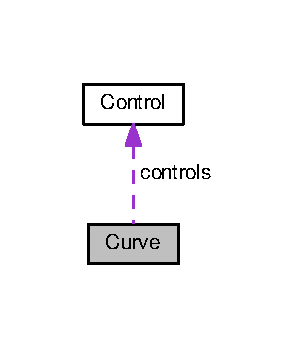
\includegraphics[width=142pt]{struct_curve__coll__graph}
\end{center}
\end{figure}
\subsection*{Data Fields}
\begin{DoxyCompactItemize}
\item 
int \hyperlink{struct_curve_a59a5b03dc125415956c7a70d6ca5f1c9}{control\+\_\+count}
\item 
\hyperlink{struct_control}{Control} \hyperlink{struct_curve_a4ee2ee7a61aec07c8125cf99d3aca658}{controls} \mbox{[}C\+O\+N\+T\+R\+O\+L\+\_\+\+M\+AX\mbox{]}
\item 
double \hyperlink{struct_curve_ae0904aba32ac63f201e7b09c5a369801}{shift\+\_\+x}
\item 
double \hyperlink{struct_curve_acf3ad5e60603cbced782bbebef4e0d06}{shift\+\_\+y}
\end{DoxyCompactItemize}


\subsection{Detailed Description}
Objet contenant une courbe. 

\hyperlink{struct_curve}{Curve} est objet contenant une courbe 

\subsection{Field Documentation}
\index{Curve@{Curve}!control\+\_\+count@{control\+\_\+count}}
\index{control\+\_\+count@{control\+\_\+count}!Curve@{Curve}}
\subsubsection[{\texorpdfstring{control\+\_\+count}{control_count}}]{\setlength{\rightskip}{0pt plus 5cm}int control\+\_\+count}\hypertarget{struct_curve_a59a5b03dc125415956c7a70d6ca5f1c9}{}\label{struct_curve_a59a5b03dc125415956c7a70d6ca5f1c9}
Nombre des points de controls. \index{Curve@{Curve}!controls@{controls}}
\index{controls@{controls}!Curve@{Curve}}
\subsubsection[{\texorpdfstring{controls}{controls}}]{\setlength{\rightskip}{0pt plus 5cm}{\bf Control} controls\mbox{[}C\+O\+N\+T\+R\+O\+L\+\_\+\+M\+AX\mbox{]}}\hypertarget{struct_curve_a4ee2ee7a61aec07c8125cf99d3aca658}{}\label{struct_curve_a4ee2ee7a61aec07c8125cf99d3aca658}
Tableau de point de control. \index{Curve@{Curve}!shift\+\_\+x@{shift\+\_\+x}}
\index{shift\+\_\+x@{shift\+\_\+x}!Curve@{Curve}}
\subsubsection[{\texorpdfstring{shift\+\_\+x}{shift_x}}]{\setlength{\rightskip}{0pt plus 5cm}double shift\+\_\+x}\hypertarget{struct_curve_ae0904aba32ac63f201e7b09c5a369801}{}\label{struct_curve_ae0904aba32ac63f201e7b09c5a369801}
Shift y. \index{Curve@{Curve}!shift\+\_\+y@{shift\+\_\+y}}
\index{shift\+\_\+y@{shift\+\_\+y}!Curve@{Curve}}
\subsubsection[{\texorpdfstring{shift\+\_\+y}{shift_y}}]{\setlength{\rightskip}{0pt plus 5cm}double shift\+\_\+y}\hypertarget{struct_curve_acf3ad5e60603cbced782bbebef4e0d06}{}\label{struct_curve_acf3ad5e60603cbced782bbebef4e0d06}
Shift y. 

The documentation for this struct was generated from the following file\+:\begin{DoxyCompactItemize}
\item 
\hyperlink{curve_8h}{curve.\+h}\end{DoxyCompactItemize}

\hypertarget{struct_curve__infos}{}\section{Curve\+\_\+infos Struct Reference}
\label{struct_curve__infos}\index{Curve\+\_\+infos@{Curve\+\_\+infos}}


Objet contenant une curve\+\_\+list ainsi que la courbe courante et le point de control courant.  




{\ttfamily \#include $<$curve.\+h$>$}



Collaboration diagram for Curve\+\_\+infos\+:
\nopagebreak
\begin{figure}[H]
\begin{center}
\leavevmode
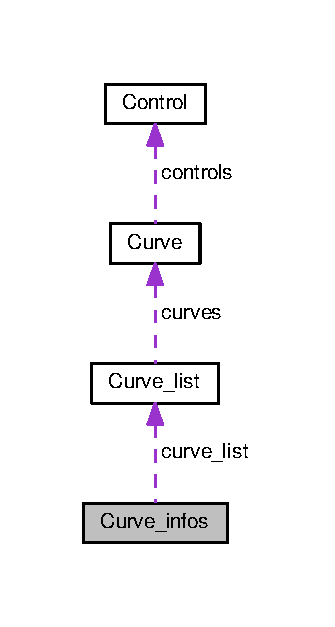
\includegraphics[width=161pt]{struct_curve__infos__coll__graph}
\end{center}
\end{figure}
\subsection*{Data Fields}
\begin{DoxyCompactItemize}
\item 
\hyperlink{struct_curve__list}{Curve\+\_\+list} \hyperlink{struct_curve__infos_ac27e69087504043a258d19abcaa6cc95}{curve\+\_\+list}
\item 
int \hyperlink{struct_curve__infos_a1dfb6df9eb8f617d17265d99305c8464}{current\+\_\+curve}
\item 
int \hyperlink{struct_curve__infos_ac29ff01cfeacc113317497e57f0bd892}{current\+\_\+control}
\end{DoxyCompactItemize}


\subsection{Detailed Description}
Objet contenant une curve\+\_\+list ainsi que la courbe courante et le point de control courant. 

\hyperlink{struct_curve__infos}{Curve\+\_\+infos} est un objet contenant une curve\+\_\+list ainsi que la courbe courante et le point de control courant. 

\subsection{Field Documentation}
\index{Curve\+\_\+infos@{Curve\+\_\+infos}!current\+\_\+control@{current\+\_\+control}}
\index{current\+\_\+control@{current\+\_\+control}!Curve\+\_\+infos@{Curve\+\_\+infos}}
\subsubsection[{\texorpdfstring{current\+\_\+control}{current_control}}]{\setlength{\rightskip}{0pt plus 5cm}int current\+\_\+control}\hypertarget{struct_curve__infos_ac29ff01cfeacc113317497e57f0bd892}{}\label{struct_curve__infos_ac29ff01cfeacc113317497e57f0bd892}
Point de control courant. \index{Curve\+\_\+infos@{Curve\+\_\+infos}!current\+\_\+curve@{current\+\_\+curve}}
\index{current\+\_\+curve@{current\+\_\+curve}!Curve\+\_\+infos@{Curve\+\_\+infos}}
\subsubsection[{\texorpdfstring{current\+\_\+curve}{current_curve}}]{\setlength{\rightskip}{0pt plus 5cm}int current\+\_\+curve}\hypertarget{struct_curve__infos_a1dfb6df9eb8f617d17265d99305c8464}{}\label{struct_curve__infos_a1dfb6df9eb8f617d17265d99305c8464}
Courbe courante. \index{Curve\+\_\+infos@{Curve\+\_\+infos}!curve\+\_\+list@{curve\+\_\+list}}
\index{curve\+\_\+list@{curve\+\_\+list}!Curve\+\_\+infos@{Curve\+\_\+infos}}
\subsubsection[{\texorpdfstring{curve\+\_\+list}{curve_list}}]{\setlength{\rightskip}{0pt plus 5cm}{\bf Curve\+\_\+list} curve\+\_\+list}\hypertarget{struct_curve__infos_ac27e69087504043a258d19abcaa6cc95}{}\label{struct_curve__infos_ac27e69087504043a258d19abcaa6cc95}
Objet curve\+\_\+list. 

The documentation for this struct was generated from the following file\+:\begin{DoxyCompactItemize}
\item 
\hyperlink{curve_8h}{curve.\+h}\end{DoxyCompactItemize}

\hypertarget{struct_curve__list}{}\section{Curve\+\_\+list Struct Reference}
\label{struct_curve__list}\index{Curve\+\_\+list@{Curve\+\_\+list}}


Objet contenant un tableau de curve ainsi que le nombre de ces curves.  




{\ttfamily \#include $<$curve.\+h$>$}



Collaboration diagram for Curve\+\_\+list\+:
\nopagebreak
\begin{figure}[H]
\begin{center}
\leavevmode
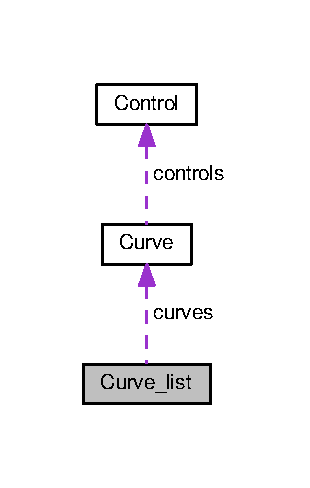
\includegraphics[width=149pt]{struct_curve__list__coll__graph}
\end{center}
\end{figure}
\subsection*{Data Fields}
\begin{DoxyCompactItemize}
\item 
int \hyperlink{struct_curve__list_a97c088ae642b601e713d2001c718864d}{curve\+\_\+count}
\item 
\hyperlink{struct_curve}{Curve} \hyperlink{struct_curve__list_a55c0ff2f9889340ccae2f1b414a2f482}{curves} \mbox{[}C\+U\+R\+V\+E\+\_\+\+M\+AX\mbox{]}
\end{DoxyCompactItemize}


\subsection{Detailed Description}
Objet contenant un tableau de curve ainsi que le nombre de ces curves. 

\hyperlink{struct_curve__list}{Curve\+\_\+list} est objet contenant un tableau de curve ainsi que le nombre de ces curves. 

\subsection{Field Documentation}
\index{Curve\+\_\+list@{Curve\+\_\+list}!curve\+\_\+count@{curve\+\_\+count}}
\index{curve\+\_\+count@{curve\+\_\+count}!Curve\+\_\+list@{Curve\+\_\+list}}
\subsubsection[{\texorpdfstring{curve\+\_\+count}{curve_count}}]{\setlength{\rightskip}{0pt plus 5cm}int curve\+\_\+count}\hypertarget{struct_curve__list_a97c088ae642b601e713d2001c718864d}{}\label{struct_curve__list_a97c088ae642b601e713d2001c718864d}
Nombre de courbe. \index{Curve\+\_\+list@{Curve\+\_\+list}!curves@{curves}}
\index{curves@{curves}!Curve\+\_\+list@{Curve\+\_\+list}}
\subsubsection[{\texorpdfstring{curves}{curves}}]{\setlength{\rightskip}{0pt plus 5cm}{\bf Curve} curves\mbox{[}C\+U\+R\+V\+E\+\_\+\+M\+AX\mbox{]}}\hypertarget{struct_curve__list_a55c0ff2f9889340ccae2f1b414a2f482}{}\label{struct_curve__list_a55c0ff2f9889340ccae2f1b414a2f482}
Tableau des courbes. 

The documentation for this struct was generated from the following file\+:\begin{DoxyCompactItemize}
\item 
\hyperlink{curve_8h}{curve.\+h}\end{DoxyCompactItemize}

\hypertarget{struct_game}{}\section{Game Struct Reference}
\label{struct_game}\index{Game@{Game}}


Objet contenant les informations pour un \hyperlink{struct_game}{Game}.  




{\ttfamily \#include $<$game.\+h$>$}



Collaboration diagram for Game\+:
\nopagebreak
\begin{figure}[H]
\begin{center}
\leavevmode
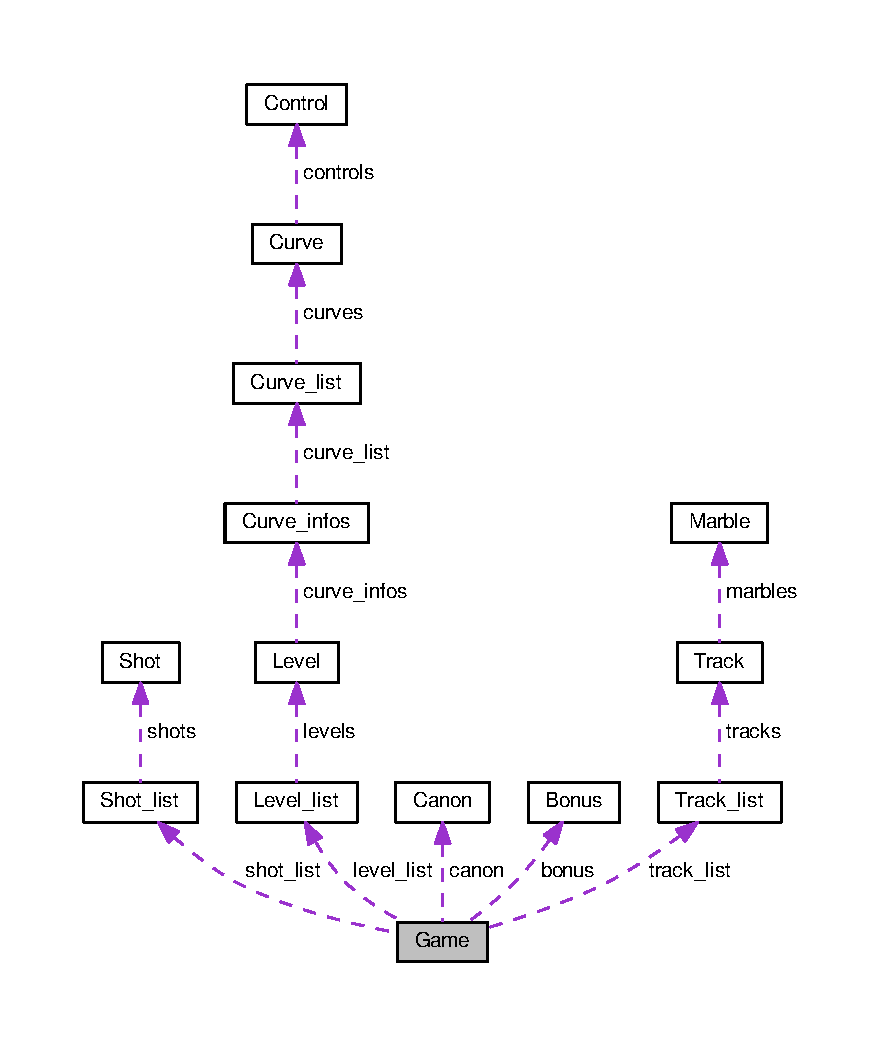
\includegraphics[width=350pt]{struct_game__coll__graph}
\end{center}
\end{figure}
\subsection*{Data Fields}
\begin{DoxyCompactItemize}
\item 
\hyperlink{game_8h_a33e243da48884e73997b5c5fa62864d4}{Game\+\_\+state} \hyperlink{struct_game_abe9c6b7e729dc8fdac044b9a37ec19f3}{state}
\item 
\hyperlink{struct_bonus}{Bonus} \hyperlink{struct_game_ad9bc80a3bd450dcd9f2c68c2e523051d}{bonus}
\item 
int \hyperlink{struct_game_aadd67ce7858be05c138c310167fcf663}{current\+\_\+level}
\item 
int \hyperlink{struct_game_aef160b7437d94056f1dc59646cd5b87d}{score}
\item 
int \hyperlink{struct_game_aa59e6d9166b7c819a741e5738d7edb4a}{score\+\_\+level\+\_\+before}
\item 
int \hyperlink{struct_game_a740c72199e905a6e7b1465e539ce9405}{level\+Sup\+Speed\+Malus}
\item 
\hyperlink{struct_canon}{Canon} \hyperlink{struct_game_a842d6f5ebfe8dd375e5b03e080622d93}{canon}
\item 
\hyperlink{struct_shot__list}{Shot\+\_\+list} \hyperlink{struct_game_ad9d344b557c1fa1dcf5707e3009feb07}{shot\+\_\+list}
\item 
\hyperlink{struct_track__list}{Track\+\_\+list} \hyperlink{struct_game_a3a80b48316d096cc230b63eb95214c36}{track\+\_\+list}
\item 
\hyperlink{struct_level__list}{Level\+\_\+list} \hyperlink{struct_game_a592a02fc63fe476f0b4fabe6240a24b8}{level\+\_\+list}
\end{DoxyCompactItemize}


\subsection{Detailed Description}
Objet contenant les informations pour un \hyperlink{struct_game}{Game}. 

Objet contenant les informations pour un \hyperlink{struct_game}{Game} Game\+\_\+state state; \hyperlink{struct_bonus}{Bonus} bonus; int current\+\_\+level; int score; int score\+\_\+level\+\_\+before; int level\+Sup\+Speed\+Malus; \hyperlink{struct_canon}{Canon} canon; \hyperlink{struct_shot__list}{Shot\+\_\+list} shot\+\_\+list; \hyperlink{struct_track__list}{Track\+\_\+list} track\+\_\+list; \hyperlink{struct_level__list}{Level\+\_\+list} level\+\_\+list; 

\subsection{Field Documentation}
\index{Game@{Game}!bonus@{bonus}}
\index{bonus@{bonus}!Game@{Game}}
\subsubsection[{\texorpdfstring{bonus}{bonus}}]{\setlength{\rightskip}{0pt plus 5cm}{\bf Bonus} bonus}\hypertarget{struct_game_ad9bc80a3bd450dcd9f2c68c2e523051d}{}\label{struct_game_ad9bc80a3bd450dcd9f2c68c2e523051d}
État du jeu. \index{Game@{Game}!canon@{canon}}
\index{canon@{canon}!Game@{Game}}
\subsubsection[{\texorpdfstring{canon}{canon}}]{\setlength{\rightskip}{0pt plus 5cm}{\bf Canon} canon}\hypertarget{struct_game_a842d6f5ebfe8dd375e5b03e080622d93}{}\label{struct_game_a842d6f5ebfe8dd375e5b03e080622d93}
Objet \hyperlink{struct_canon}{Canon}. \index{Game@{Game}!current\+\_\+level@{current\+\_\+level}}
\index{current\+\_\+level@{current\+\_\+level}!Game@{Game}}
\subsubsection[{\texorpdfstring{current\+\_\+level}{current_level}}]{\setlength{\rightskip}{0pt plus 5cm}int current\+\_\+level}\hypertarget{struct_game_aadd67ce7858be05c138c310167fcf663}{}\label{struct_game_aadd67ce7858be05c138c310167fcf663}
\hyperlink{struct_level}{Level} courant. \index{Game@{Game}!level\+\_\+list@{level\+\_\+list}}
\index{level\+\_\+list@{level\+\_\+list}!Game@{Game}}
\subsubsection[{\texorpdfstring{level\+\_\+list}{level_list}}]{\setlength{\rightskip}{0pt plus 5cm}{\bf Level\+\_\+list} level\+\_\+list}\hypertarget{struct_game_a592a02fc63fe476f0b4fabe6240a24b8}{}\label{struct_game_a592a02fc63fe476f0b4fabe6240a24b8}
Liste des levels. \index{Game@{Game}!level\+Sup\+Speed\+Malus@{level\+Sup\+Speed\+Malus}}
\index{level\+Sup\+Speed\+Malus@{level\+Sup\+Speed\+Malus}!Game@{Game}}
\subsubsection[{\texorpdfstring{level\+Sup\+Speed\+Malus}{levelSupSpeedMalus}}]{\setlength{\rightskip}{0pt plus 5cm}int level\+Sup\+Speed\+Malus}\hypertarget{struct_game_a740c72199e905a6e7b1465e539ce9405}{}\label{struct_game_a740c72199e905a6e7b1465e539ce9405}
Malus vitesse après retour au level 0 après avoir gagné les de 0 à 10 levels. \index{Game@{Game}!score@{score}}
\index{score@{score}!Game@{Game}}
\subsubsection[{\texorpdfstring{score}{score}}]{\setlength{\rightskip}{0pt plus 5cm}int score}\hypertarget{struct_game_aef160b7437d94056f1dc59646cd5b87d}{}\label{struct_game_aef160b7437d94056f1dc59646cd5b87d}
Score. \index{Game@{Game}!score\+\_\+level\+\_\+before@{score\+\_\+level\+\_\+before}}
\index{score\+\_\+level\+\_\+before@{score\+\_\+level\+\_\+before}!Game@{Game}}
\subsubsection[{\texorpdfstring{score\+\_\+level\+\_\+before}{score_level_before}}]{\setlength{\rightskip}{0pt plus 5cm}int score\+\_\+level\+\_\+before}\hypertarget{struct_game_aa59e6d9166b7c819a741e5738d7edb4a}{}\label{struct_game_aa59e6d9166b7c819a741e5738d7edb4a}
État du jeu. \index{Game@{Game}!shot\+\_\+list@{shot\+\_\+list}}
\index{shot\+\_\+list@{shot\+\_\+list}!Game@{Game}}
\subsubsection[{\texorpdfstring{shot\+\_\+list}{shot_list}}]{\setlength{\rightskip}{0pt plus 5cm}{\bf Shot\+\_\+list} shot\+\_\+list}\hypertarget{struct_game_ad9d344b557c1fa1dcf5707e3009feb07}{}\label{struct_game_ad9d344b557c1fa1dcf5707e3009feb07}
Liste des shots tirés. \index{Game@{Game}!state@{state}}
\index{state@{state}!Game@{Game}}
\subsubsection[{\texorpdfstring{state}{state}}]{\setlength{\rightskip}{0pt plus 5cm}{\bf Game\+\_\+state} state}\hypertarget{struct_game_abe9c6b7e729dc8fdac044b9a37ec19f3}{}\label{struct_game_abe9c6b7e729dc8fdac044b9a37ec19f3}
État du jeu. \index{Game@{Game}!track\+\_\+list@{track\+\_\+list}}
\index{track\+\_\+list@{track\+\_\+list}!Game@{Game}}
\subsubsection[{\texorpdfstring{track\+\_\+list}{track_list}}]{\setlength{\rightskip}{0pt plus 5cm}{\bf Track\+\_\+list} track\+\_\+list}\hypertarget{struct_game_a3a80b48316d096cc230b63eb95214c36}{}\label{struct_game_a3a80b48316d096cc230b63eb95214c36}
Liste des tracks. 

The documentation for this struct was generated from the following file\+:\begin{DoxyCompactItemize}
\item 
\hyperlink{game_8h}{game.\+h}\end{DoxyCompactItemize}

\hypertarget{struct_level}{}\section{Level Struct Reference}
\label{struct_level}\index{Level@{Level}}


Objet contenant les informations pour un \hyperlink{struct_level}{Level}.  




{\ttfamily \#include $<$game.\+h$>$}



Collaboration diagram for Level\+:
\nopagebreak
\begin{figure}[H]
\begin{center}
\leavevmode
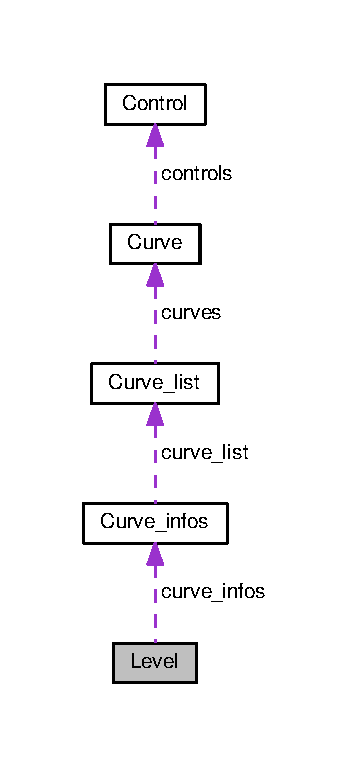
\includegraphics[width=169pt]{struct_level__coll__graph}
\end{center}
\end{figure}
\subsection*{Data Fields}
\begin{DoxyCompactItemize}
\item 
\hyperlink{struct_curve__infos}{Curve\+\_\+infos} \hyperlink{struct_level_a917c9ea829deeac9d6a1c2309f76595b}{curve\+\_\+infos}
\item 
double \hyperlink{struct_level_a8d69c9e5161432eba15b8c66a3d822dc}{canon\+\_\+x}
\item 
double \hyperlink{struct_level_ae539e37b2953880bd182e39068838d1a}{canon\+\_\+y}
\item 
int \hyperlink{struct_level_a49a2ee16a8bedba06cdd451170c2e5ad}{marbles\+\_\+intro}
\item 
int \hyperlink{struct_level_a96e2ff7aa7e440993d021792df0fcfd3}{marbles\+\_\+total}
\end{DoxyCompactItemize}


\subsection{Detailed Description}
Objet contenant les informations pour un \hyperlink{struct_level}{Level}. 

Objet contenant les informations pour un \hyperlink{struct_level}{Level}, non utilisé pour le moment car le nombre de bille d\textquotesingle{}intro et total est calculé avec une fonction quant à la position du canon elle est fixe \hyperlink{struct_curve__infos}{Curve\+\_\+infos} curve\+\_\+infos; double canon\+\_\+x, canon\+\_\+y; int marbles\+\_\+intro, marbles\+\_\+total; 

\subsection{Field Documentation}
\index{Level@{Level}!canon\+\_\+x@{canon\+\_\+x}}
\index{canon\+\_\+x@{canon\+\_\+x}!Level@{Level}}
\subsubsection[{\texorpdfstring{canon\+\_\+x}{canon_x}}]{\setlength{\rightskip}{0pt plus 5cm}double canon\+\_\+x}\hypertarget{struct_level_a8d69c9e5161432eba15b8c66a3d822dc}{}\label{struct_level_a8d69c9e5161432eba15b8c66a3d822dc}
Position x du canon. \index{Level@{Level}!canon\+\_\+y@{canon\+\_\+y}}
\index{canon\+\_\+y@{canon\+\_\+y}!Level@{Level}}
\subsubsection[{\texorpdfstring{canon\+\_\+y}{canon_y}}]{\setlength{\rightskip}{0pt plus 5cm}double canon\+\_\+y}\hypertarget{struct_level_ae539e37b2953880bd182e39068838d1a}{}\label{struct_level_ae539e37b2953880bd182e39068838d1a}
Position y du canon. \index{Level@{Level}!curve\+\_\+infos@{curve\+\_\+infos}}
\index{curve\+\_\+infos@{curve\+\_\+infos}!Level@{Level}}
\subsubsection[{\texorpdfstring{curve\+\_\+infos}{curve_infos}}]{\setlength{\rightskip}{0pt plus 5cm}{\bf Curve\+\_\+infos} curve\+\_\+infos}\hypertarget{struct_level_a917c9ea829deeac9d6a1c2309f76595b}{}\label{struct_level_a917c9ea829deeac9d6a1c2309f76595b}
La track du level sous forme de curve. \index{Level@{Level}!marbles\+\_\+intro@{marbles\+\_\+intro}}
\index{marbles\+\_\+intro@{marbles\+\_\+intro}!Level@{Level}}
\subsubsection[{\texorpdfstring{marbles\+\_\+intro}{marbles_intro}}]{\setlength{\rightskip}{0pt plus 5cm}int marbles\+\_\+intro}\hypertarget{struct_level_a49a2ee16a8bedba06cdd451170c2e5ad}{}\label{struct_level_a49a2ee16a8bedba06cdd451170c2e5ad}
Nombre de marble à l\textquotesingle{}intro. \index{Level@{Level}!marbles\+\_\+total@{marbles\+\_\+total}}
\index{marbles\+\_\+total@{marbles\+\_\+total}!Level@{Level}}
\subsubsection[{\texorpdfstring{marbles\+\_\+total}{marbles_total}}]{\setlength{\rightskip}{0pt plus 5cm}int marbles\+\_\+total}\hypertarget{struct_level_a96e2ff7aa7e440993d021792df0fcfd3}{}\label{struct_level_a96e2ff7aa7e440993d021792df0fcfd3}
Nombre de marble total. 

The documentation for this struct was generated from the following file\+:\begin{DoxyCompactItemize}
\item 
\hyperlink{game_8h}{game.\+h}\end{DoxyCompactItemize}

\hypertarget{struct_level__list}{}\section{Level\+\_\+list Struct Reference}
\label{struct_level__list}\index{Level\+\_\+list@{Level\+\_\+list}}


Objet contenant les informations pour un \hyperlink{struct_level__list}{Level\+\_\+list}.  




{\ttfamily \#include $<$game.\+h$>$}



Collaboration diagram for Level\+\_\+list\+:
\nopagebreak
\begin{figure}[H]
\begin{center}
\leavevmode
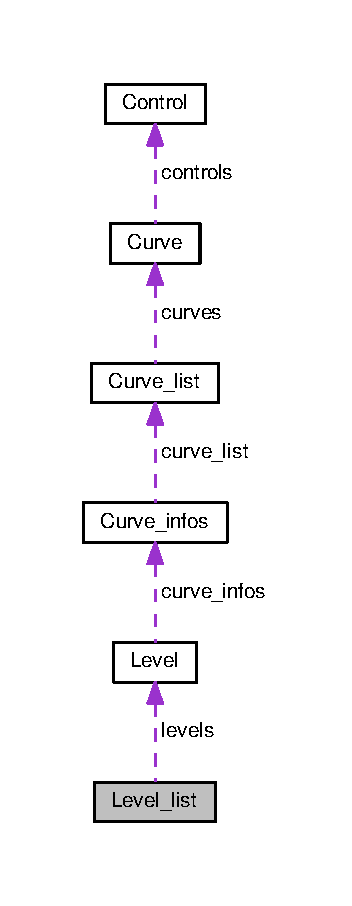
\includegraphics[width=169pt]{struct_level__list__coll__graph}
\end{center}
\end{figure}
\subsection*{Data Fields}
\begin{DoxyCompactItemize}
\item 
int \hyperlink{struct_level__list_a15a1d581c38f5a80cf12ac022ad6c600}{level\+\_\+count}
\item 
\hyperlink{struct_level}{Level} \hyperlink{struct_level__list_a3dc8b993b65462f76626717e082e4e72}{levels} \mbox{[}L\+E\+V\+E\+L\+\_\+\+M\+AX+1\mbox{]}
\end{DoxyCompactItemize}


\subsection{Detailed Description}
Objet contenant les informations pour un \hyperlink{struct_level__list}{Level\+\_\+list}. 

Objet contenant les informations pour un \hyperlink{struct_level__list}{Level\+\_\+list}, non utilisé pour le moment car le level est chargé au changement et non au début du jeu int level\+\_\+count; \hyperlink{struct_level}{Level} levels\mbox{[}L\+E\+V\+E\+L\+\_\+\+M\+AX\mbox{]}; 

\subsection{Field Documentation}
\index{Level\+\_\+list@{Level\+\_\+list}!level\+\_\+count@{level\+\_\+count}}
\index{level\+\_\+count@{level\+\_\+count}!Level\+\_\+list@{Level\+\_\+list}}
\subsubsection[{\texorpdfstring{level\+\_\+count}{level_count}}]{\setlength{\rightskip}{0pt plus 5cm}int level\+\_\+count}\hypertarget{struct_level__list_a15a1d581c38f5a80cf12ac022ad6c600}{}\label{struct_level__list_a15a1d581c38f5a80cf12ac022ad6c600}
Nombre de level max actuellement. \index{Level\+\_\+list@{Level\+\_\+list}!levels@{levels}}
\index{levels@{levels}!Level\+\_\+list@{Level\+\_\+list}}
\subsubsection[{\texorpdfstring{levels}{levels}}]{\setlength{\rightskip}{0pt plus 5cm}{\bf Level} levels\mbox{[}L\+E\+V\+E\+L\+\_\+\+M\+AX+1\mbox{]}}\hypertarget{struct_level__list_a3dc8b993b65462f76626717e082e4e72}{}\label{struct_level__list_a3dc8b993b65462f76626717e082e4e72}
Liste des levels. 

The documentation for this struct was generated from the following file\+:\begin{DoxyCompactItemize}
\item 
\hyperlink{game_8h}{game.\+h}\end{DoxyCompactItemize}

\hypertarget{struct_marble}{}\section{Marble Struct Reference}
\label{struct_marble}\index{Marble@{Marble}}


Objet contenant les informations pour un \hyperlink{struct_marble}{Marble}.  




{\ttfamily \#include $<$game.\+h$>$}

\subsection*{Data Fields}
\begin{DoxyCompactItemize}
\item 
double \hyperlink{struct_marble_af88b946fb90d5f08b5fb740c70e98c10}{x}
\item 
double \hyperlink{struct_marble_ab927965981178aa1fba979a37168db2a}{y}
\item 
double \hyperlink{struct_marble_a87accd1af8e0aff4b818d891374f7cec}{t}
\item 
int \hyperlink{struct_marble_a0fd02fb9277ffcb35a75066ffe95e8c7}{color}
\item 
int {\bfseries is\+\_\+combo\+\_\+end}\hypertarget{struct_marble_a6ac94ef9db7b26b611b521b74e906407}{}\label{struct_marble_a6ac94ef9db7b26b611b521b74e906407}

\item 
int {\bfseries step\+\_\+explode}\hypertarget{struct_marble_adeeb3b358209448342b64c549b46759e}{}\label{struct_marble_adeeb3b358209448342b64c549b46759e}

\item 
int \hyperlink{struct_marble_a21a6e1305c3f396d42ee151e8751b469}{bonus}
\end{DoxyCompactItemize}


\subsection{Detailed Description}
Objet contenant les informations pour un \hyperlink{struct_marble}{Marble}. 

Objet contenant les informations pour un \hyperlink{struct_marble}{Marble} double x, y; // coordonnées centre double t; // paramètre dans l\textquotesingle{}échantillonnage int color; int is\+\_\+combo\+\_\+end; // ou encore, facteur vitesse et direction ? int step\+\_\+explode; int bonus; 

\subsection{Field Documentation}
\index{Marble@{Marble}!bonus@{bonus}}
\index{bonus@{bonus}!Marble@{Marble}}
\subsubsection[{\texorpdfstring{bonus}{bonus}}]{\setlength{\rightskip}{0pt plus 5cm}int bonus}\hypertarget{struct_marble_a21a6e1305c3f396d42ee151e8751b469}{}\label{struct_marble_a21a6e1305c3f396d42ee151e8751b469}
\hyperlink{struct_bonus}{Bonus} de la bille. \index{Marble@{Marble}!color@{color}}
\index{color@{color}!Marble@{Marble}}
\subsubsection[{\texorpdfstring{color}{color}}]{\setlength{\rightskip}{0pt plus 5cm}int color}\hypertarget{struct_marble_a0fd02fb9277ffcb35a75066ffe95e8c7}{}\label{struct_marble_a0fd02fb9277ffcb35a75066ffe95e8c7}
Couleur de la bille. \index{Marble@{Marble}!t@{t}}
\index{t@{t}!Marble@{Marble}}
\subsubsection[{\texorpdfstring{t}{t}}]{\setlength{\rightskip}{0pt plus 5cm}double t}\hypertarget{struct_marble_a87accd1af8e0aff4b818d891374f7cec}{}\label{struct_marble_a87accd1af8e0aff4b818d891374f7cec}
paramètre dans l\textquotesingle{}échantillonnage. \index{Marble@{Marble}!x@{x}}
\index{x@{x}!Marble@{Marble}}
\subsubsection[{\texorpdfstring{x}{x}}]{\setlength{\rightskip}{0pt plus 5cm}double x}\hypertarget{struct_marble_af88b946fb90d5f08b5fb740c70e98c10}{}\label{struct_marble_af88b946fb90d5f08b5fb740c70e98c10}
coordonnées centre x. \index{Marble@{Marble}!y@{y}}
\index{y@{y}!Marble@{Marble}}
\subsubsection[{\texorpdfstring{y}{y}}]{\setlength{\rightskip}{0pt plus 5cm}double y}\hypertarget{struct_marble_ab927965981178aa1fba979a37168db2a}{}\label{struct_marble_ab927965981178aa1fba979a37168db2a}
coordonnées centre y. 

The documentation for this struct was generated from the following file\+:\begin{DoxyCompactItemize}
\item 
\hyperlink{game_8h}{game.\+h}\end{DoxyCompactItemize}

\hypertarget{struct_mydata}{}\section{Mydata Struct Reference}
\label{struct_mydata}\index{Mydata@{Mydata}}


Objet contenant les informations pour un \hyperlink{struct_mydata}{Mydata}.  




{\ttfamily \#include $<$mydata.\+h$>$}



Collaboration diagram for Mydata\+:
\nopagebreak
\begin{figure}[H]
\begin{center}
\leavevmode
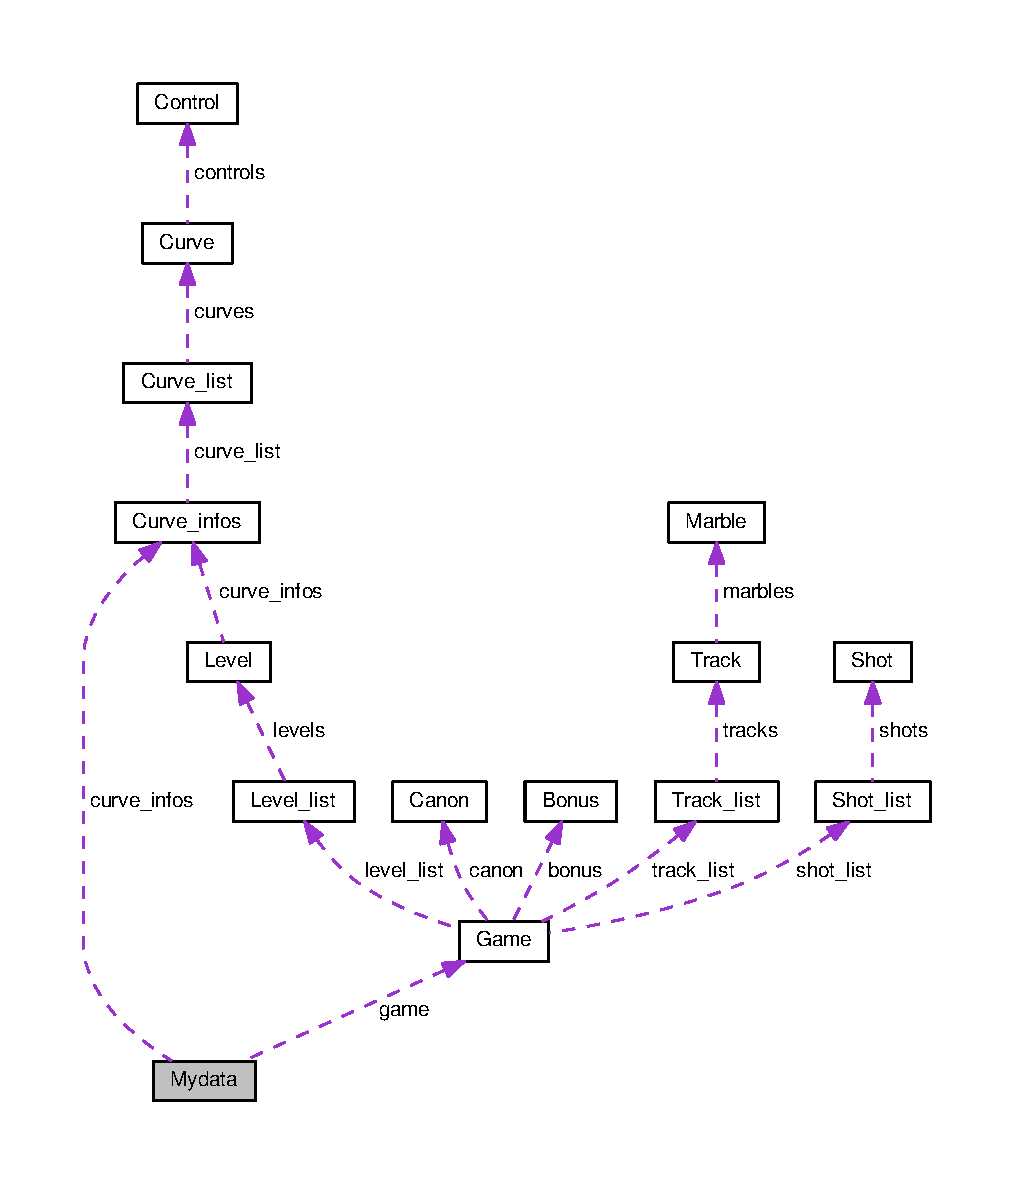
\includegraphics[width=350pt]{struct_mydata__coll__graph}
\end{center}
\end{figure}
\subsection*{Data Fields}
\begin{DoxyCompactItemize}
\item 
Gtk\+Widget $\ast$ \hyperlink{struct_mydata_a3d346c08cf2d67c388caabffb412b293}{window}
\item 
Gtk\+Widget $\ast$ \hyperlink{struct_mydata_ab8c991d830297ad3502ab72c109e6fe7}{status}
\item 
Gtk\+Widget $\ast$ \hyperlink{struct_mydata_a4135ce280f2ff654540c78e33ce96228}{vbox}
\item 
Gtk\+Widget $\ast$ \hyperlink{struct_mydata_a790d57ae229197048b24b1b0fdacc701}{area}
\item 
Gtk\+Widget $\ast$ \hyperlink{struct_mydata_abf79962e7a3ee4a5c5ef80b4058ce491}{scroll}
\item 
Gtk\+Widget $\ast$ \hyperlink{struct_mydata_ad2f34f578fffe42cf2686e61f2dd85bf}{menu\+\_\+bar}
\item 
Gtk\+Widget $\ast$ \hyperlink{struct_mydata_aa96506ac11851965d0f25b0c9eb53885}{frame}
\item 
Gtk\+Widget $\ast$ \hyperlink{struct_mydata_ad9fd4a843722e81542171abbef74f968}{player\+Stats\+Frame}
\item 
Gtk\+Widget $\ast$ \hyperlink{struct_mydata_a27bc5fb5d105194b992c82a95d408222}{level\+Label}
\item 
Gtk\+Widget $\ast$ \hyperlink{struct_mydata_ae067b2d6b08b38aa73b035c82d9e14b0}{score\+Label}
\item 
Gtk\+Widget $\ast$ \hyperlink{struct_mydata_a8f7df3b38dd2aa1d9d7e1bf4276c1d53}{player\+Progress}
\item 
Gtk\+Widget $\ast$ \hyperlink{struct_mydata_ab7e5d6396dfecd2bc73d0114bf4de49c}{bonus\+Label}
\item 
Gtk\+Widget $\ast$ \hyperlink{struct_mydata_a1eed6d0ed7438018e0d938fce66d265d}{hbox}
\item 
Gtk\+Widget $\ast$ {\bfseries add\+\_\+curve}\hypertarget{struct_mydata_afa41b812a39706ff35d77f730089dbf1}{}\label{struct_mydata_afa41b812a39706ff35d77f730089dbf1}

\item 
Gtk\+Widget $\ast$ {\bfseries move\+\_\+curve}\hypertarget{struct_mydata_a62f7075fccfcca150953f1b266bc86d6}{}\label{struct_mydata_a62f7075fccfcca150953f1b266bc86d6}

\item 
Gtk\+Widget $\ast$ {\bfseries remove\+\_\+curve}\hypertarget{struct_mydata_a475e6d0f2736d7bd94a895fe0423569a}{}\label{struct_mydata_a475e6d0f2736d7bd94a895fe0423569a}

\item 
Gtk\+Widget $\ast$ {\bfseries add\+\_\+control}\hypertarget{struct_mydata_af8a44420fb1b82f2d37ed6609d70b5dd}{}\label{struct_mydata_af8a44420fb1b82f2d37ed6609d70b5dd}

\item 
Gtk\+Widget $\ast$ {\bfseries move\+\_\+control}\hypertarget{struct_mydata_a80d44897e2754069918981b06206496c}{}\label{struct_mydata_a80d44897e2754069918981b06206496c}

\item 
Gtk\+Widget $\ast$ {\bfseries remove\+\_\+control}\hypertarget{struct_mydata_a7e9b035533ac6db7c3318a82707e02dc}{}\label{struct_mydata_a7e9b035533ac6db7c3318a82707e02dc}

\item 
Gtk\+Widget $\ast$ {\bfseries vertical}\hypertarget{struct_mydata_a0d1463efb2dd75d7a39d3f6b5b60029f}{}\label{struct_mydata_a0d1463efb2dd75d7a39d3f6b5b60029f}

\item 
Gtk\+Widget $\ast$ \hyperlink{struct_mydata_afeceefa9528b56c22e00612af53c8272}{edit\+\_\+radios} \mbox{[}E\+D\+I\+T\+\_\+\+L\+A\+ST\mbox{]}
\item 
Gtk\+Widget $\ast$ \hyperlink{struct_mydata_af0129a7558616569b70f65f56fd2aed0}{bsp\+\_\+radios} \mbox{[}B\+S\+P\+\_\+\+L\+A\+ST\mbox{]}
\item 
Gdk\+Pixbuf $\ast$ \hyperlink{struct_mydata_a44cf4bc3a3a7376477b86bae6580de08}{pixbuf}
\item 
double \hyperlink{struct_mydata_a49a0f74fc7cb65d2a8ba39006d9e5056}{click\+\_\+x}
\item 
double \hyperlink{struct_mydata_ad50bebb00d8beaa505e312f9597a41a5}{click\+\_\+y}
\item 
double \hyperlink{struct_mydata_abb66b33c1e9a8a118c99e73d77ed512c}{last\+\_\+x}
\item 
double \hyperlink{struct_mydata_a58471f12beade2e129004d30fe0892c1}{last\+\_\+y}
\item 
int \hyperlink{struct_mydata_a3f05049836bf74dcfbc800d417bedec3}{win\+\_\+width}
\item 
int \hyperlink{struct_mydata_a043cefe0d8f27979f9813b61305f1407}{win\+\_\+height}
\item 
int \hyperlink{struct_mydata_ac21cca965335aa0a329dc6029f743542}{show\+\_\+edit}
\item 
int \hyperlink{struct_mydata_a7e53a3b3c1cac6e3afebd783728d232c}{edit\+\_\+mode}
\item 
int \hyperlink{struct_mydata_a4cbcc68b0a3ae7651f3363348f4d7456}{click\+\_\+n}
\item 
int \hyperlink{struct_mydata_a2a4a5364f7ffa17761866a77f6a54556}{bsp\+\_\+mode}
\item 
int \hyperlink{struct_mydata_ad43c3812e6d13e0518d9f8b8f463ffcf}{count}
\item 
unsigned int \hyperlink{struct_mydata_a7154179fe070a40c828f7c03f454d4d6}{magic}
\item 
char $\ast$ \hyperlink{struct_mydata_aecf8e6b88573cc04da63f47bfc13a246}{current\+\_\+folder}
\item 
char $\ast$ \hyperlink{struct_mydata_af06d911bb9e05f491ef3da520d03796c}{title}
\item 
\hyperlink{struct_curve__infos}{Curve\+\_\+infos} \hyperlink{struct_mydata_a917c9ea829deeac9d6a1c2309f76595b}{curve\+\_\+infos}
\item 
\hyperlink{struct_game}{Game} \hyperlink{struct_mydata_ac6a5ed6191fcf3a5bf0445921feb4f48}{game}
\end{DoxyCompactItemize}


\subsection{Detailed Description}
Objet contenant les informations pour un \hyperlink{struct_mydata}{Mydata}. 

Objet contenant les informations pour un \hyperlink{struct_mydata}{Mydata} Gtk\+Widget $\ast$window; Gtk\+Widget $\ast$status; Gtk\+Widget $\ast$vbox; Gtk\+Widget $\ast$area; Gtk\+Widget $\ast$scroll; Gtk\+Widget $\ast$menu\+\_\+bar; Gtk\+Widget $\ast$frame; Gtk\+Widget $\ast$player\+Stats\+Frame; Gtk\+Widget $\ast$level\+Label; Gtk\+Widget $\ast$score\+Label; Gtk\+Widget $\ast$player\+Progress; Gtk\+Widget $\ast$bonus\+Label; Gtk\+Widget $\ast$hbox; Gtk\+Widget $\ast$ add\+\_\+curve; Gtk\+Widget $\ast$ move\+\_\+curve; Gtk\+Widget $\ast$ remove\+\_\+curve; Gtk\+Widget $\ast$ add\+\_\+control; Gtk\+Widget $\ast$ move\+\_\+control; Gtk\+Widget $\ast$ remove\+\_\+control; Gtk\+Widget $\ast$vertical; Gtk\+Widget $\ast$edit\+\_\+radios\mbox{[}E\+D\+I\+T\+\_\+\+L\+A\+ST\mbox{]}; Gtk\+Widget $\ast$bsp\+\_\+radios\mbox{[}B\+S\+P\+\_\+\+L\+A\+ST\mbox{]}; Gdk\+Pixbuf $\ast$pixbuf; double click\+\_\+x; double click\+\_\+y; double last\+\_\+x; double last\+\_\+y; int win\+\_\+width; int win\+\_\+height; int show\+\_\+edit; int edit\+\_\+mode; int click\+\_\+n; int bsp\+\_\+mode; int count; unsigned int magic; char $\ast$ current\+\_\+folder; char $\ast$title; \hyperlink{struct_curve__infos}{Curve\+\_\+infos} curve\+\_\+infos; \hyperlink{struct_game}{Game} game; 

\subsection{Field Documentation}
\index{Mydata@{Mydata}!area@{area}}
\index{area@{area}!Mydata@{Mydata}}
\subsubsection[{\texorpdfstring{area}{area}}]{\setlength{\rightskip}{0pt plus 5cm}Gtk\+Widget$\ast$ area}\hypertarget{struct_mydata_a790d57ae229197048b24b1b0fdacc701}{}\label{struct_mydata_a790d57ae229197048b24b1b0fdacc701}
Area pour dessiner. \index{Mydata@{Mydata}!bonus\+Label@{bonus\+Label}}
\index{bonus\+Label@{bonus\+Label}!Mydata@{Mydata}}
\subsubsection[{\texorpdfstring{bonus\+Label}{bonusLabel}}]{\setlength{\rightskip}{0pt plus 5cm}Gtk\+Widget$\ast$ bonus\+Label}\hypertarget{struct_mydata_ab7e5d6396dfecd2bc73d0114bf4de49c}{}\label{struct_mydata_ab7e5d6396dfecd2bc73d0114bf4de49c}
\hyperlink{struct_bonus}{Bonus} label. \index{Mydata@{Mydata}!bsp\+\_\+mode@{bsp\+\_\+mode}}
\index{bsp\+\_\+mode@{bsp\+\_\+mode}!Mydata@{Mydata}}
\subsubsection[{\texorpdfstring{bsp\+\_\+mode}{bsp_mode}}]{\setlength{\rightskip}{0pt plus 5cm}int bsp\+\_\+mode}\hypertarget{struct_mydata_a2a4a5364f7ffa17761866a77f6a54556}{}\label{struct_mydata_a2a4a5364f7ffa17761866a77f6a54556}
Bsp mode. \index{Mydata@{Mydata}!bsp\+\_\+radios@{bsp\+\_\+radios}}
\index{bsp\+\_\+radios@{bsp\+\_\+radios}!Mydata@{Mydata}}
\subsubsection[{\texorpdfstring{bsp\+\_\+radios}{bsp_radios}}]{\setlength{\rightskip}{0pt plus 5cm}Gtk\+Widget$\ast$ bsp\+\_\+radios\mbox{[}B\+S\+P\+\_\+\+L\+A\+ST\mbox{]}}\hypertarget{struct_mydata_af0129a7558616569b70f65f56fd2aed0}{}\label{struct_mydata_af0129a7558616569b70f65f56fd2aed0}
Tableau bouton radios pour bsp. \index{Mydata@{Mydata}!click\+\_\+n@{click\+\_\+n}}
\index{click\+\_\+n@{click\+\_\+n}!Mydata@{Mydata}}
\subsubsection[{\texorpdfstring{click\+\_\+n}{click_n}}]{\setlength{\rightskip}{0pt plus 5cm}int click\+\_\+n}\hypertarget{struct_mydata_a4cbcc68b0a3ae7651f3363348f4d7456}{}\label{struct_mydata_a4cbcc68b0a3ae7651f3363348f4d7456}
Nombre de click. \index{Mydata@{Mydata}!click\+\_\+x@{click\+\_\+x}}
\index{click\+\_\+x@{click\+\_\+x}!Mydata@{Mydata}}
\subsubsection[{\texorpdfstring{click\+\_\+x}{click_x}}]{\setlength{\rightskip}{0pt plus 5cm}double click\+\_\+x}\hypertarget{struct_mydata_a49a0f74fc7cb65d2a8ba39006d9e5056}{}\label{struct_mydata_a49a0f74fc7cb65d2a8ba39006d9e5056}
coordonnées click x. \index{Mydata@{Mydata}!click\+\_\+y@{click\+\_\+y}}
\index{click\+\_\+y@{click\+\_\+y}!Mydata@{Mydata}}
\subsubsection[{\texorpdfstring{click\+\_\+y}{click_y}}]{\setlength{\rightskip}{0pt plus 5cm}double click\+\_\+y}\hypertarget{struct_mydata_ad50bebb00d8beaa505e312f9597a41a5}{}\label{struct_mydata_ad50bebb00d8beaa505e312f9597a41a5}
coordonnées click y. \index{Mydata@{Mydata}!count@{count}}
\index{count@{count}!Mydata@{Mydata}}
\subsubsection[{\texorpdfstring{count}{count}}]{\setlength{\rightskip}{0pt plus 5cm}int count}\hypertarget{struct_mydata_ad43c3812e6d13e0518d9f8b8f463ffcf}{}\label{struct_mydata_ad43c3812e6d13e0518d9f8b8f463ffcf}
Compteur de passage dans timeout. \index{Mydata@{Mydata}!current\+\_\+folder@{current\+\_\+folder}}
\index{current\+\_\+folder@{current\+\_\+folder}!Mydata@{Mydata}}
\subsubsection[{\texorpdfstring{current\+\_\+folder}{current_folder}}]{\setlength{\rightskip}{0pt plus 5cm}char$\ast$ current\+\_\+folder}\hypertarget{struct_mydata_aecf8e6b88573cc04da63f47bfc13a246}{}\label{struct_mydata_aecf8e6b88573cc04da63f47bfc13a246}
Dossier courant. \index{Mydata@{Mydata}!curve\+\_\+infos@{curve\+\_\+infos}}
\index{curve\+\_\+infos@{curve\+\_\+infos}!Mydata@{Mydata}}
\subsubsection[{\texorpdfstring{curve\+\_\+infos}{curve_infos}}]{\setlength{\rightskip}{0pt plus 5cm}{\bf Curve\+\_\+infos} curve\+\_\+infos}\hypertarget{struct_mydata_a917c9ea829deeac9d6a1c2309f76595b}{}\label{struct_mydata_a917c9ea829deeac9d6a1c2309f76595b}
\hyperlink{struct_curve}{Curve} infos contenant les infos des courbes créé dans l\textquotesingle{}edition. \index{Mydata@{Mydata}!edit\+\_\+mode@{edit\+\_\+mode}}
\index{edit\+\_\+mode@{edit\+\_\+mode}!Mydata@{Mydata}}
\subsubsection[{\texorpdfstring{edit\+\_\+mode}{edit_mode}}]{\setlength{\rightskip}{0pt plus 5cm}int edit\+\_\+mode}\hypertarget{struct_mydata_a7e53a3b3c1cac6e3afebd783728d232c}{}\label{struct_mydata_a7e53a3b3c1cac6e3afebd783728d232c}
Edit mode. \index{Mydata@{Mydata}!edit\+\_\+radios@{edit\+\_\+radios}}
\index{edit\+\_\+radios@{edit\+\_\+radios}!Mydata@{Mydata}}
\subsubsection[{\texorpdfstring{edit\+\_\+radios}{edit_radios}}]{\setlength{\rightskip}{0pt plus 5cm}Gtk\+Widget$\ast$ edit\+\_\+radios\mbox{[}E\+D\+I\+T\+\_\+\+L\+A\+ST\mbox{]}}\hypertarget{struct_mydata_afeceefa9528b56c22e00612af53c8272}{}\label{struct_mydata_afeceefa9528b56c22e00612af53c8272}
Tableau bouton radios pour l\textquotesingle{}edition. \index{Mydata@{Mydata}!frame@{frame}}
\index{frame@{frame}!Mydata@{Mydata}}
\subsubsection[{\texorpdfstring{frame}{frame}}]{\setlength{\rightskip}{0pt plus 5cm}Gtk\+Widget$\ast$ frame}\hypertarget{struct_mydata_aa96506ac11851965d0f25b0c9eb53885}{}\label{struct_mydata_aa96506ac11851965d0f25b0c9eb53885}
Edit frame. \index{Mydata@{Mydata}!game@{game}}
\index{game@{game}!Mydata@{Mydata}}
\subsubsection[{\texorpdfstring{game}{game}}]{\setlength{\rightskip}{0pt plus 5cm}{\bf Game} game}\hypertarget{struct_mydata_ac6a5ed6191fcf3a5bf0445921feb4f48}{}\label{struct_mydata_ac6a5ed6191fcf3a5bf0445921feb4f48}
Objet \hyperlink{struct_game}{Game}. \index{Mydata@{Mydata}!hbox@{hbox}}
\index{hbox@{hbox}!Mydata@{Mydata}}
\subsubsection[{\texorpdfstring{hbox}{hbox}}]{\setlength{\rightskip}{0pt plus 5cm}Gtk\+Widget$\ast$ hbox}\hypertarget{struct_mydata_a1eed6d0ed7438018e0d938fce66d265d}{}\label{struct_mydata_a1eed6d0ed7438018e0d938fce66d265d}
Horizontal box. \index{Mydata@{Mydata}!last\+\_\+x@{last\+\_\+x}}
\index{last\+\_\+x@{last\+\_\+x}!Mydata@{Mydata}}
\subsubsection[{\texorpdfstring{last\+\_\+x}{last_x}}]{\setlength{\rightskip}{0pt plus 5cm}double last\+\_\+x}\hypertarget{struct_mydata_abb66b33c1e9a8a118c99e73d77ed512c}{}\label{struct_mydata_abb66b33c1e9a8a118c99e73d77ed512c}
coordonnées click x precedent. \index{Mydata@{Mydata}!last\+\_\+y@{last\+\_\+y}}
\index{last\+\_\+y@{last\+\_\+y}!Mydata@{Mydata}}
\subsubsection[{\texorpdfstring{last\+\_\+y}{last_y}}]{\setlength{\rightskip}{0pt plus 5cm}double last\+\_\+y}\hypertarget{struct_mydata_a58471f12beade2e129004d30fe0892c1}{}\label{struct_mydata_a58471f12beade2e129004d30fe0892c1}
coordonnées click y precedent. \index{Mydata@{Mydata}!level\+Label@{level\+Label}}
\index{level\+Label@{level\+Label}!Mydata@{Mydata}}
\subsubsection[{\texorpdfstring{level\+Label}{levelLabel}}]{\setlength{\rightskip}{0pt plus 5cm}Gtk\+Widget$\ast$ level\+Label}\hypertarget{struct_mydata_a27bc5fb5d105194b992c82a95d408222}{}\label{struct_mydata_a27bc5fb5d105194b992c82a95d408222}
\hyperlink{struct_level}{Level} label. \index{Mydata@{Mydata}!magic@{magic}}
\index{magic@{magic}!Mydata@{Mydata}}
\subsubsection[{\texorpdfstring{magic}{magic}}]{\setlength{\rightskip}{0pt plus 5cm}unsigned int magic}\hypertarget{struct_mydata_a7154179fe070a40c828f7c03f454d4d6}{}\label{struct_mydata_a7154179fe070a40c828f7c03f454d4d6}
Nombre magique. \index{Mydata@{Mydata}!menu\+\_\+bar@{menu\+\_\+bar}}
\index{menu\+\_\+bar@{menu\+\_\+bar}!Mydata@{Mydata}}
\subsubsection[{\texorpdfstring{menu\+\_\+bar}{menu_bar}}]{\setlength{\rightskip}{0pt plus 5cm}Gtk\+Widget$\ast$ menu\+\_\+bar}\hypertarget{struct_mydata_ad2f34f578fffe42cf2686e61f2dd85bf}{}\label{struct_mydata_ad2f34f578fffe42cf2686e61f2dd85bf}
Barre menu. \index{Mydata@{Mydata}!pixbuf@{pixbuf}}
\index{pixbuf@{pixbuf}!Mydata@{Mydata}}
\subsubsection[{\texorpdfstring{pixbuf}{pixbuf}}]{\setlength{\rightskip}{0pt plus 5cm}Gdk\+Pixbuf$\ast$ pixbuf}\hypertarget{struct_mydata_a44cf4bc3a3a7376477b86bae6580de08}{}\label{struct_mydata_a44cf4bc3a3a7376477b86bae6580de08}
Pixbuf \+: background. \index{Mydata@{Mydata}!player\+Progress@{player\+Progress}}
\index{player\+Progress@{player\+Progress}!Mydata@{Mydata}}
\subsubsection[{\texorpdfstring{player\+Progress}{playerProgress}}]{\setlength{\rightskip}{0pt plus 5cm}Gtk\+Widget$\ast$ player\+Progress}\hypertarget{struct_mydata_a8f7df3b38dd2aa1d9d7e1bf4276c1d53}{}\label{struct_mydata_a8f7df3b38dd2aa1d9d7e1bf4276c1d53}
Barre de progression. \index{Mydata@{Mydata}!player\+Stats\+Frame@{player\+Stats\+Frame}}
\index{player\+Stats\+Frame@{player\+Stats\+Frame}!Mydata@{Mydata}}
\subsubsection[{\texorpdfstring{player\+Stats\+Frame}{playerStatsFrame}}]{\setlength{\rightskip}{0pt plus 5cm}Gtk\+Widget$\ast$ player\+Stats\+Frame}\hypertarget{struct_mydata_ad9fd4a843722e81542171abbef74f968}{}\label{struct_mydata_ad9fd4a843722e81542171abbef74f968}
Player stats frame. \index{Mydata@{Mydata}!score\+Label@{score\+Label}}
\index{score\+Label@{score\+Label}!Mydata@{Mydata}}
\subsubsection[{\texorpdfstring{score\+Label}{scoreLabel}}]{\setlength{\rightskip}{0pt plus 5cm}Gtk\+Widget$\ast$ score\+Label}\hypertarget{struct_mydata_ae067b2d6b08b38aa73b035c82d9e14b0}{}\label{struct_mydata_ae067b2d6b08b38aa73b035c82d9e14b0}
Score label. \index{Mydata@{Mydata}!scroll@{scroll}}
\index{scroll@{scroll}!Mydata@{Mydata}}
\subsubsection[{\texorpdfstring{scroll}{scroll}}]{\setlength{\rightskip}{0pt plus 5cm}Gtk\+Widget$\ast$ scroll}\hypertarget{struct_mydata_abf79962e7a3ee4a5c5ef80b4058ce491}{}\label{struct_mydata_abf79962e7a3ee4a5c5ef80b4058ce491}
Scroll bar. \index{Mydata@{Mydata}!show\+\_\+edit@{show\+\_\+edit}}
\index{show\+\_\+edit@{show\+\_\+edit}!Mydata@{Mydata}}
\subsubsection[{\texorpdfstring{show\+\_\+edit}{show_edit}}]{\setlength{\rightskip}{0pt plus 5cm}int show\+\_\+edit}\hypertarget{struct_mydata_ac21cca965335aa0a329dc6029f743542}{}\label{struct_mydata_ac21cca965335aa0a329dc6029f743542}
Show Edit 1 pour oui et 0 pour non. \index{Mydata@{Mydata}!status@{status}}
\index{status@{status}!Mydata@{Mydata}}
\subsubsection[{\texorpdfstring{status}{status}}]{\setlength{\rightskip}{0pt plus 5cm}Gtk\+Widget$\ast$ status}\hypertarget{struct_mydata_ab8c991d830297ad3502ab72c109e6fe7}{}\label{struct_mydata_ab8c991d830297ad3502ab72c109e6fe7}
Barre de Status. \index{Mydata@{Mydata}!title@{title}}
\index{title@{title}!Mydata@{Mydata}}
\subsubsection[{\texorpdfstring{title}{title}}]{\setlength{\rightskip}{0pt plus 5cm}char$\ast$ title}\hypertarget{struct_mydata_af06d911bb9e05f491ef3da520d03796c}{}\label{struct_mydata_af06d911bb9e05f491ef3da520d03796c}
Titre de la fenêtre principale. \index{Mydata@{Mydata}!vbox@{vbox}}
\index{vbox@{vbox}!Mydata@{Mydata}}
\subsubsection[{\texorpdfstring{vbox}{vbox}}]{\setlength{\rightskip}{0pt plus 5cm}Gtk\+Widget$\ast$ vbox}\hypertarget{struct_mydata_a4135ce280f2ff654540c78e33ce96228}{}\label{struct_mydata_a4135ce280f2ff654540c78e33ce96228}
Vertical box. \index{Mydata@{Mydata}!win\+\_\+height@{win\+\_\+height}}
\index{win\+\_\+height@{win\+\_\+height}!Mydata@{Mydata}}
\subsubsection[{\texorpdfstring{win\+\_\+height}{win_height}}]{\setlength{\rightskip}{0pt plus 5cm}int win\+\_\+height}\hypertarget{struct_mydata_a043cefe0d8f27979f9813b61305f1407}{}\label{struct_mydata_a043cefe0d8f27979f9813b61305f1407}
Hauteur Fenêtre principale. \index{Mydata@{Mydata}!win\+\_\+width@{win\+\_\+width}}
\index{win\+\_\+width@{win\+\_\+width}!Mydata@{Mydata}}
\subsubsection[{\texorpdfstring{win\+\_\+width}{win_width}}]{\setlength{\rightskip}{0pt plus 5cm}int win\+\_\+width}\hypertarget{struct_mydata_a3f05049836bf74dcfbc800d417bedec3}{}\label{struct_mydata_a3f05049836bf74dcfbc800d417bedec3}
Largeur Fenêtre principale. \index{Mydata@{Mydata}!window@{window}}
\index{window@{window}!Mydata@{Mydata}}
\subsubsection[{\texorpdfstring{window}{window}}]{\setlength{\rightskip}{0pt plus 5cm}Gtk\+Widget$\ast$ window}\hypertarget{struct_mydata_a3d346c08cf2d67c388caabffb412b293}{}\label{struct_mydata_a3d346c08cf2d67c388caabffb412b293}
Fenêtre principale. 

The documentation for this struct was generated from the following file\+:\begin{DoxyCompactItemize}
\item 
\hyperlink{mydata_8h}{mydata.\+h}\end{DoxyCompactItemize}

\hypertarget{struct_shot}{}\section{Shot Struct Reference}
\label{struct_shot}\index{Shot@{Shot}}


Objet contenant les informations pour un shot.  




{\ttfamily \#include $<$game.\+h$>$}

\subsection*{Data Fields}
\begin{DoxyCompactItemize}
\item 
double \hyperlink{struct_shot_af88b946fb90d5f08b5fb740c70e98c10}{x}
\item 
double \hyperlink{struct_shot_ab927965981178aa1fba979a37168db2a}{y}
\item 
double \hyperlink{struct_shot_a229d11aff11a7482259d1296b9b70b8a}{dx}
\item 
double \hyperlink{struct_shot_a9deb6f886b19d50e714d890c3c268efc}{dy}
\item 
int \hyperlink{struct_shot_a0fd02fb9277ffcb35a75066ffe95e8c7}{color}
\end{DoxyCompactItemize}


\subsection{Detailed Description}
Objet contenant les informations pour un shot. 

Objet contenant les informations pour un shot double x, y; // coordonnées centre double dx, dy; // vecteur déplacement int color; 

\subsection{Field Documentation}
\index{Shot@{Shot}!color@{color}}
\index{color@{color}!Shot@{Shot}}
\subsubsection[{\texorpdfstring{color}{color}}]{\setlength{\rightskip}{0pt plus 5cm}int color}\hypertarget{struct_shot_a0fd02fb9277ffcb35a75066ffe95e8c7}{}\label{struct_shot_a0fd02fb9277ffcb35a75066ffe95e8c7}
Couleur du shot. \index{Shot@{Shot}!dx@{dx}}
\index{dx@{dx}!Shot@{Shot}}
\subsubsection[{\texorpdfstring{dx}{dx}}]{\setlength{\rightskip}{0pt plus 5cm}double dx}\hypertarget{struct_shot_a229d11aff11a7482259d1296b9b70b8a}{}\label{struct_shot_a229d11aff11a7482259d1296b9b70b8a}
vecteur déplacement dx. \index{Shot@{Shot}!dy@{dy}}
\index{dy@{dy}!Shot@{Shot}}
\subsubsection[{\texorpdfstring{dy}{dy}}]{\setlength{\rightskip}{0pt plus 5cm}double dy}\hypertarget{struct_shot_a9deb6f886b19d50e714d890c3c268efc}{}\label{struct_shot_a9deb6f886b19d50e714d890c3c268efc}
vecteur déplacement dy. \index{Shot@{Shot}!x@{x}}
\index{x@{x}!Shot@{Shot}}
\subsubsection[{\texorpdfstring{x}{x}}]{\setlength{\rightskip}{0pt plus 5cm}double x}\hypertarget{struct_shot_af88b946fb90d5f08b5fb740c70e98c10}{}\label{struct_shot_af88b946fb90d5f08b5fb740c70e98c10}
coordonnées centre x. \index{Shot@{Shot}!y@{y}}
\index{y@{y}!Shot@{Shot}}
\subsubsection[{\texorpdfstring{y}{y}}]{\setlength{\rightskip}{0pt plus 5cm}double y}\hypertarget{struct_shot_ab927965981178aa1fba979a37168db2a}{}\label{struct_shot_ab927965981178aa1fba979a37168db2a}
coordonnées centre y. 

The documentation for this struct was generated from the following file\+:\begin{DoxyCompactItemize}
\item 
\hyperlink{game_8h}{game.\+h}\end{DoxyCompactItemize}

\hypertarget{struct_shot__list}{}\section{Shot\+\_\+list Struct Reference}
\label{struct_shot__list}\index{Shot\+\_\+list@{Shot\+\_\+list}}


Objet contenant les informations pour un \hyperlink{struct_shot__list}{Shot\+\_\+list}.  




{\ttfamily \#include $<$game.\+h$>$}



Collaboration diagram for Shot\+\_\+list\+:
\nopagebreak
\begin{figure}[H]
\begin{center}
\leavevmode
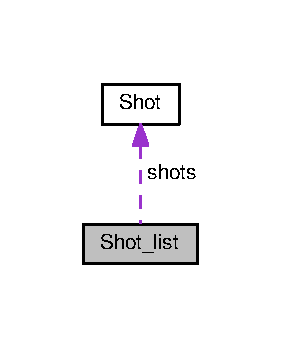
\includegraphics[width=136pt]{struct_shot__list__coll__graph}
\end{center}
\end{figure}
\subsection*{Data Fields}
\begin{DoxyCompactItemize}
\item 
int \hyperlink{struct_shot__list_a4276a0b800a4ef69dcbfeb381d1e7346}{shot\+\_\+count}
\item 
\hyperlink{struct_shot}{Shot} \hyperlink{struct_shot__list_a08606c51a264817a56f8af413248fa37}{shots} \mbox{[}S\+H\+O\+T\+\_\+\+M\+AX\mbox{]}
\end{DoxyCompactItemize}


\subsection{Detailed Description}
Objet contenant les informations pour un \hyperlink{struct_shot__list}{Shot\+\_\+list}. 

Objet contenant les informations pour un \hyperlink{struct_shot__list}{Shot\+\_\+list} int shot\+\_\+count; \hyperlink{struct_shot}{Shot} shots\mbox{[}S\+H\+O\+T\+\_\+\+M\+AX\mbox{]}; 

\subsection{Field Documentation}
\index{Shot\+\_\+list@{Shot\+\_\+list}!shot\+\_\+count@{shot\+\_\+count}}
\index{shot\+\_\+count@{shot\+\_\+count}!Shot\+\_\+list@{Shot\+\_\+list}}
\subsubsection[{\texorpdfstring{shot\+\_\+count}{shot_count}}]{\setlength{\rightskip}{0pt plus 5cm}int shot\+\_\+count}\hypertarget{struct_shot__list_a4276a0b800a4ef69dcbfeb381d1e7346}{}\label{struct_shot__list_a4276a0b800a4ef69dcbfeb381d1e7346}
Nombre de shot. \index{Shot\+\_\+list@{Shot\+\_\+list}!shots@{shots}}
\index{shots@{shots}!Shot\+\_\+list@{Shot\+\_\+list}}
\subsubsection[{\texorpdfstring{shots}{shots}}]{\setlength{\rightskip}{0pt plus 5cm}{\bf Shot} shots\mbox{[}S\+H\+O\+T\+\_\+\+M\+AX\mbox{]}}\hypertarget{struct_shot__list_a08606c51a264817a56f8af413248fa37}{}\label{struct_shot__list_a08606c51a264817a56f8af413248fa37}
Tableau de shots. 

The documentation for this struct was generated from the following file\+:\begin{DoxyCompactItemize}
\item 
\hyperlink{game_8h}{game.\+h}\end{DoxyCompactItemize}

\hypertarget{struct_track}{}\section{Track Struct Reference}
\label{struct_track}\index{Track@{Track}}


Objet contenant les informations pour un \hyperlink{struct_track}{Track}.  




{\ttfamily \#include $<$game.\+h$>$}



Collaboration diagram for Track\+:
\nopagebreak
\begin{figure}[H]
\begin{center}
\leavevmode
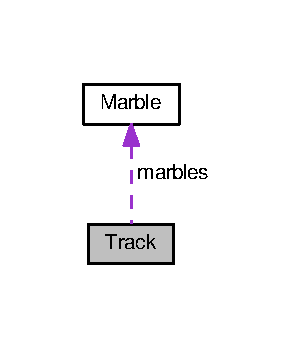
\includegraphics[width=141pt]{struct_track__coll__graph}
\end{center}
\end{figure}
\subsection*{Data Fields}
\begin{DoxyCompactItemize}
\item 
int \hyperlink{struct_track_a9e0d21871ffe556f58524ae0eab311b4}{sample\+\_\+count}
\item 
double \hyperlink{struct_track_aa3ed1a4220174d38001d02282fbee22b}{sample\+\_\+x} \mbox{[}S\+A\+M\+P\+L\+E\+\_\+\+M\+AX\mbox{]}
\item 
double \hyperlink{struct_track_a44edcc22cd2d982e8d90baa5aed0d36f}{sample\+\_\+y} \mbox{[}S\+A\+M\+P\+L\+E\+\_\+\+M\+AX\mbox{]}
\item 
int \hyperlink{struct_track_a59a42793ead243ec50ad584730b1fdab}{marble\+\_\+count}
\item 
int \hyperlink{struct_track_a5186ecb1e6c5695791274cd52cac839c}{first\+\_\+visible}
\item 
double \hyperlink{struct_track_a4acb65a6d65a7958036ed901abe0a6bb}{marbles\+\_\+speed}
\item 
\hyperlink{struct_marble}{Marble} \hyperlink{struct_track_a90e02a52ca50397997058e7b8dbab421}{marbles} \mbox{[}M\+A\+R\+B\+L\+E\+\_\+\+M\+AX\mbox{]}
\item 
\hyperlink{game_8h_a3d584d1e4b7b4c4a3cde3944c28fe594}{Track\+\_\+state} \hyperlink{struct_track_aadbac9f12492034fea9600a5ce4c7c5f}{state}
\end{DoxyCompactItemize}


\subsection{Detailed Description}
Objet contenant les informations pour un \hyperlink{struct_track}{Track}. 

Objet contenant les informations pour un \hyperlink{struct_track}{Track} int sample\+\_\+count; // échantillonnage courbe double sample\+\_\+x\mbox{[}S\+A\+M\+P\+L\+E\+\_\+\+M\+AX\mbox{]}, sample\+\_\+y\mbox{[}S\+A\+M\+P\+L\+E\+\_\+\+M\+AX\mbox{]}; int marble\+\_\+count; int first\+\_\+visible; double marbles\+\_\+speed; \hyperlink{struct_marble}{Marble} marbles\mbox{[}M\+A\+R\+B\+L\+E\+\_\+\+M\+AX\mbox{]}; Track\+\_\+state state; 

\subsection{Field Documentation}
\index{Track@{Track}!first\+\_\+visible@{first\+\_\+visible}}
\index{first\+\_\+visible@{first\+\_\+visible}!Track@{Track}}
\subsubsection[{\texorpdfstring{first\+\_\+visible}{first_visible}}]{\setlength{\rightskip}{0pt plus 5cm}int first\+\_\+visible}\hypertarget{struct_track_a5186ecb1e6c5695791274cd52cac839c}{}\label{struct_track_a5186ecb1e6c5695791274cd52cac839c}
Première bille visible. \index{Track@{Track}!marble\+\_\+count@{marble\+\_\+count}}
\index{marble\+\_\+count@{marble\+\_\+count}!Track@{Track}}
\subsubsection[{\texorpdfstring{marble\+\_\+count}{marble_count}}]{\setlength{\rightskip}{0pt plus 5cm}int marble\+\_\+count}\hypertarget{struct_track_a59a42793ead243ec50ad584730b1fdab}{}\label{struct_track_a59a42793ead243ec50ad584730b1fdab}
Nombre de marble. \index{Track@{Track}!marbles@{marbles}}
\index{marbles@{marbles}!Track@{Track}}
\subsubsection[{\texorpdfstring{marbles}{marbles}}]{\setlength{\rightskip}{0pt plus 5cm}{\bf Marble} marbles\mbox{[}M\+A\+R\+B\+L\+E\+\_\+\+M\+AX\mbox{]}}\hypertarget{struct_track_a90e02a52ca50397997058e7b8dbab421}{}\label{struct_track_a90e02a52ca50397997058e7b8dbab421}
Tableau de marble. \index{Track@{Track}!marbles\+\_\+speed@{marbles\+\_\+speed}}
\index{marbles\+\_\+speed@{marbles\+\_\+speed}!Track@{Track}}
\subsubsection[{\texorpdfstring{marbles\+\_\+speed}{marbles_speed}}]{\setlength{\rightskip}{0pt plus 5cm}double marbles\+\_\+speed}\hypertarget{struct_track_a4acb65a6d65a7958036ed901abe0a6bb}{}\label{struct_track_a4acb65a6d65a7958036ed901abe0a6bb}
Vitesse du train de bille. \index{Track@{Track}!sample\+\_\+count@{sample\+\_\+count}}
\index{sample\+\_\+count@{sample\+\_\+count}!Track@{Track}}
\subsubsection[{\texorpdfstring{sample\+\_\+count}{sample_count}}]{\setlength{\rightskip}{0pt plus 5cm}int sample\+\_\+count}\hypertarget{struct_track_a9e0d21871ffe556f58524ae0eab311b4}{}\label{struct_track_a9e0d21871ffe556f58524ae0eab311b4}
Échantillonnage courbe. \index{Track@{Track}!sample\+\_\+x@{sample\+\_\+x}}
\index{sample\+\_\+x@{sample\+\_\+x}!Track@{Track}}
\subsubsection[{\texorpdfstring{sample\+\_\+x}{sample_x}}]{\setlength{\rightskip}{0pt plus 5cm}double sample\+\_\+x\mbox{[}S\+A\+M\+P\+L\+E\+\_\+\+M\+AX\mbox{]}}\hypertarget{struct_track_aa3ed1a4220174d38001d02282fbee22b}{}\label{struct_track_aa3ed1a4220174d38001d02282fbee22b}
Sample\+\_\+x. \index{Track@{Track}!sample\+\_\+y@{sample\+\_\+y}}
\index{sample\+\_\+y@{sample\+\_\+y}!Track@{Track}}
\subsubsection[{\texorpdfstring{sample\+\_\+y}{sample_y}}]{\setlength{\rightskip}{0pt plus 5cm}double sample\+\_\+y\mbox{[}S\+A\+M\+P\+L\+E\+\_\+\+M\+AX\mbox{]}}\hypertarget{struct_track_a44edcc22cd2d982e8d90baa5aed0d36f}{}\label{struct_track_a44edcc22cd2d982e8d90baa5aed0d36f}
Sample\+\_\+y. \index{Track@{Track}!state@{state}}
\index{state@{state}!Track@{Track}}
\subsubsection[{\texorpdfstring{state}{state}}]{\setlength{\rightskip}{0pt plus 5cm}{\bf Track\+\_\+state} state}\hypertarget{struct_track_aadbac9f12492034fea9600a5ce4c7c5f}{}\label{struct_track_aadbac9f12492034fea9600a5ce4c7c5f}
État de la track. 

The documentation for this struct was generated from the following file\+:\begin{DoxyCompactItemize}
\item 
\hyperlink{game_8h}{game.\+h}\end{DoxyCompactItemize}

\hypertarget{struct_track__list}{}\section{Track\+\_\+list Struct Reference}
\label{struct_track__list}\index{Track\+\_\+list@{Track\+\_\+list}}


Objet contenant les informations pour un \hyperlink{struct_track__list}{Track\+\_\+list}.  




{\ttfamily \#include $<$game.\+h$>$}



Collaboration diagram for Track\+\_\+list\+:
\nopagebreak
\begin{figure}[H]
\begin{center}
\leavevmode
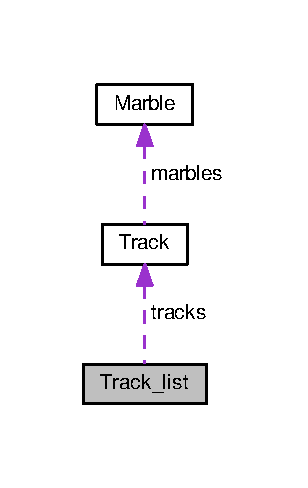
\includegraphics[width=148pt]{struct_track__list__coll__graph}
\end{center}
\end{figure}
\subsection*{Data Fields}
\begin{DoxyCompactItemize}
\item 
int \hyperlink{struct_track__list_ac955ea3b75270e8be80c62e8e6f4abc2}{track\+\_\+count}
\item 
\hyperlink{struct_track}{Track} \hyperlink{struct_track__list_a7c409b6c0307ab068387e40e51f139f9}{tracks} \mbox{[}T\+R\+A\+C\+K\+\_\+\+M\+AX\mbox{]}
\end{DoxyCompactItemize}


\subsection{Detailed Description}
Objet contenant les informations pour un \hyperlink{struct_track__list}{Track\+\_\+list}. 

Objet contenant les informations pour un \hyperlink{struct_track__list}{Track\+\_\+list}, actuellement une seules track est utilisé mais cette objet a été gardé afin de pouvoir gérer le multi-\/track facilement plus tard int track\+\_\+count; \hyperlink{struct_track}{Track} tracks\mbox{[}T\+R\+A\+C\+K\+\_\+\+M\+AX\mbox{]}; 

\subsection{Field Documentation}
\index{Track\+\_\+list@{Track\+\_\+list}!track\+\_\+count@{track\+\_\+count}}
\index{track\+\_\+count@{track\+\_\+count}!Track\+\_\+list@{Track\+\_\+list}}
\subsubsection[{\texorpdfstring{track\+\_\+count}{track_count}}]{\setlength{\rightskip}{0pt plus 5cm}int track\+\_\+count}\hypertarget{struct_track__list_ac955ea3b75270e8be80c62e8e6f4abc2}{}\label{struct_track__list_ac955ea3b75270e8be80c62e8e6f4abc2}
Nombre de track actuellement. \index{Track\+\_\+list@{Track\+\_\+list}!tracks@{tracks}}
\index{tracks@{tracks}!Track\+\_\+list@{Track\+\_\+list}}
\subsubsection[{\texorpdfstring{tracks}{tracks}}]{\setlength{\rightskip}{0pt plus 5cm}{\bf Track} tracks\mbox{[}T\+R\+A\+C\+K\+\_\+\+M\+AX\mbox{]}}\hypertarget{struct_track__list_a7c409b6c0307ab068387e40e51f139f9}{}\label{struct_track__list_a7c409b6c0307ab068387e40e51f139f9}
Liste des tracks. 

The documentation for this struct was generated from the following file\+:\begin{DoxyCompactItemize}
\item 
\hyperlink{game_8h}{game.\+h}\end{DoxyCompactItemize}

\chapter{File Documentation}
\hypertarget{curve_8c}{}\section{curve.\+c File Reference}
\label{curve_8c}\index{curve.\+c@{curve.\+c}}


Fonctions utiles de gestion des curves.  


{\ttfamily \#include $<$gtk/gtk.\+h$>$}\\*
{\ttfamily \#include $<$stdio.\+h$>$}\\*
{\ttfamily \#include $<$stdlib.\+h$>$}\\*
{\ttfamily \#include $<$string.\+h$>$}\\*
{\ttfamily \#include $<$math.\+h$>$}\\*
{\ttfamily \#include \char`\"{}util.\+h\char`\"{}}\\*
{\ttfamily \#include \char`\"{}curve.\+h\char`\"{}}\\*
Include dependency graph for curve.\+c\+:
\nopagebreak
\begin{figure}[H]
\begin{center}
\leavevmode
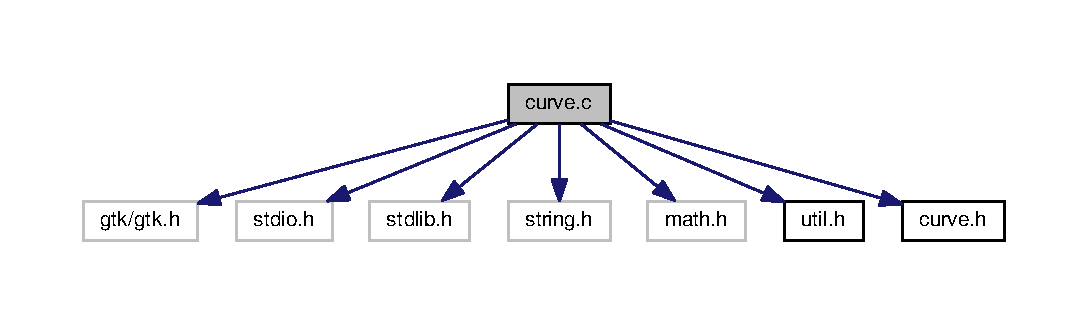
\includegraphics[width=350pt]{curve_8c__incl}
\end{center}
\end{figure}
\subsection*{Functions}
\begin{DoxyCompactItemize}
\item 
void \hyperlink{curve_8c_a3360cb91ca42b12fd7d2e3f5783c281e}{init\+\_\+curve\+\_\+infos} (\hyperlink{struct_curve__infos}{Curve\+\_\+infos} $\ast$ci)
\begin{DoxyCompactList}\small\item\em Fonction d\textquotesingle{}initialisation d\textquotesingle{}une \hyperlink{struct_curve__infos}{Curve\+\_\+infos}. \end{DoxyCompactList}\item 
int \hyperlink{curve_8c_a4382c60ac3b71f20fe1a04d4ae157e19}{add\+\_\+curve} (\hyperlink{struct_curve__infos}{Curve\+\_\+infos} $\ast$ci)
\begin{DoxyCompactList}\small\item\em Fonction d\textquotesingle{}ajout d\textquotesingle{}une courbe. \end{DoxyCompactList}\item 
int \hyperlink{curve_8c_a029fb6d4a949dd8a5885962ef644193b}{add\+\_\+control} (\hyperlink{struct_curve__infos}{Curve\+\_\+infos} $\ast$ci, double x, double y)
\begin{DoxyCompactList}\small\item\em Fonction d\textquotesingle{}ajout d\textquotesingle{}un point de control. \end{DoxyCompactList}\item 
int {\bfseries find\+\_\+control} (\hyperlink{struct_curve__infos}{Curve\+\_\+infos} $\ast$ci, double x, double y)\hypertarget{curve_8c_af035c1ad9b4ed42e612f475da2782373}{}\label{curve_8c_af035c1ad9b4ed42e612f475da2782373}

\item 
int {\bfseries move\+\_\+control} (\hyperlink{struct_curve__infos}{Curve\+\_\+infos} $\ast$ci, double dx, double dy)\hypertarget{curve_8c_a0c7b7ce869ee235d070a3f7866496729}{}\label{curve_8c_a0c7b7ce869ee235d070a3f7866496729}

\item 
int {\bfseries move\+\_\+curve} (\hyperlink{struct_curve__infos}{Curve\+\_\+infos} $\ast$ci, double dx, double dy)\hypertarget{curve_8c_af75239abce7bec98d2c05328e7ebc76e}{}\label{curve_8c_af75239abce7bec98d2c05328e7ebc76e}

\item 
int {\bfseries remove\+\_\+curve} (\hyperlink{struct_curve__infos}{Curve\+\_\+infos} $\ast$ci)\hypertarget{curve_8c_a693885879716f0332c7b63018992b377}{}\label{curve_8c_a693885879716f0332c7b63018992b377}

\item 
int {\bfseries remove\+\_\+control} (\hyperlink{struct_curve__infos}{Curve\+\_\+infos} $\ast$ci)\hypertarget{curve_8c_aa9e9c4adf064bfa7c9cb0be2a5ea895a}{}\label{curve_8c_aa9e9c4adf064bfa7c9cb0be2a5ea895a}

\item 
void {\bfseries convert\+\_\+bsp3\+\_\+to\+\_\+bezier} (double p\mbox{[}4\mbox{]}, double b\mbox{[}4\mbox{]})\hypertarget{curve_8c_ab4da14b153d5bfcb244e5826d397756b}{}\label{curve_8c_ab4da14b153d5bfcb244e5826d397756b}

\item 
void {\bfseries compute\+\_\+bezier\+\_\+points\+\_\+open} (\hyperlink{struct_curve}{Curve} $\ast$curve, int i, \hyperlink{struct_control}{Control} bez\+\_\+points\mbox{[}4\mbox{]})\hypertarget{curve_8c_a323d36be5a582f600d53874c81801237}{}\label{curve_8c_a323d36be5a582f600d53874c81801237}

\item 
void {\bfseries compute\+\_\+bezier\+\_\+points\+\_\+close} (\hyperlink{struct_curve}{Curve} $\ast$curve, int i, \hyperlink{struct_control}{Control} bez\+\_\+points\mbox{[}4\mbox{]})\hypertarget{curve_8c_a07d0d485848a23ab6c62d880dd48a88e}{}\label{curve_8c_a07d0d485848a23ab6c62d880dd48a88e}

\item 
double {\bfseries compute\+\_\+bezier\+\_\+cubic} (double b\mbox{[}4\mbox{]}, double t)\hypertarget{curve_8c_ad6a6784a9dfa5608a6aee1cbb6117c73}{}\label{curve_8c_ad6a6784a9dfa5608a6aee1cbb6117c73}

\item 
void {\bfseries convert\+\_\+bsp3\+\_\+to\+\_\+bezier\+\_\+prolong\+\_\+first} (double p\mbox{[}3\mbox{]}, double b\mbox{[}4\mbox{]})\hypertarget{curve_8c_a9b50fc3ffe4e0caeeb8ad24211f54635}{}\label{curve_8c_a9b50fc3ffe4e0caeeb8ad24211f54635}

\item 
void {\bfseries convert\+\_\+bsp3\+\_\+to\+\_\+bezier\+\_\+prolong\+\_\+last} (double p\mbox{[}3\mbox{]}, double b\mbox{[}4\mbox{]})\hypertarget{curve_8c_ad3b79dcebfd952c1424756c860d00d0a}{}\label{curve_8c_ad3b79dcebfd952c1424756c860d00d0a}

\item 
void {\bfseries compute\+\_\+bezier\+\_\+points\+\_\+prolong\+\_\+first} (\hyperlink{struct_curve}{Curve} $\ast$curve, \hyperlink{struct_control}{Control} bez\+\_\+points\mbox{[}4\mbox{]})\hypertarget{curve_8c_ac95630bb0745e2824af4cf8ac9b3dbca}{}\label{curve_8c_ac95630bb0745e2824af4cf8ac9b3dbca}

\item 
void {\bfseries compute\+\_\+bezier\+\_\+points\+\_\+prolong\+\_\+last} (\hyperlink{struct_curve}{Curve} $\ast$curve, \hyperlink{struct_control}{Control} bez\+\_\+points\mbox{[}4\mbox{]})\hypertarget{curve_8c_abf001f9d5caa6fdc25e8370386b9c86c}{}\label{curve_8c_abf001f9d5caa6fdc25e8370386b9c86c}

\item 
int {\bfseries move\+\_\+shift} (\hyperlink{struct_curve__infos}{Curve\+\_\+infos} $\ast$ci, double dx, double dy)\hypertarget{curve_8c_aaf7b43c9fb9beb3b65e4aa707b14487e}{}\label{curve_8c_aaf7b43c9fb9beb3b65e4aa707b14487e}

\item 
int {\bfseries reset\+\_\+shift} (\hyperlink{struct_curve__infos}{Curve\+\_\+infos} $\ast$ci)\hypertarget{curve_8c_a8842a21803607585a92e4eb18c0a85e8}{}\label{curve_8c_a8842a21803607585a92e4eb18c0a85e8}

\item 
void {\bfseries store\+\_\+sample} (double x, double y, double sx\mbox{[}$\,$\mbox{]}, double sy\mbox{[}$\,$\mbox{]}, int $\ast$ind, int ind\+\_\+max)\hypertarget{curve_8c_a5acc9f608ec71f57af12ed6da942b191}{}\label{curve_8c_a5acc9f608ec71f57af12ed6da942b191}

\item 
void {\bfseries sample\+\_\+bezier\+\_\+curve} (\hyperlink{struct_control}{Control} bez\+\_\+points\mbox{[}4\mbox{]}, double theta, double sx\mbox{[}$\,$\mbox{]}, double sy\mbox{[}$\,$\mbox{]}, int $\ast$ind, int ind\+\_\+max, int is\+\_\+first)\hypertarget{curve_8c_a7f14e0f14fe55ff9622939493fb826d0}{}\label{curve_8c_a7f14e0f14fe55ff9622939493fb826d0}

\item 
int {\bfseries interpolate\+\_\+samples} (double sx\mbox{[}$\,$\mbox{]}, double sy\mbox{[}$\,$\mbox{]}, double t, int tmax, double $\ast$x, double $\ast$y)\hypertarget{curve_8c_acf78e3306da0059ed6f578a106cd921f}{}\label{curve_8c_acf78e3306da0059ed6f578a106cd921f}

\item 
double \hyperlink{curve_8c_af0397016615860044c5f40372ceea7c0}{compute\+\_\+distant\+\_\+point\+\_\+forward} (double sx\mbox{[}$\,$\mbox{]}, double sy\mbox{[}$\,$\mbox{]}, double tA, int tmax, double dist, double $\ast$xB, double $\ast$yB)
\begin{DoxyCompactList}\small\item\em Fonction compute\+\_\+distant\+\_\+point\+\_\+forward. \end{DoxyCompactList}\item 
double \hyperlink{curve_8c_adc800d23a554aec2b7a807c6b722db69}{compute\+\_\+distant\+\_\+point\+\_\+backward} (double sx\mbox{[}$\,$\mbox{]}, double sy\mbox{[}$\,$\mbox{]}, double tA, int tmax, double dist, double $\ast$xB, double $\ast$yB)
\begin{DoxyCompactList}\small\item\em Fonction compute\+\_\+distant\+\_\+point\+\_\+backward. \end{DoxyCompactList}\item 
int \hyperlink{curve_8c_a0d17d6c7e9176239af44d6e0f9c68aab}{save\+\_\+curve\+\_\+to\+\_\+file} (\hyperlink{struct_curve__infos}{Curve\+\_\+infos} $\ast$ci, char $\ast$filename)
\begin{DoxyCompactList}\small\item\em Fonction de sauvegarde d\textquotesingle{}une curve infos dans un fichier .track. \end{DoxyCompactList}\item 
int \hyperlink{curve_8c_a6c3155460141faf83608fdde62bd18d1}{load\+\_\+curve\+\_\+from\+\_\+file} (\hyperlink{struct_curve__infos}{Curve\+\_\+infos} $\ast$ci, char $\ast$filename)
\begin{DoxyCompactList}\small\item\em Fonction de chargement d\textquotesingle{}une curve infos depuis un fichier .track. \end{DoxyCompactList}\end{DoxyCompactItemize}


\subsection{Detailed Description}
Fonctions utiles de gestion des curves. 

\begin{DoxyAuthor}{Author}
Gaëtan Perrot 
\end{DoxyAuthor}
\begin{DoxyVersion}{Version}
0.\+1 
\end{DoxyVersion}
\begin{DoxyDate}{Date}
23 avril 2017
\end{DoxyDate}
Fonctions utiles de gestion des curves 

\subsection{Function Documentation}
\index{curve.\+c@{curve.\+c}!add\+\_\+control@{add\+\_\+control}}
\index{add\+\_\+control@{add\+\_\+control}!curve.\+c@{curve.\+c}}
\subsubsection[{\texorpdfstring{add\+\_\+control(\+Curve\+\_\+infos $\ast$ci, double x, double y)}{add_control(Curve_infos *ci, double x, double y)}}]{\setlength{\rightskip}{0pt plus 5cm}int add\+\_\+control (
\begin{DoxyParamCaption}
\item[{{\bf Curve\+\_\+infos} $\ast$}]{ci, }
\item[{double}]{x, }
\item[{double}]{y}
\end{DoxyParamCaption}
)}\hypertarget{curve_8c_a029fb6d4a949dd8a5885962ef644193b}{}\label{curve_8c_a029fb6d4a949dd8a5885962ef644193b}


Fonction d\textquotesingle{}ajout d\textquotesingle{}un point de control. 


\begin{DoxyParams}{Parameters}
{\em self} & Objet \hyperlink{struct_curve__infos}{Curve\+\_\+infos}, double coordonnée x , double coordonnée y \\
\hline
\end{DoxyParams}
\begin{DoxyReturn}{Returns}
int nombre de point de control total 
\end{DoxyReturn}
\index{curve.\+c@{curve.\+c}!add\+\_\+curve@{add\+\_\+curve}}
\index{add\+\_\+curve@{add\+\_\+curve}!curve.\+c@{curve.\+c}}
\subsubsection[{\texorpdfstring{add\+\_\+curve(\+Curve\+\_\+infos $\ast$ci)}{add_curve(Curve_infos *ci)}}]{\setlength{\rightskip}{0pt plus 5cm}int add\+\_\+curve (
\begin{DoxyParamCaption}
\item[{{\bf Curve\+\_\+infos} $\ast$}]{ci}
\end{DoxyParamCaption}
)}\hypertarget{curve_8c_a4382c60ac3b71f20fe1a04d4ae157e19}{}\label{curve_8c_a4382c60ac3b71f20fe1a04d4ae157e19}


Fonction d\textquotesingle{}ajout d\textquotesingle{}une courbe. 


\begin{DoxyParams}{Parameters}
{\em self} & Objet \hyperlink{struct_curve__infos}{Curve\+\_\+infos} \\
\hline
\end{DoxyParams}
\begin{DoxyReturn}{Returns}
int nombre de courbe total 
\end{DoxyReturn}
\index{curve.\+c@{curve.\+c}!compute\+\_\+distant\+\_\+point\+\_\+backward@{compute\+\_\+distant\+\_\+point\+\_\+backward}}
\index{compute\+\_\+distant\+\_\+point\+\_\+backward@{compute\+\_\+distant\+\_\+point\+\_\+backward}!curve.\+c@{curve.\+c}}
\subsubsection[{\texorpdfstring{compute\+\_\+distant\+\_\+point\+\_\+backward(double sx[], double sy[], double t\+A, int tmax, double dist, double $\ast$x\+B, double $\ast$y\+B)}{compute_distant_point_backward(double sx[], double sy[], double tA, int tmax, double dist, double *xB, double *yB)}}]{\setlength{\rightskip}{0pt plus 5cm}double compute\+\_\+distant\+\_\+point\+\_\+backward (
\begin{DoxyParamCaption}
\item[{double}]{sx\mbox{[}$\,$\mbox{]}, }
\item[{double}]{sy\mbox{[}$\,$\mbox{]}, }
\item[{double}]{tA, }
\item[{int}]{tmax, }
\item[{double}]{dist, }
\item[{double $\ast$}]{xB, }
\item[{double $\ast$}]{yB}
\end{DoxyParamCaption}
)}\hypertarget{curve_8c_adc800d23a554aec2b7a807c6b722db69}{}\label{curve_8c_adc800d23a554aec2b7a807c6b722db69}


Fonction compute\+\_\+distant\+\_\+point\+\_\+backward. 


\begin{DoxyParams}{Parameters}
{\em self} & double sx\mbox{[}\mbox{]}, double sy\mbox{[}\mbox{]}, double tA, int tmax,double dist, double $\ast$xB, double $\ast$yB \\
\hline
\end{DoxyParams}
\begin{DoxyReturn}{Returns}
double 
\end{DoxyReturn}
\index{curve.\+c@{curve.\+c}!compute\+\_\+distant\+\_\+point\+\_\+forward@{compute\+\_\+distant\+\_\+point\+\_\+forward}}
\index{compute\+\_\+distant\+\_\+point\+\_\+forward@{compute\+\_\+distant\+\_\+point\+\_\+forward}!curve.\+c@{curve.\+c}}
\subsubsection[{\texorpdfstring{compute\+\_\+distant\+\_\+point\+\_\+forward(double sx[], double sy[], double t\+A, int tmax, double dist, double $\ast$x\+B, double $\ast$y\+B)}{compute_distant_point_forward(double sx[], double sy[], double tA, int tmax, double dist, double *xB, double *yB)}}]{\setlength{\rightskip}{0pt plus 5cm}double compute\+\_\+distant\+\_\+point\+\_\+forward (
\begin{DoxyParamCaption}
\item[{double}]{sx\mbox{[}$\,$\mbox{]}, }
\item[{double}]{sy\mbox{[}$\,$\mbox{]}, }
\item[{double}]{tA, }
\item[{int}]{tmax, }
\item[{double}]{dist, }
\item[{double $\ast$}]{xB, }
\item[{double $\ast$}]{yB}
\end{DoxyParamCaption}
)}\hypertarget{curve_8c_af0397016615860044c5f40372ceea7c0}{}\label{curve_8c_af0397016615860044c5f40372ceea7c0}


Fonction compute\+\_\+distant\+\_\+point\+\_\+forward. 


\begin{DoxyParams}{Parameters}
{\em self} & double sx\mbox{[}\mbox{]}, double sy\mbox{[}\mbox{]}, double tA, int tmax,double dist, double $\ast$xB, double $\ast$yB \\
\hline
\end{DoxyParams}
\begin{DoxyReturn}{Returns}
double 
\end{DoxyReturn}
\index{curve.\+c@{curve.\+c}!init\+\_\+curve\+\_\+infos@{init\+\_\+curve\+\_\+infos}}
\index{init\+\_\+curve\+\_\+infos@{init\+\_\+curve\+\_\+infos}!curve.\+c@{curve.\+c}}
\subsubsection[{\texorpdfstring{init\+\_\+curve\+\_\+infos(\+Curve\+\_\+infos $\ast$ci)}{init_curve_infos(Curve_infos *ci)}}]{\setlength{\rightskip}{0pt plus 5cm}void init\+\_\+curve\+\_\+infos (
\begin{DoxyParamCaption}
\item[{{\bf Curve\+\_\+infos} $\ast$}]{ci}
\end{DoxyParamCaption}
)}\hypertarget{curve_8c_a3360cb91ca42b12fd7d2e3f5783c281e}{}\label{curve_8c_a3360cb91ca42b12fd7d2e3f5783c281e}


Fonction d\textquotesingle{}initialisation d\textquotesingle{}une \hyperlink{struct_curve__infos}{Curve\+\_\+infos}. 


\begin{DoxyParams}{Parameters}
{\em self} & Objet \hyperlink{struct_curve__infos}{Curve\+\_\+infos} \\
\hline
\end{DoxyParams}
\begin{DoxyReturn}{Returns}
void 
\end{DoxyReturn}
\index{curve.\+c@{curve.\+c}!load\+\_\+curve\+\_\+from\+\_\+file@{load\+\_\+curve\+\_\+from\+\_\+file}}
\index{load\+\_\+curve\+\_\+from\+\_\+file@{load\+\_\+curve\+\_\+from\+\_\+file}!curve.\+c@{curve.\+c}}
\subsubsection[{\texorpdfstring{load\+\_\+curve\+\_\+from\+\_\+file(\+Curve\+\_\+infos $\ast$ci, char $\ast$filename)}{load_curve_from_file(Curve_infos *ci, char *filename)}}]{\setlength{\rightskip}{0pt plus 5cm}int load\+\_\+curve\+\_\+from\+\_\+file (
\begin{DoxyParamCaption}
\item[{{\bf Curve\+\_\+infos} $\ast$}]{ci, }
\item[{char $\ast$}]{filename}
\end{DoxyParamCaption}
)}\hypertarget{curve_8c_a6c3155460141faf83608fdde62bd18d1}{}\label{curve_8c_a6c3155460141faf83608fdde62bd18d1}


Fonction de chargement d\textquotesingle{}une curve infos depuis un fichier .track. 

Fonction pour tirer un shot.


\begin{DoxyParams}{Parameters}
{\em self} & Objet \hyperlink{struct_curve__infos}{Curve\+\_\+infos}, char $\ast$filename le nom du fichier \\
\hline
\end{DoxyParams}
\begin{DoxyReturn}{Returns}
int int retourne 1 si tout c\textquotesingle{}est bien passé et -\/1 si le chargement a échoué
\end{DoxyReturn}

\begin{DoxyParams}{Parameters}
{\em self} & Objet \hyperlink{struct_game}{Game} \\
\hline
\end{DoxyParams}
\begin{DoxyReturn}{Returns}
void 
\end{DoxyReturn}
\index{curve.\+c@{curve.\+c}!save\+\_\+curve\+\_\+to\+\_\+file@{save\+\_\+curve\+\_\+to\+\_\+file}}
\index{save\+\_\+curve\+\_\+to\+\_\+file@{save\+\_\+curve\+\_\+to\+\_\+file}!curve.\+c@{curve.\+c}}
\subsubsection[{\texorpdfstring{save\+\_\+curve\+\_\+to\+\_\+file(\+Curve\+\_\+infos $\ast$ci, char $\ast$filename)}{save_curve_to_file(Curve_infos *ci, char *filename)}}]{\setlength{\rightskip}{0pt plus 5cm}int save\+\_\+curve\+\_\+to\+\_\+file (
\begin{DoxyParamCaption}
\item[{{\bf Curve\+\_\+infos} $\ast$}]{ci, }
\item[{char $\ast$}]{filename}
\end{DoxyParamCaption}
)}\hypertarget{curve_8c_a0d17d6c7e9176239af44d6e0f9c68aab}{}\label{curve_8c_a0d17d6c7e9176239af44d6e0f9c68aab}


Fonction de sauvegarde d\textquotesingle{}une curve infos dans un fichier .track. 


\begin{DoxyParams}{Parameters}
{\em self} & Objet \hyperlink{struct_curve__infos}{Curve\+\_\+infos}, char $\ast$filename le nom du fichier \\
\hline
\end{DoxyParams}
\begin{DoxyReturn}{Returns}
int retourne 1 si tout c\textquotesingle{}est bien passé et -\/1 si la sauvegarde a échoué 
\end{DoxyReturn}

\hypertarget{curve_8h}{}\section{curve.\+h File Reference}
\label{curve_8h}\index{curve.\+h@{curve.\+h}}


Fonctions utiles de gestion des curves.  


This graph shows which files directly or indirectly include this file\+:
\nopagebreak
\begin{figure}[H]
\begin{center}
\leavevmode
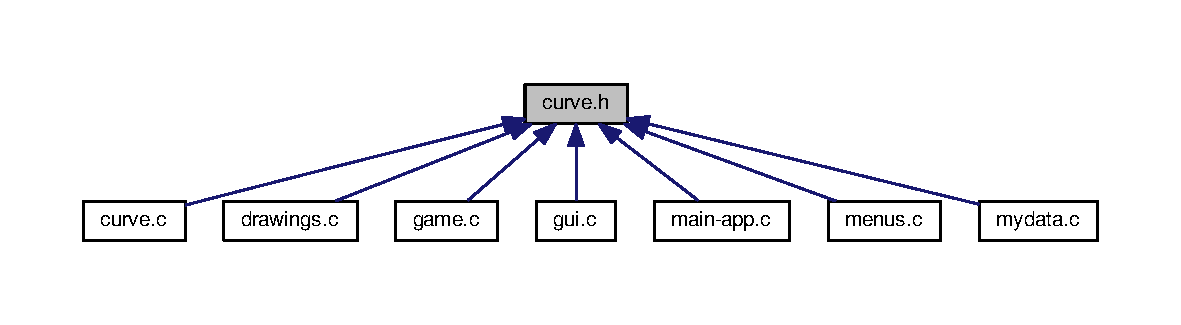
\includegraphics[width=350pt]{curve_8h__dep__incl}
\end{center}
\end{figure}
\subsection*{Data Structures}
\begin{DoxyCompactItemize}
\item 
struct \hyperlink{struct_control}{Control}
\begin{DoxyCompactList}\small\item\em Objet de point de control. \end{DoxyCompactList}\item 
struct \hyperlink{struct_curve}{Curve}
\begin{DoxyCompactList}\small\item\em Objet contenant une courbe. \end{DoxyCompactList}\item 
struct \hyperlink{struct_curve__list}{Curve\+\_\+list}
\begin{DoxyCompactList}\small\item\em Objet contenant un tableau de curve ainsi que le nombre de ces curves. \end{DoxyCompactList}\item 
struct \hyperlink{struct_curve__infos}{Curve\+\_\+infos}
\begin{DoxyCompactList}\small\item\em Objet contenant une curve\+\_\+list ainsi que la courbe courante et le point de control courant. \end{DoxyCompactList}\end{DoxyCompactItemize}
\subsection*{Macros}
\begin{DoxyCompactItemize}
\item 
\#define {\bfseries C\+O\+N\+T\+R\+O\+L\+\_\+\+M\+AX}~100\hypertarget{curve_8h_a813830b2e6d12ccb5196030749a197d1}{}\label{curve_8h_a813830b2e6d12ccb5196030749a197d1}

\item 
\#define {\bfseries C\+U\+R\+V\+E\+\_\+\+M\+AX}~200\hypertarget{curve_8h_a81902e9f1cd7055c09a56d55564d9221}{}\label{curve_8h_a81902e9f1cd7055c09a56d55564d9221}

\end{DoxyCompactItemize}
\subsection*{Functions}
\begin{DoxyCompactItemize}
\item 
void \hyperlink{curve_8h_a3360cb91ca42b12fd7d2e3f5783c281e}{init\+\_\+curve\+\_\+infos} (\hyperlink{struct_curve__infos}{Curve\+\_\+infos} $\ast$ci)
\begin{DoxyCompactList}\small\item\em Fonction d\textquotesingle{}initialisation d\textquotesingle{}une \hyperlink{struct_curve__infos}{Curve\+\_\+infos}. \end{DoxyCompactList}\item 
int \hyperlink{curve_8h_a4382c60ac3b71f20fe1a04d4ae157e19}{add\+\_\+curve} (\hyperlink{struct_curve__infos}{Curve\+\_\+infos} $\ast$ci)
\begin{DoxyCompactList}\small\item\em Fonction d\textquotesingle{}ajout d\textquotesingle{}une courbe. \end{DoxyCompactList}\item 
int \hyperlink{curve_8h_a029fb6d4a949dd8a5885962ef644193b}{add\+\_\+control} (\hyperlink{struct_curve__infos}{Curve\+\_\+infos} $\ast$ci, double x, double y)
\begin{DoxyCompactList}\small\item\em Fonction d\textquotesingle{}ajout d\textquotesingle{}un point de control. \end{DoxyCompactList}\item 
int {\bfseries find\+\_\+control} (\hyperlink{struct_curve__infos}{Curve\+\_\+infos} $\ast$ci, double x, double y)\hypertarget{curve_8h_af035c1ad9b4ed42e612f475da2782373}{}\label{curve_8h_af035c1ad9b4ed42e612f475da2782373}

\item 
int {\bfseries move\+\_\+control} (\hyperlink{struct_curve__infos}{Curve\+\_\+infos} $\ast$ci, double dx, double dy)\hypertarget{curve_8h_a0c7b7ce869ee235d070a3f7866496729}{}\label{curve_8h_a0c7b7ce869ee235d070a3f7866496729}

\item 
int {\bfseries move\+\_\+curve} (\hyperlink{struct_curve__infos}{Curve\+\_\+infos} $\ast$ci, double dx, double dy)\hypertarget{curve_8h_af75239abce7bec98d2c05328e7ebc76e}{}\label{curve_8h_af75239abce7bec98d2c05328e7ebc76e}

\item 
int {\bfseries remove\+\_\+curve} (\hyperlink{struct_curve__infos}{Curve\+\_\+infos} $\ast$ci)\hypertarget{curve_8h_a693885879716f0332c7b63018992b377}{}\label{curve_8h_a693885879716f0332c7b63018992b377}

\item 
int {\bfseries remove\+\_\+control} (\hyperlink{struct_curve__infos}{Curve\+\_\+infos} $\ast$ci)\hypertarget{curve_8h_aa9e9c4adf064bfa7c9cb0be2a5ea895a}{}\label{curve_8h_aa9e9c4adf064bfa7c9cb0be2a5ea895a}

\item 
void {\bfseries convert\+\_\+bsp3\+\_\+to\+\_\+bezier} (double p\mbox{[}4\mbox{]}, double b\mbox{[}4\mbox{]})\hypertarget{curve_8h_ab4da14b153d5bfcb244e5826d397756b}{}\label{curve_8h_ab4da14b153d5bfcb244e5826d397756b}

\item 
void {\bfseries compute\+\_\+bezier\+\_\+points\+\_\+open} (\hyperlink{struct_curve}{Curve} $\ast$curve, int i, \hyperlink{struct_control}{Control} bez\+\_\+points\mbox{[}4\mbox{]})\hypertarget{curve_8h_a323d36be5a582f600d53874c81801237}{}\label{curve_8h_a323d36be5a582f600d53874c81801237}

\item 
void {\bfseries compute\+\_\+bezier\+\_\+points\+\_\+close} (\hyperlink{struct_curve}{Curve} $\ast$curve, int i, \hyperlink{struct_control}{Control} bez\+\_\+points\mbox{[}4\mbox{]})\hypertarget{curve_8h_a07d0d485848a23ab6c62d880dd48a88e}{}\label{curve_8h_a07d0d485848a23ab6c62d880dd48a88e}

\item 
double {\bfseries compute\+\_\+bezier\+\_\+cubic} (double b\mbox{[}4\mbox{]}, double t)\hypertarget{curve_8h_ad6a6784a9dfa5608a6aee1cbb6117c73}{}\label{curve_8h_ad6a6784a9dfa5608a6aee1cbb6117c73}

\item 
void {\bfseries convert\+\_\+bsp3\+\_\+to\+\_\+bezier\+\_\+prolong\+\_\+first} (double p\mbox{[}3\mbox{]}, double b\mbox{[}4\mbox{]})\hypertarget{curve_8h_a9b50fc3ffe4e0caeeb8ad24211f54635}{}\label{curve_8h_a9b50fc3ffe4e0caeeb8ad24211f54635}

\item 
void {\bfseries convert\+\_\+bsp3\+\_\+to\+\_\+bezier\+\_\+prolong\+\_\+last} (double p\mbox{[}3\mbox{]}, double b\mbox{[}4\mbox{]})\hypertarget{curve_8h_ad3b79dcebfd952c1424756c860d00d0a}{}\label{curve_8h_ad3b79dcebfd952c1424756c860d00d0a}

\item 
void {\bfseries compute\+\_\+bezier\+\_\+points\+\_\+prolong\+\_\+first} (\hyperlink{struct_curve}{Curve} $\ast$curve, \hyperlink{struct_control}{Control} bez\+\_\+points\mbox{[}4\mbox{]})\hypertarget{curve_8h_ac95630bb0745e2824af4cf8ac9b3dbca}{}\label{curve_8h_ac95630bb0745e2824af4cf8ac9b3dbca}

\item 
void {\bfseries compute\+\_\+bezier\+\_\+points\+\_\+prolong\+\_\+last} (\hyperlink{struct_curve}{Curve} $\ast$curve, \hyperlink{struct_control}{Control} bez\+\_\+points\mbox{[}4\mbox{]})\hypertarget{curve_8h_abf001f9d5caa6fdc25e8370386b9c86c}{}\label{curve_8h_abf001f9d5caa6fdc25e8370386b9c86c}

\item 
int {\bfseries move\+\_\+shift} (\hyperlink{struct_curve__infos}{Curve\+\_\+infos} $\ast$ci, double dx, double dy)\hypertarget{curve_8h_aaf7b43c9fb9beb3b65e4aa707b14487e}{}\label{curve_8h_aaf7b43c9fb9beb3b65e4aa707b14487e}

\item 
int {\bfseries reset\+\_\+shift} (\hyperlink{struct_curve__infos}{Curve\+\_\+infos} $\ast$ci)\hypertarget{curve_8h_a8842a21803607585a92e4eb18c0a85e8}{}\label{curve_8h_a8842a21803607585a92e4eb18c0a85e8}

\item 
void {\bfseries store\+\_\+sample} (double x, double y, double sx\mbox{[}$\,$\mbox{]}, double sy\mbox{[}$\,$\mbox{]}, int $\ast$ind, int ind\+\_\+max)\hypertarget{curve_8h_a5acc9f608ec71f57af12ed6da942b191}{}\label{curve_8h_a5acc9f608ec71f57af12ed6da942b191}

\item 
void {\bfseries sample\+\_\+bezier\+\_\+curve} (\hyperlink{struct_control}{Control} bez\+\_\+points\mbox{[}4\mbox{]}, double theta, double sx\mbox{[}$\,$\mbox{]}, double sy\mbox{[}$\,$\mbox{]}, int $\ast$ind, int ind\+\_\+max, int is\+\_\+first)\hypertarget{curve_8h_a7f14e0f14fe55ff9622939493fb826d0}{}\label{curve_8h_a7f14e0f14fe55ff9622939493fb826d0}

\item 
int {\bfseries interpolate\+\_\+samples} (double sx\mbox{[}$\,$\mbox{]}, double sy\mbox{[}$\,$\mbox{]}, double t, int tmax, double $\ast$x, double $\ast$y)\hypertarget{curve_8h_acf78e3306da0059ed6f578a106cd921f}{}\label{curve_8h_acf78e3306da0059ed6f578a106cd921f}

\item 
double \hyperlink{curve_8h_af0397016615860044c5f40372ceea7c0}{compute\+\_\+distant\+\_\+point\+\_\+forward} (double sx\mbox{[}$\,$\mbox{]}, double sy\mbox{[}$\,$\mbox{]}, double tA, int tmax, double dist, double $\ast$xB, double $\ast$yB)
\begin{DoxyCompactList}\small\item\em Fonction compute\+\_\+distant\+\_\+point\+\_\+forward. \end{DoxyCompactList}\item 
double \hyperlink{curve_8h_adc800d23a554aec2b7a807c6b722db69}{compute\+\_\+distant\+\_\+point\+\_\+backward} (double sx\mbox{[}$\,$\mbox{]}, double sy\mbox{[}$\,$\mbox{]}, double tA, int tmax, double dist, double $\ast$xB, double $\ast$yB)
\begin{DoxyCompactList}\small\item\em Fonction compute\+\_\+distant\+\_\+point\+\_\+backward. \end{DoxyCompactList}\item 
int \hyperlink{curve_8h_a0d17d6c7e9176239af44d6e0f9c68aab}{save\+\_\+curve\+\_\+to\+\_\+file} (\hyperlink{struct_curve__infos}{Curve\+\_\+infos} $\ast$ci, char $\ast$filename)
\begin{DoxyCompactList}\small\item\em Fonction de sauvegarde d\textquotesingle{}une curve infos dans un fichier .track. \end{DoxyCompactList}\item 
int \hyperlink{curve_8h_a6c3155460141faf83608fdde62bd18d1}{load\+\_\+curve\+\_\+from\+\_\+file} (\hyperlink{struct_curve__infos}{Curve\+\_\+infos} $\ast$ci, char $\ast$filename)
\begin{DoxyCompactList}\small\item\em Fonction de chargement d\textquotesingle{}une curve infos depuis un fichier .track. \end{DoxyCompactList}\end{DoxyCompactItemize}


\subsection{Detailed Description}
Fonctions utiles de gestion des curves. 

\begin{DoxyAuthor}{Author}
Gaëtan Perrot 
\end{DoxyAuthor}
\begin{DoxyVersion}{Version}
0.\+1 
\end{DoxyVersion}
\begin{DoxyDate}{Date}
23 avril 2017
\end{DoxyDate}
Fonctions utiles de gestion des curves 

\subsection{Function Documentation}
\index{curve.\+h@{curve.\+h}!add\+\_\+control@{add\+\_\+control}}
\index{add\+\_\+control@{add\+\_\+control}!curve.\+h@{curve.\+h}}
\subsubsection[{\texorpdfstring{add\+\_\+control(\+Curve\+\_\+infos $\ast$ci, double x, double y)}{add_control(Curve_infos *ci, double x, double y)}}]{\setlength{\rightskip}{0pt plus 5cm}int add\+\_\+control (
\begin{DoxyParamCaption}
\item[{{\bf Curve\+\_\+infos} $\ast$}]{ci, }
\item[{double}]{x, }
\item[{double}]{y}
\end{DoxyParamCaption}
)}\hypertarget{curve_8h_a029fb6d4a949dd8a5885962ef644193b}{}\label{curve_8h_a029fb6d4a949dd8a5885962ef644193b}


Fonction d\textquotesingle{}ajout d\textquotesingle{}un point de control. 


\begin{DoxyParams}{Parameters}
{\em self} & Objet \hyperlink{struct_curve__infos}{Curve\+\_\+infos}, double coordonnée x , double coordonnée y \\
\hline
\end{DoxyParams}
\begin{DoxyReturn}{Returns}
int nombre de point de control total 
\end{DoxyReturn}
\index{curve.\+h@{curve.\+h}!add\+\_\+curve@{add\+\_\+curve}}
\index{add\+\_\+curve@{add\+\_\+curve}!curve.\+h@{curve.\+h}}
\subsubsection[{\texorpdfstring{add\+\_\+curve(\+Curve\+\_\+infos $\ast$ci)}{add_curve(Curve_infos *ci)}}]{\setlength{\rightskip}{0pt plus 5cm}int add\+\_\+curve (
\begin{DoxyParamCaption}
\item[{{\bf Curve\+\_\+infos} $\ast$}]{ci}
\end{DoxyParamCaption}
)}\hypertarget{curve_8h_a4382c60ac3b71f20fe1a04d4ae157e19}{}\label{curve_8h_a4382c60ac3b71f20fe1a04d4ae157e19}


Fonction d\textquotesingle{}ajout d\textquotesingle{}une courbe. 


\begin{DoxyParams}{Parameters}
{\em self} & Objet \hyperlink{struct_curve__infos}{Curve\+\_\+infos} \\
\hline
\end{DoxyParams}
\begin{DoxyReturn}{Returns}
int nombre de courbe total 
\end{DoxyReturn}
\index{curve.\+h@{curve.\+h}!compute\+\_\+distant\+\_\+point\+\_\+backward@{compute\+\_\+distant\+\_\+point\+\_\+backward}}
\index{compute\+\_\+distant\+\_\+point\+\_\+backward@{compute\+\_\+distant\+\_\+point\+\_\+backward}!curve.\+h@{curve.\+h}}
\subsubsection[{\texorpdfstring{compute\+\_\+distant\+\_\+point\+\_\+backward(double sx[], double sy[], double t\+A, int tmax, double dist, double $\ast$x\+B, double $\ast$y\+B)}{compute_distant_point_backward(double sx[], double sy[], double tA, int tmax, double dist, double *xB, double *yB)}}]{\setlength{\rightskip}{0pt plus 5cm}double compute\+\_\+distant\+\_\+point\+\_\+backward (
\begin{DoxyParamCaption}
\item[{double}]{sx\mbox{[}$\,$\mbox{]}, }
\item[{double}]{sy\mbox{[}$\,$\mbox{]}, }
\item[{double}]{tA, }
\item[{int}]{tmax, }
\item[{double}]{dist, }
\item[{double $\ast$}]{xB, }
\item[{double $\ast$}]{yB}
\end{DoxyParamCaption}
)}\hypertarget{curve_8h_adc800d23a554aec2b7a807c6b722db69}{}\label{curve_8h_adc800d23a554aec2b7a807c6b722db69}


Fonction compute\+\_\+distant\+\_\+point\+\_\+backward. 


\begin{DoxyParams}{Parameters}
{\em self} & double sx\mbox{[}\mbox{]}, double sy\mbox{[}\mbox{]}, double tA, int tmax,double dist, double $\ast$xB, double $\ast$yB \\
\hline
\end{DoxyParams}
\begin{DoxyReturn}{Returns}
double 
\end{DoxyReturn}
\index{curve.\+h@{curve.\+h}!compute\+\_\+distant\+\_\+point\+\_\+forward@{compute\+\_\+distant\+\_\+point\+\_\+forward}}
\index{compute\+\_\+distant\+\_\+point\+\_\+forward@{compute\+\_\+distant\+\_\+point\+\_\+forward}!curve.\+h@{curve.\+h}}
\subsubsection[{\texorpdfstring{compute\+\_\+distant\+\_\+point\+\_\+forward(double sx[], double sy[], double t\+A, int tmax, double dist, double $\ast$x\+B, double $\ast$y\+B)}{compute_distant_point_forward(double sx[], double sy[], double tA, int tmax, double dist, double *xB, double *yB)}}]{\setlength{\rightskip}{0pt plus 5cm}double compute\+\_\+distant\+\_\+point\+\_\+forward (
\begin{DoxyParamCaption}
\item[{double}]{sx\mbox{[}$\,$\mbox{]}, }
\item[{double}]{sy\mbox{[}$\,$\mbox{]}, }
\item[{double}]{tA, }
\item[{int}]{tmax, }
\item[{double}]{dist, }
\item[{double $\ast$}]{xB, }
\item[{double $\ast$}]{yB}
\end{DoxyParamCaption}
)}\hypertarget{curve_8h_af0397016615860044c5f40372ceea7c0}{}\label{curve_8h_af0397016615860044c5f40372ceea7c0}


Fonction compute\+\_\+distant\+\_\+point\+\_\+forward. 


\begin{DoxyParams}{Parameters}
{\em self} & double sx\mbox{[}\mbox{]}, double sy\mbox{[}\mbox{]}, double tA, int tmax,double dist, double $\ast$xB, double $\ast$yB \\
\hline
\end{DoxyParams}
\begin{DoxyReturn}{Returns}
double 
\end{DoxyReturn}
\index{curve.\+h@{curve.\+h}!init\+\_\+curve\+\_\+infos@{init\+\_\+curve\+\_\+infos}}
\index{init\+\_\+curve\+\_\+infos@{init\+\_\+curve\+\_\+infos}!curve.\+h@{curve.\+h}}
\subsubsection[{\texorpdfstring{init\+\_\+curve\+\_\+infos(\+Curve\+\_\+infos $\ast$ci)}{init_curve_infos(Curve_infos *ci)}}]{\setlength{\rightskip}{0pt plus 5cm}void init\+\_\+curve\+\_\+infos (
\begin{DoxyParamCaption}
\item[{{\bf Curve\+\_\+infos} $\ast$}]{ci}
\end{DoxyParamCaption}
)}\hypertarget{curve_8h_a3360cb91ca42b12fd7d2e3f5783c281e}{}\label{curve_8h_a3360cb91ca42b12fd7d2e3f5783c281e}


Fonction d\textquotesingle{}initialisation d\textquotesingle{}une \hyperlink{struct_curve__infos}{Curve\+\_\+infos}. 


\begin{DoxyParams}{Parameters}
{\em self} & Objet \hyperlink{struct_curve__infos}{Curve\+\_\+infos} \\
\hline
\end{DoxyParams}
\begin{DoxyReturn}{Returns}
void 
\end{DoxyReturn}
\index{curve.\+h@{curve.\+h}!load\+\_\+curve\+\_\+from\+\_\+file@{load\+\_\+curve\+\_\+from\+\_\+file}}
\index{load\+\_\+curve\+\_\+from\+\_\+file@{load\+\_\+curve\+\_\+from\+\_\+file}!curve.\+h@{curve.\+h}}
\subsubsection[{\texorpdfstring{load\+\_\+curve\+\_\+from\+\_\+file(\+Curve\+\_\+infos $\ast$ci, char $\ast$filename)}{load_curve_from_file(Curve_infos *ci, char *filename)}}]{\setlength{\rightskip}{0pt plus 5cm}int load\+\_\+curve\+\_\+from\+\_\+file (
\begin{DoxyParamCaption}
\item[{{\bf Curve\+\_\+infos} $\ast$}]{ci, }
\item[{char $\ast$}]{filename}
\end{DoxyParamCaption}
)}\hypertarget{curve_8h_a6c3155460141faf83608fdde62bd18d1}{}\label{curve_8h_a6c3155460141faf83608fdde62bd18d1}


Fonction de chargement d\textquotesingle{}une curve infos depuis un fichier .track. 

Fonction pour tirer un shot.


\begin{DoxyParams}{Parameters}
{\em self} & Objet \hyperlink{struct_curve__infos}{Curve\+\_\+infos}, char $\ast$filename le nom du fichier \\
\hline
\end{DoxyParams}
\begin{DoxyReturn}{Returns}
int int retourne 1 si tout c\textquotesingle{}est bien passé et -\/1 si le chargement a échoué
\end{DoxyReturn}

\begin{DoxyParams}{Parameters}
{\em self} & Objet \hyperlink{struct_game}{Game} \\
\hline
\end{DoxyParams}
\begin{DoxyReturn}{Returns}
void 
\end{DoxyReturn}
\index{curve.\+h@{curve.\+h}!save\+\_\+curve\+\_\+to\+\_\+file@{save\+\_\+curve\+\_\+to\+\_\+file}}
\index{save\+\_\+curve\+\_\+to\+\_\+file@{save\+\_\+curve\+\_\+to\+\_\+file}!curve.\+h@{curve.\+h}}
\subsubsection[{\texorpdfstring{save\+\_\+curve\+\_\+to\+\_\+file(\+Curve\+\_\+infos $\ast$ci, char $\ast$filename)}{save_curve_to_file(Curve_infos *ci, char *filename)}}]{\setlength{\rightskip}{0pt plus 5cm}int save\+\_\+curve\+\_\+to\+\_\+file (
\begin{DoxyParamCaption}
\item[{{\bf Curve\+\_\+infos} $\ast$}]{ci, }
\item[{char $\ast$}]{filename}
\end{DoxyParamCaption}
)}\hypertarget{curve_8h_a0d17d6c7e9176239af44d6e0f9c68aab}{}\label{curve_8h_a0d17d6c7e9176239af44d6e0f9c68aab}


Fonction de sauvegarde d\textquotesingle{}une curve infos dans un fichier .track. 


\begin{DoxyParams}{Parameters}
{\em self} & Objet \hyperlink{struct_curve__infos}{Curve\+\_\+infos}, char $\ast$filename le nom du fichier \\
\hline
\end{DoxyParams}
\begin{DoxyReturn}{Returns}
int retourne 1 si tout c\textquotesingle{}est bien passé et -\/1 si la sauvegarde a échoué 
\end{DoxyReturn}

\hypertarget{drawings_8c}{}\section{drawings.\+c File Reference}
\label{drawings_8c}\index{drawings.\+c@{drawings.\+c}}


Fonctions de dessin dans area avec cairo.  


{\ttfamily \#include $<$gtk/gtk.\+h$>$}\\*
{\ttfamily \#include $<$stdio.\+h$>$}\\*
{\ttfamily \#include $<$stdlib.\+h$>$}\\*
{\ttfamily \#include \char`\"{}util.\+h\char`\"{}}\\*
{\ttfamily \#include \char`\"{}curve.\+h\char`\"{}}\\*
{\ttfamily \#include \char`\"{}game.\+h\char`\"{}}\\*
{\ttfamily \#include \char`\"{}mydata.\+h\char`\"{}}\\*
{\ttfamily \#include \char`\"{}drawings.\+h\char`\"{}}\\*
{\ttfamily \#include \char`\"{}menus.\+h\char`\"{}}\\*
{\ttfamily \#include \char`\"{}font.\+h\char`\"{}}\\*
Include dependency graph for drawings.\+c\+:
\nopagebreak
\begin{figure}[H]
\begin{center}
\leavevmode
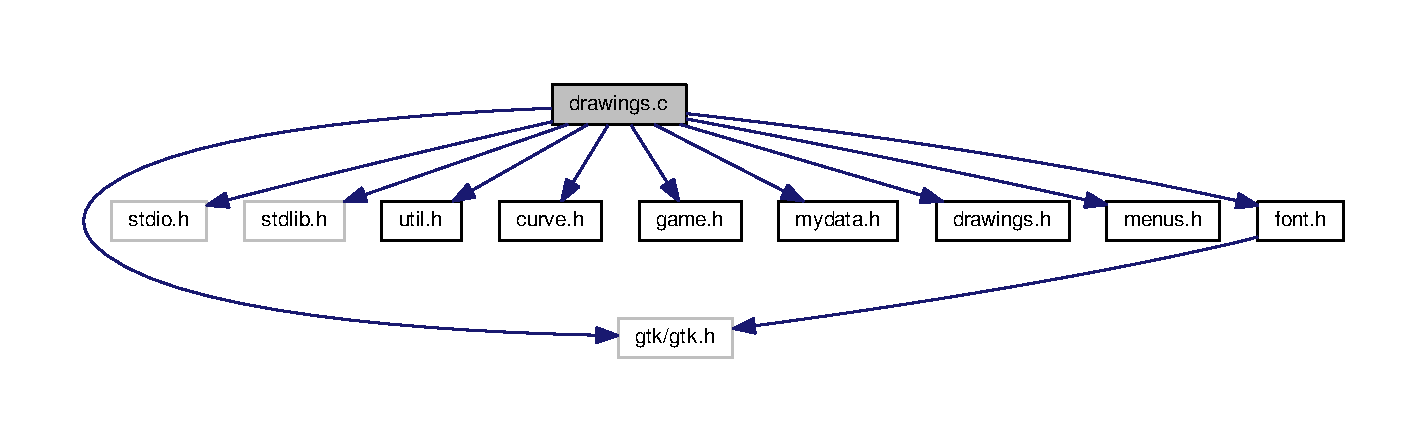
\includegraphics[width=350pt]{drawings_8c__incl}
\end{center}
\end{figure}
\subsection*{Functions}
\begin{DoxyCompactItemize}
\item 
gboolean {\bfseries on\+\_\+timeout} (gpointer data)\hypertarget{drawings_8c_abeaafffbc61bee0d635003ade901e0ce}{}\label{drawings_8c_abeaafffbc61bee0d635003ade901e0ce}

\item 
void {\bfseries apply\+\_\+image\+\_\+transforms} (\hyperlink{struct_mydata}{Mydata} $\ast$data)\hypertarget{drawings_8c_a1a60047a563d0f5ca7e51f78d25e6755}{}\label{drawings_8c_a1a60047a563d0f5ca7e51f78d25e6755}

\item 
void {\bfseries draw\+\_\+control\+\_\+polygons} (cairo\+\_\+t $\ast$cr, \hyperlink{struct_curve__infos}{Curve\+\_\+infos} $\ast$ci)\hypertarget{drawings_8c_aa2916387ed2bb46400a772edf5e5e482}{}\label{drawings_8c_aa2916387ed2bb46400a772edf5e5e482}

\item 
gboolean {\bfseries on\+\_\+area\+\_\+key\+\_\+press} (Gtk\+Widget $\ast$area, Gdk\+Event $\ast$event, gpointer data)\hypertarget{drawings_8c_a3f7aa1a6a60c2de908a231f8b753ce56}{}\label{drawings_8c_a3f7aa1a6a60c2de908a231f8b753ce56}

\item 
gboolean {\bfseries on\+\_\+area\+\_\+key\+\_\+release} (Gtk\+Widget $\ast$area, Gdk\+Event $\ast$event, gpointer data)\hypertarget{drawings_8c_a283df1e1e199997c3706485e0322281c}{}\label{drawings_8c_a283df1e1e199997c3706485e0322281c}

\item 
gboolean {\bfseries on\+\_\+area\+\_\+button\+\_\+press} (Gtk\+Widget $\ast$area, Gdk\+Event $\ast$event, gpointer data)\hypertarget{drawings_8c_af528da38bf7d80a4c73982b1c3b1aaec}{}\label{drawings_8c_af528da38bf7d80a4c73982b1c3b1aaec}

\item 
gboolean {\bfseries on\+\_\+area\+\_\+button\+\_\+release} (Gtk\+Widget $\ast$area, Gdk\+Event $\ast$event, gpointer data)\hypertarget{drawings_8c_ac3afd7a9454ebe3ed9f27d126638963a}{}\label{drawings_8c_ac3afd7a9454ebe3ed9f27d126638963a}

\item 
gboolean {\bfseries on\+\_\+area\+\_\+motion\+\_\+notify} (Gtk\+Widget $\ast$area, Gdk\+Event $\ast$event, gpointer data)\hypertarget{drawings_8c_a7dcb1b779674db2a800817d52d628d95}{}\label{drawings_8c_a7dcb1b779674db2a800817d52d628d95}

\item 
gboolean {\bfseries on\+\_\+area\+\_\+enter\+\_\+notify} (Gtk\+Widget $\ast$area, Gdk\+Event $\ast$event, gpointer data)\hypertarget{drawings_8c_a5002b23ba6d50a8952fa65c3aa925b19}{}\label{drawings_8c_a5002b23ba6d50a8952fa65c3aa925b19}

\item 
gboolean {\bfseries on\+\_\+area\+\_\+leave\+\_\+notify} (Gtk\+Widget $\ast$area, Gdk\+Event $\ast$event, gpointer data)\hypertarget{drawings_8c_ae5510e56cbdac869f39b1eba7fefe5d6}{}\label{drawings_8c_ae5510e56cbdac869f39b1eba7fefe5d6}

\item 
gboolean {\bfseries on\+\_\+area\+\_\+draw} (Gtk\+Widget $\ast$area, cairo\+\_\+t $\ast$cr, gpointer data)\hypertarget{drawings_8c_a67a7e2fd48a3328bcc90a5038d914acf}{}\label{drawings_8c_a67a7e2fd48a3328bcc90a5038d914acf}

\item 
gboolean {\bfseries on\+\_\+area\+\_\+resize\+\_\+window} (Gtk\+Widget $\ast$area, Gdk\+Event $\ast$event, gpointer data)\hypertarget{drawings_8c_a0a09ebf72544cf16711e3f01a44666e9}{}\label{drawings_8c_a0a09ebf72544cf16711e3f01a44666e9}

\item 
void {\bfseries draw\+\_\+control\+\_\+labels} (cairo\+\_\+t $\ast$cr, Pango\+Layout $\ast$layout, \hyperlink{struct_curve__infos}{Curve\+\_\+infos} $\ast$ci)\hypertarget{drawings_8c_a356bff98b57e38e6d000986d0c78d32a}{}\label{drawings_8c_a356bff98b57e38e6d000986d0c78d32a}

\item 
void {\bfseries draw\+\_\+bezier\+\_\+polygons\+\_\+open} (cairo\+\_\+t $\ast$cr, \hyperlink{struct_curve__infos}{Curve\+\_\+infos} $\ast$ci)\hypertarget{drawings_8c_a2367d9f272e9802dce9c2ccf6cb1b9cf}{}\label{drawings_8c_a2367d9f272e9802dce9c2ccf6cb1b9cf}

\item 
void {\bfseries draw\+\_\+bezier\+\_\+curve} (cairo\+\_\+t $\ast$cr, \hyperlink{struct_control}{Control} bez\+\_\+points\mbox{[}4\mbox{]}, double theta)\hypertarget{drawings_8c_affd3405db9cd4fb799cdc64177f45ebd}{}\label{drawings_8c_affd3405db9cd4fb799cdc64177f45ebd}

\item 
void {\bfseries draw\+\_\+bezier\+\_\+curves\+\_\+open} (cairo\+\_\+t $\ast$cr, \hyperlink{struct_curve__infos}{Curve\+\_\+infos} $\ast$ci, double theta)\hypertarget{drawings_8c_a5bd869742ca2d210d6d2d580e3039562}{}\label{drawings_8c_a5bd869742ca2d210d6d2d580e3039562}

\item 
void {\bfseries draw\+\_\+bezier\+\_\+curves\+\_\+close} (cairo\+\_\+t $\ast$cr, \hyperlink{struct_curve__infos}{Curve\+\_\+infos} $\ast$ci, double theta)\hypertarget{drawings_8c_a61156c2d248d68f486cd1c960a2a1956}{}\label{drawings_8c_a61156c2d248d68f486cd1c960a2a1956}

\item 
void {\bfseries draw\+\_\+bezier\+\_\+curves\+\_\+prolong} (cairo\+\_\+t $\ast$cr, \hyperlink{struct_curve__infos}{Curve\+\_\+infos} $\ast$ci, double theta)\hypertarget{drawings_8c_a5206bc4f02ad475ad780ee3db77e345b}{}\label{drawings_8c_a5206bc4f02ad475ad780ee3db77e345b}

\item 
void {\bfseries generate\+\_\+bezier\+\_\+path} (cairo\+\_\+t $\ast$cr, \hyperlink{struct_control}{Control} bez\+\_\+points\mbox{[}4\mbox{]}, double theta, int is\+\_\+first)\hypertarget{drawings_8c_afbfba3fd3a171ef4b9d8af2bb8572517}{}\label{drawings_8c_afbfba3fd3a171ef4b9d8af2bb8572517}

\item 
void {\bfseries draw\+\_\+bezier\+\_\+curves\+\_\+fill} (cairo\+\_\+t $\ast$cr, \hyperlink{struct_curve__infos}{Curve\+\_\+infos} $\ast$ci, double theta)\hypertarget{drawings_8c_af21c9cee4d112047d32486589245e096}{}\label{drawings_8c_af21c9cee4d112047d32486589245e096}

\item 
void {\bfseries draw\+\_\+bezier\+\_\+curves\+\_\+clip} (cairo\+\_\+t $\ast$cr, \hyperlink{struct_curve__infos}{Curve\+\_\+infos} $\ast$ci, double theta, \hyperlink{struct_mydata}{Mydata} $\ast$my)\hypertarget{drawings_8c_acb7155f40b67ccf7280b34d8d4e86531}{}\label{drawings_8c_acb7155f40b67ccf7280b34d8d4e86531}

\item 
void \hyperlink{drawings_8c_a5a8a7e187f959600594192cec54a578c}{switch\+\_\+shot\+\_\+color} (cairo\+\_\+t $\ast$cr, int color)
\begin{DoxyCompactList}\small\item\em Fonction pour choisir la couleur de dessin du cairo en fonction de la couleur de la bille. \end{DoxyCompactList}\item 
void \hyperlink{drawings_8c_af35ce069689e411753aa13938ef89a0f}{draw\+\_\+canon} (cairo\+\_\+t $\ast$cr, \hyperlink{struct_game}{Game} $\ast$game)
\begin{DoxyCompactList}\small\item\em Fonction d\textquotesingle{}affichage du canon. \end{DoxyCompactList}\item 
void \hyperlink{drawings_8c_adb57245779eb40b0a9111c7c5047f9e2}{draw\+\_\+shots} (cairo\+\_\+t $\ast$cr, \hyperlink{struct_game}{Game} $\ast$game)
\begin{DoxyCompactList}\small\item\em Fonction d\textquotesingle{}affichage des shots. \end{DoxyCompactList}\item 
void \hyperlink{drawings_8c_ab772221930486e28bf658267dfddf6a5}{draw\+\_\+track} (cairo\+\_\+t $\ast$cr, \hyperlink{struct_game}{Game} $\ast$game)
\begin{DoxyCompactList}\small\item\em Fonction d\textquotesingle{}affichage de la track. \end{DoxyCompactList}\item 
void \hyperlink{drawings_8c_af2d7c0359fb7530645b5a9c7db341920}{draw\+\_\+marbles\+\_\+bonus\+\_\+labels} (cairo\+\_\+t $\ast$cr, \hyperlink{struct_game}{Game} $\ast$game, Pango\+Layout $\ast$layout)
\begin{DoxyCompactList}\small\item\em Fonction d\textquotesingle{}affichage du label du bonus de la bille. \end{DoxyCompactList}\item 
void \hyperlink{drawings_8c_a44efb2de2c9e7ae7f7058629d4cea1e3}{draw\+\_\+marble} (cairo\+\_\+t $\ast$cr, \hyperlink{struct_marble}{Marble} $\ast$marble)
\begin{DoxyCompactList}\small\item\em Fonction d\textquotesingle{}affichage d\textquotesingle{}une bille. \end{DoxyCompactList}\item 
void \hyperlink{drawings_8c_a62bec0aefcaa2850956ab50fdbf84471}{draw\+\_\+marbles} (cairo\+\_\+t $\ast$cr, \hyperlink{struct_game}{Game} $\ast$game)
\begin{DoxyCompactList}\small\item\em Fonction d\textquotesingle{}affichage des billes. \end{DoxyCompactList}\item 
void \hyperlink{drawings_8c_acd9e48eb9bb11828e7914947853aad6e}{draw\+\_\+title} (\hyperlink{struct_mydata}{Mydata} $\ast$my, cairo\+\_\+t $\ast$cr)
\begin{DoxyCompactList}\small\item\em Fonction d\textquotesingle{}affichage de l\textquotesingle{}écran titre. \end{DoxyCompactList}\item 
void \hyperlink{drawings_8c_aa0efc5e769311ff5740f2f0208058598}{update\+\_\+\+Player\+\_\+\+Frame} (\hyperlink{struct_mydata}{Mydata} $\ast$my)
\begin{DoxyCompactList}\small\item\em Fonction de mise à jour du frame affichant les statistiques du joueur. \end{DoxyCompactList}\item 
void \hyperlink{drawings_8c_a1e81acf05d756f95b39b5be684ab9516}{game\+\_\+over\+\_\+message\+\_\+dialog} (gpointer data)
\begin{DoxyCompactList}\small\item\em Fonction de la fenêtre du gameover. \end{DoxyCompactList}\item 
void {\bfseries area\+\_\+init} (gpointer user\+\_\+data)\hypertarget{drawings_8c_a165f369e059a870a812e600f5b27e066}{}\label{drawings_8c_a165f369e059a870a812e600f5b27e066}

\end{DoxyCompactItemize}


\subsection{Detailed Description}
Fonctions de dessin dans area avec cairo. 

\begin{DoxyAuthor}{Author}
Gaëtan Perrot 
\end{DoxyAuthor}
\begin{DoxyVersion}{Version}
0.\+1 
\end{DoxyVersion}
\begin{DoxyDate}{Date}
23 avril 2017
\end{DoxyDate}
Fonctions de dessin dans area avec cairo 

\subsection{Function Documentation}
\index{drawings.\+c@{drawings.\+c}!draw\+\_\+canon@{draw\+\_\+canon}}
\index{draw\+\_\+canon@{draw\+\_\+canon}!drawings.\+c@{drawings.\+c}}
\subsubsection[{\texorpdfstring{draw\+\_\+canon(cairo\+\_\+t $\ast$cr, Game $\ast$game)}{draw_canon(cairo_t *cr, Game *game)}}]{\setlength{\rightskip}{0pt plus 5cm}void draw\+\_\+canon (
\begin{DoxyParamCaption}
\item[{cairo\+\_\+t $\ast$}]{cr, }
\item[{{\bf Game} $\ast$}]{game}
\end{DoxyParamCaption}
)}\hypertarget{drawings_8c_af35ce069689e411753aa13938ef89a0f}{}\label{drawings_8c_af35ce069689e411753aa13938ef89a0f}


Fonction d\textquotesingle{}affichage du canon. 


\begin{DoxyParams}{Parameters}
{\em self} & cairo\+\_\+t $\ast$cr, \hyperlink{struct_game}{Game} $\ast$ game \\
\hline
\end{DoxyParams}
\begin{DoxyReturn}{Returns}
void 
\end{DoxyReturn}
\index{drawings.\+c@{drawings.\+c}!draw\+\_\+marble@{draw\+\_\+marble}}
\index{draw\+\_\+marble@{draw\+\_\+marble}!drawings.\+c@{drawings.\+c}}
\subsubsection[{\texorpdfstring{draw\+\_\+marble(cairo\+\_\+t $\ast$cr, Marble $\ast$marble)}{draw_marble(cairo_t *cr, Marble *marble)}}]{\setlength{\rightskip}{0pt plus 5cm}void draw\+\_\+marble (
\begin{DoxyParamCaption}
\item[{cairo\+\_\+t $\ast$}]{cr, }
\item[{{\bf Marble} $\ast$}]{marble}
\end{DoxyParamCaption}
)}\hypertarget{drawings_8c_a44efb2de2c9e7ae7f7058629d4cea1e3}{}\label{drawings_8c_a44efb2de2c9e7ae7f7058629d4cea1e3}


Fonction d\textquotesingle{}affichage d\textquotesingle{}une bille. 


\begin{DoxyParams}{Parameters}
{\em self} & cairo\+\_\+t $\ast$cr, \hyperlink{struct_marble}{Marble} $\ast$ marble \\
\hline
\end{DoxyParams}
\begin{DoxyReturn}{Returns}
void 
\end{DoxyReturn}
\index{drawings.\+c@{drawings.\+c}!draw\+\_\+marbles@{draw\+\_\+marbles}}
\index{draw\+\_\+marbles@{draw\+\_\+marbles}!drawings.\+c@{drawings.\+c}}
\subsubsection[{\texorpdfstring{draw\+\_\+marbles(cairo\+\_\+t $\ast$cr, Game $\ast$game)}{draw_marbles(cairo_t *cr, Game *game)}}]{\setlength{\rightskip}{0pt plus 5cm}void draw\+\_\+marbles (
\begin{DoxyParamCaption}
\item[{cairo\+\_\+t $\ast$}]{cr, }
\item[{{\bf Game} $\ast$}]{game}
\end{DoxyParamCaption}
)}\hypertarget{drawings_8c_a62bec0aefcaa2850956ab50fdbf84471}{}\label{drawings_8c_a62bec0aefcaa2850956ab50fdbf84471}


Fonction d\textquotesingle{}affichage des billes. 


\begin{DoxyParams}{Parameters}
{\em self} & cairo\+\_\+t $\ast$cr, \hyperlink{struct_game}{Game} $\ast$ game \\
\hline
\end{DoxyParams}
\begin{DoxyReturn}{Returns}
void 
\end{DoxyReturn}
\index{drawings.\+c@{drawings.\+c}!draw\+\_\+marbles\+\_\+bonus\+\_\+labels@{draw\+\_\+marbles\+\_\+bonus\+\_\+labels}}
\index{draw\+\_\+marbles\+\_\+bonus\+\_\+labels@{draw\+\_\+marbles\+\_\+bonus\+\_\+labels}!drawings.\+c@{drawings.\+c}}
\subsubsection[{\texorpdfstring{draw\+\_\+marbles\+\_\+bonus\+\_\+labels(cairo\+\_\+t $\ast$cr, Game $\ast$game, Pango\+Layout $\ast$layout)}{draw_marbles_bonus_labels(cairo_t *cr, Game *game, PangoLayout *layout)}}]{\setlength{\rightskip}{0pt plus 5cm}void draw\+\_\+marbles\+\_\+bonus\+\_\+labels (
\begin{DoxyParamCaption}
\item[{cairo\+\_\+t $\ast$}]{cr, }
\item[{{\bf Game} $\ast$}]{game, }
\item[{Pango\+Layout $\ast$}]{layout}
\end{DoxyParamCaption}
)}\hypertarget{drawings_8c_af2d7c0359fb7530645b5a9c7db341920}{}\label{drawings_8c_af2d7c0359fb7530645b5a9c7db341920}


Fonction d\textquotesingle{}affichage du label du bonus de la bille. 


\begin{DoxyParams}{Parameters}
{\em self} & cairo\+\_\+t $\ast$cr, \hyperlink{struct_game}{Game} $\ast$ game,Pango\+Layout $\ast$layout \\
\hline
\end{DoxyParams}
\begin{DoxyReturn}{Returns}
void 
\end{DoxyReturn}
\index{drawings.\+c@{drawings.\+c}!draw\+\_\+shots@{draw\+\_\+shots}}
\index{draw\+\_\+shots@{draw\+\_\+shots}!drawings.\+c@{drawings.\+c}}
\subsubsection[{\texorpdfstring{draw\+\_\+shots(cairo\+\_\+t $\ast$cr, Game $\ast$game)}{draw_shots(cairo_t *cr, Game *game)}}]{\setlength{\rightskip}{0pt plus 5cm}void draw\+\_\+shots (
\begin{DoxyParamCaption}
\item[{cairo\+\_\+t $\ast$}]{cr, }
\item[{{\bf Game} $\ast$}]{game}
\end{DoxyParamCaption}
)}\hypertarget{drawings_8c_adb57245779eb40b0a9111c7c5047f9e2}{}\label{drawings_8c_adb57245779eb40b0a9111c7c5047f9e2}


Fonction d\textquotesingle{}affichage des shots. 


\begin{DoxyParams}{Parameters}
{\em self} & cairo\+\_\+t $\ast$cr, \hyperlink{struct_game}{Game} $\ast$ game \\
\hline
\end{DoxyParams}
\begin{DoxyReturn}{Returns}
void 
\end{DoxyReturn}
\index{drawings.\+c@{drawings.\+c}!draw\+\_\+title@{draw\+\_\+title}}
\index{draw\+\_\+title@{draw\+\_\+title}!drawings.\+c@{drawings.\+c}}
\subsubsection[{\texorpdfstring{draw\+\_\+title(\+Mydata $\ast$my, cairo\+\_\+t $\ast$cr)}{draw_title(Mydata *my, cairo_t *cr)}}]{\setlength{\rightskip}{0pt plus 5cm}void draw\+\_\+title (
\begin{DoxyParamCaption}
\item[{{\bf Mydata} $\ast$}]{my, }
\item[{cairo\+\_\+t $\ast$}]{cr}
\end{DoxyParamCaption}
)}\hypertarget{drawings_8c_acd9e48eb9bb11828e7914947853aad6e}{}\label{drawings_8c_acd9e48eb9bb11828e7914947853aad6e}


Fonction d\textquotesingle{}affichage de l\textquotesingle{}écran titre. 


\begin{DoxyParams}{Parameters}
{\em self} & \hyperlink{struct_mydata}{Mydata} $\ast$ my, cairo\+\_\+t $\ast$cr \\
\hline
\end{DoxyParams}
\begin{DoxyReturn}{Returns}
void 
\end{DoxyReturn}
\index{drawings.\+c@{drawings.\+c}!draw\+\_\+track@{draw\+\_\+track}}
\index{draw\+\_\+track@{draw\+\_\+track}!drawings.\+c@{drawings.\+c}}
\subsubsection[{\texorpdfstring{draw\+\_\+track(cairo\+\_\+t $\ast$cr, Game $\ast$game)}{draw_track(cairo_t *cr, Game *game)}}]{\setlength{\rightskip}{0pt plus 5cm}void draw\+\_\+track (
\begin{DoxyParamCaption}
\item[{cairo\+\_\+t $\ast$}]{cr, }
\item[{{\bf Game} $\ast$}]{game}
\end{DoxyParamCaption}
)}\hypertarget{drawings_8c_ab772221930486e28bf658267dfddf6a5}{}\label{drawings_8c_ab772221930486e28bf658267dfddf6a5}


Fonction d\textquotesingle{}affichage de la track. 


\begin{DoxyParams}{Parameters}
{\em self} & cairo\+\_\+t $\ast$cr, \hyperlink{struct_game}{Game} $\ast$ game \\
\hline
\end{DoxyParams}
\begin{DoxyReturn}{Returns}
void 
\end{DoxyReturn}
\index{drawings.\+c@{drawings.\+c}!game\+\_\+over\+\_\+message\+\_\+dialog@{game\+\_\+over\+\_\+message\+\_\+dialog}}
\index{game\+\_\+over\+\_\+message\+\_\+dialog@{game\+\_\+over\+\_\+message\+\_\+dialog}!drawings.\+c@{drawings.\+c}}
\subsubsection[{\texorpdfstring{game\+\_\+over\+\_\+message\+\_\+dialog(gpointer data)}{game_over_message_dialog(gpointer data)}}]{\setlength{\rightskip}{0pt plus 5cm}void game\+\_\+over\+\_\+message\+\_\+dialog (
\begin{DoxyParamCaption}
\item[{gpointer}]{data}
\end{DoxyParamCaption}
)}\hypertarget{drawings_8c_a1e81acf05d756f95b39b5be684ab9516}{}\label{drawings_8c_a1e81acf05d756f95b39b5be684ab9516}


Fonction de la fenêtre du gameover. 


\begin{DoxyParams}{Parameters}
{\em self} & gpointer objet \hyperlink{struct_mydata}{Mydata} \\
\hline
\end{DoxyParams}
\begin{DoxyReturn}{Returns}
void 
\end{DoxyReturn}
\index{drawings.\+c@{drawings.\+c}!switch\+\_\+shot\+\_\+color@{switch\+\_\+shot\+\_\+color}}
\index{switch\+\_\+shot\+\_\+color@{switch\+\_\+shot\+\_\+color}!drawings.\+c@{drawings.\+c}}
\subsubsection[{\texorpdfstring{switch\+\_\+shot\+\_\+color(cairo\+\_\+t $\ast$cr, int color)}{switch_shot_color(cairo_t *cr, int color)}}]{\setlength{\rightskip}{0pt plus 5cm}void switch\+\_\+shot\+\_\+color (
\begin{DoxyParamCaption}
\item[{cairo\+\_\+t $\ast$}]{cr, }
\item[{int}]{color}
\end{DoxyParamCaption}
)}\hypertarget{drawings_8c_a5a8a7e187f959600594192cec54a578c}{}\label{drawings_8c_a5a8a7e187f959600594192cec54a578c}


Fonction pour choisir la couleur de dessin du cairo en fonction de la couleur de la bille. 


\begin{DoxyParams}{Parameters}
{\em self} & cairo\+\_\+t $\ast$cr,int color \\
\hline
\end{DoxyParams}
\begin{DoxyReturn}{Returns}
void 
\end{DoxyReturn}
\index{drawings.\+c@{drawings.\+c}!update\+\_\+\+Player\+\_\+\+Frame@{update\+\_\+\+Player\+\_\+\+Frame}}
\index{update\+\_\+\+Player\+\_\+\+Frame@{update\+\_\+\+Player\+\_\+\+Frame}!drawings.\+c@{drawings.\+c}}
\subsubsection[{\texorpdfstring{update\+\_\+\+Player\+\_\+\+Frame(\+Mydata $\ast$my)}{update_Player_Frame(Mydata *my)}}]{\setlength{\rightskip}{0pt plus 5cm}void update\+\_\+\+Player\+\_\+\+Frame (
\begin{DoxyParamCaption}
\item[{{\bf Mydata} $\ast$}]{my}
\end{DoxyParamCaption}
)}\hypertarget{drawings_8c_aa0efc5e769311ff5740f2f0208058598}{}\label{drawings_8c_aa0efc5e769311ff5740f2f0208058598}


Fonction de mise à jour du frame affichant les statistiques du joueur. 


\begin{DoxyParams}{Parameters}
{\em self} & \hyperlink{struct_mydata}{Mydata} $\ast$ my \\
\hline
\end{DoxyParams}
\begin{DoxyReturn}{Returns}
void 
\end{DoxyReturn}

\hypertarget{drawings_8h}{}\section{drawings.\+h File Reference}
\label{drawings_8h}\index{drawings.\+h@{drawings.\+h}}


Fonctions de dessin dans area avec cairo.  


This graph shows which files directly or indirectly include this file\+:
\nopagebreak
\begin{figure}[H]
\begin{center}
\leavevmode
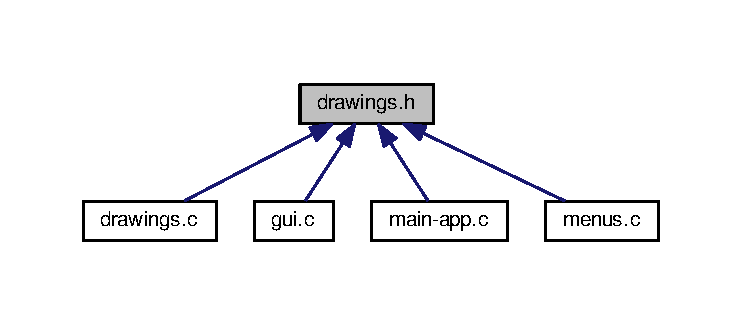
\includegraphics[width=350pt]{drawings_8h__dep__incl}
\end{center}
\end{figure}
\subsection*{Functions}
\begin{DoxyCompactItemize}
\item 
gboolean {\bfseries on\+\_\+timeout} (gpointer data)\hypertarget{drawings_8h_abeaafffbc61bee0d635003ade901e0ce}{}\label{drawings_8h_abeaafffbc61bee0d635003ade901e0ce}

\item 
void {\bfseries apply\+\_\+image\+\_\+transforms} (\hyperlink{struct_mydata}{Mydata} $\ast$data)\hypertarget{drawings_8h_a1a60047a563d0f5ca7e51f78d25e6755}{}\label{drawings_8h_a1a60047a563d0f5ca7e51f78d25e6755}

\item 
void {\bfseries draw\+\_\+curves} (cairo\+\_\+t $\ast$cr, \hyperlink{struct_curve__infos}{Curve\+\_\+infos} $\ast$ci)\hypertarget{drawings_8h_a6f7372befe6c29cb673352d00c2aef65}{}\label{drawings_8h_a6f7372befe6c29cb673352d00c2aef65}

\item 
void {\bfseries draw\+\_\+control\+\_\+labels} (cairo\+\_\+t $\ast$cr, Pango\+Layout $\ast$layout, \hyperlink{struct_curve__infos}{Curve\+\_\+infos} $\ast$ci)\hypertarget{drawings_8h_a356bff98b57e38e6d000986d0c78d32a}{}\label{drawings_8h_a356bff98b57e38e6d000986d0c78d32a}

\item 
void {\bfseries draw\+\_\+bezier\+\_\+polygons\+\_\+open} (cairo\+\_\+t $\ast$cr, \hyperlink{struct_curve__infos}{Curve\+\_\+infos} $\ast$ci)\hypertarget{drawings_8h_a2367d9f272e9802dce9c2ccf6cb1b9cf}{}\label{drawings_8h_a2367d9f272e9802dce9c2ccf6cb1b9cf}

\item 
void {\bfseries area\+\_\+init} (gpointer user\+\_\+data)\hypertarget{drawings_8h_a165f369e059a870a812e600f5b27e066}{}\label{drawings_8h_a165f369e059a870a812e600f5b27e066}

\item 
void {\bfseries draw\+\_\+bezier\+\_\+curve} (cairo\+\_\+t $\ast$cr, \hyperlink{struct_control}{Control} bez\+\_\+points\mbox{[}4\mbox{]}, double theta)\hypertarget{drawings_8h_affd3405db9cd4fb799cdc64177f45ebd}{}\label{drawings_8h_affd3405db9cd4fb799cdc64177f45ebd}

\item 
void {\bfseries draw\+\_\+bezier\+\_\+curves\+\_\+open} (cairo\+\_\+t $\ast$cr, \hyperlink{struct_curve__infos}{Curve\+\_\+infos} $\ast$ci, double theta)\hypertarget{drawings_8h_a5bd869742ca2d210d6d2d580e3039562}{}\label{drawings_8h_a5bd869742ca2d210d6d2d580e3039562}

\item 
void {\bfseries draw\+\_\+bezier\+\_\+curves\+\_\+close} (cairo\+\_\+t $\ast$cr, \hyperlink{struct_curve__infos}{Curve\+\_\+infos} $\ast$ci, double theta)\hypertarget{drawings_8h_a61156c2d248d68f486cd1c960a2a1956}{}\label{drawings_8h_a61156c2d248d68f486cd1c960a2a1956}

\item 
void {\bfseries draw\+\_\+bezier\+\_\+curves\+\_\+prolong} (cairo\+\_\+t $\ast$cr, \hyperlink{struct_curve__infos}{Curve\+\_\+infos} $\ast$ci, double theta)\hypertarget{drawings_8h_a5206bc4f02ad475ad780ee3db77e345b}{}\label{drawings_8h_a5206bc4f02ad475ad780ee3db77e345b}

\item 
void {\bfseries generate\+\_\+bezier\+\_\+path} (cairo\+\_\+t $\ast$cr, \hyperlink{struct_control}{Control} bez\+\_\+points\mbox{[}4\mbox{]}, double theta, int is\+\_\+first)\hypertarget{drawings_8h_afbfba3fd3a171ef4b9d8af2bb8572517}{}\label{drawings_8h_afbfba3fd3a171ef4b9d8af2bb8572517}

\item 
void \hyperlink{drawings_8h_a5a8a7e187f959600594192cec54a578c}{switch\+\_\+shot\+\_\+color} (cairo\+\_\+t $\ast$cr, int color)
\begin{DoxyCompactList}\small\item\em Fonction pour choisir la couleur de dessin du cairo en fonction de la couleur de la bille. \end{DoxyCompactList}\item 
void \hyperlink{drawings_8h_af35ce069689e411753aa13938ef89a0f}{draw\+\_\+canon} (cairo\+\_\+t $\ast$cr, \hyperlink{struct_game}{Game} $\ast$game)
\begin{DoxyCompactList}\small\item\em Fonction d\textquotesingle{}affichage du canon. \end{DoxyCompactList}\item 
void \hyperlink{drawings_8h_adb57245779eb40b0a9111c7c5047f9e2}{draw\+\_\+shots} (cairo\+\_\+t $\ast$cr, \hyperlink{struct_game}{Game} $\ast$game)
\begin{DoxyCompactList}\small\item\em Fonction d\textquotesingle{}affichage des shots. \end{DoxyCompactList}\item 
void \hyperlink{drawings_8h_ab772221930486e28bf658267dfddf6a5}{draw\+\_\+track} (cairo\+\_\+t $\ast$cr, \hyperlink{struct_game}{Game} $\ast$game)
\begin{DoxyCompactList}\small\item\em Fonction d\textquotesingle{}affichage de la track. \end{DoxyCompactList}\item 
void \hyperlink{drawings_8h_af2d7c0359fb7530645b5a9c7db341920}{draw\+\_\+marbles\+\_\+bonus\+\_\+labels} (cairo\+\_\+t $\ast$cr, \hyperlink{struct_game}{Game} $\ast$game, Pango\+Layout $\ast$layout)
\begin{DoxyCompactList}\small\item\em Fonction d\textquotesingle{}affichage du label du bonus de la bille. \end{DoxyCompactList}\item 
void \hyperlink{drawings_8h_a44efb2de2c9e7ae7f7058629d4cea1e3}{draw\+\_\+marble} (cairo\+\_\+t $\ast$cr, \hyperlink{struct_marble}{Marble} $\ast$marble)
\begin{DoxyCompactList}\small\item\em Fonction d\textquotesingle{}affichage d\textquotesingle{}une bille. \end{DoxyCompactList}\item 
void \hyperlink{drawings_8h_a62bec0aefcaa2850956ab50fdbf84471}{draw\+\_\+marbles} (cairo\+\_\+t $\ast$cr, \hyperlink{struct_game}{Game} $\ast$game)
\begin{DoxyCompactList}\small\item\em Fonction d\textquotesingle{}affichage des billes. \end{DoxyCompactList}\item 
void \hyperlink{drawings_8h_acd9e48eb9bb11828e7914947853aad6e}{draw\+\_\+title} (\hyperlink{struct_mydata}{Mydata} $\ast$my, cairo\+\_\+t $\ast$cr)
\begin{DoxyCompactList}\small\item\em Fonction d\textquotesingle{}affichage de l\textquotesingle{}écran titre. \end{DoxyCompactList}\item 
void \hyperlink{drawings_8h_aa0efc5e769311ff5740f2f0208058598}{update\+\_\+\+Player\+\_\+\+Frame} (\hyperlink{struct_mydata}{Mydata} $\ast$my)
\begin{DoxyCompactList}\small\item\em Fonction de mise à jour du frame affichant les statistiques du joueur. \end{DoxyCompactList}\item 
void \hyperlink{drawings_8h_a1e81acf05d756f95b39b5be684ab9516}{game\+\_\+over\+\_\+message\+\_\+dialog} (gpointer data)
\begin{DoxyCompactList}\small\item\em Fonction de la fenêtre du gameover. \end{DoxyCompactList}\end{DoxyCompactItemize}


\subsection{Detailed Description}
Fonctions de dessin dans area avec cairo. 

\begin{DoxyAuthor}{Author}
Gaëtan Perrot 
\end{DoxyAuthor}
\begin{DoxyVersion}{Version}
0.\+1 
\end{DoxyVersion}
\begin{DoxyDate}{Date}
23 avril 2017
\end{DoxyDate}
Fonctions de dessin dans area avec cairo 

\subsection{Function Documentation}
\index{drawings.\+h@{drawings.\+h}!draw\+\_\+canon@{draw\+\_\+canon}}
\index{draw\+\_\+canon@{draw\+\_\+canon}!drawings.\+h@{drawings.\+h}}
\subsubsection[{\texorpdfstring{draw\+\_\+canon(cairo\+\_\+t $\ast$cr, Game $\ast$game)}{draw_canon(cairo_t *cr, Game *game)}}]{\setlength{\rightskip}{0pt plus 5cm}void draw\+\_\+canon (
\begin{DoxyParamCaption}
\item[{cairo\+\_\+t $\ast$}]{cr, }
\item[{{\bf Game} $\ast$}]{game}
\end{DoxyParamCaption}
)}\hypertarget{drawings_8h_af35ce069689e411753aa13938ef89a0f}{}\label{drawings_8h_af35ce069689e411753aa13938ef89a0f}


Fonction d\textquotesingle{}affichage du canon. 


\begin{DoxyParams}{Parameters}
{\em self} & cairo\+\_\+t $\ast$cr, \hyperlink{struct_game}{Game} $\ast$ game \\
\hline
\end{DoxyParams}
\begin{DoxyReturn}{Returns}
void 
\end{DoxyReturn}
\index{drawings.\+h@{drawings.\+h}!draw\+\_\+marble@{draw\+\_\+marble}}
\index{draw\+\_\+marble@{draw\+\_\+marble}!drawings.\+h@{drawings.\+h}}
\subsubsection[{\texorpdfstring{draw\+\_\+marble(cairo\+\_\+t $\ast$cr, Marble $\ast$marble)}{draw_marble(cairo_t *cr, Marble *marble)}}]{\setlength{\rightskip}{0pt plus 5cm}void draw\+\_\+marble (
\begin{DoxyParamCaption}
\item[{cairo\+\_\+t $\ast$}]{cr, }
\item[{{\bf Marble} $\ast$}]{marble}
\end{DoxyParamCaption}
)}\hypertarget{drawings_8h_a44efb2de2c9e7ae7f7058629d4cea1e3}{}\label{drawings_8h_a44efb2de2c9e7ae7f7058629d4cea1e3}


Fonction d\textquotesingle{}affichage d\textquotesingle{}une bille. 


\begin{DoxyParams}{Parameters}
{\em self} & cairo\+\_\+t $\ast$cr, \hyperlink{struct_marble}{Marble} $\ast$ marble \\
\hline
\end{DoxyParams}
\begin{DoxyReturn}{Returns}
void 
\end{DoxyReturn}
\index{drawings.\+h@{drawings.\+h}!draw\+\_\+marbles@{draw\+\_\+marbles}}
\index{draw\+\_\+marbles@{draw\+\_\+marbles}!drawings.\+h@{drawings.\+h}}
\subsubsection[{\texorpdfstring{draw\+\_\+marbles(cairo\+\_\+t $\ast$cr, Game $\ast$game)}{draw_marbles(cairo_t *cr, Game *game)}}]{\setlength{\rightskip}{0pt plus 5cm}void draw\+\_\+marbles (
\begin{DoxyParamCaption}
\item[{cairo\+\_\+t $\ast$}]{cr, }
\item[{{\bf Game} $\ast$}]{game}
\end{DoxyParamCaption}
)}\hypertarget{drawings_8h_a62bec0aefcaa2850956ab50fdbf84471}{}\label{drawings_8h_a62bec0aefcaa2850956ab50fdbf84471}


Fonction d\textquotesingle{}affichage des billes. 


\begin{DoxyParams}{Parameters}
{\em self} & cairo\+\_\+t $\ast$cr, \hyperlink{struct_game}{Game} $\ast$ game \\
\hline
\end{DoxyParams}
\begin{DoxyReturn}{Returns}
void 
\end{DoxyReturn}
\index{drawings.\+h@{drawings.\+h}!draw\+\_\+marbles\+\_\+bonus\+\_\+labels@{draw\+\_\+marbles\+\_\+bonus\+\_\+labels}}
\index{draw\+\_\+marbles\+\_\+bonus\+\_\+labels@{draw\+\_\+marbles\+\_\+bonus\+\_\+labels}!drawings.\+h@{drawings.\+h}}
\subsubsection[{\texorpdfstring{draw\+\_\+marbles\+\_\+bonus\+\_\+labels(cairo\+\_\+t $\ast$cr, Game $\ast$game, Pango\+Layout $\ast$layout)}{draw_marbles_bonus_labels(cairo_t *cr, Game *game, PangoLayout *layout)}}]{\setlength{\rightskip}{0pt plus 5cm}void draw\+\_\+marbles\+\_\+bonus\+\_\+labels (
\begin{DoxyParamCaption}
\item[{cairo\+\_\+t $\ast$}]{cr, }
\item[{{\bf Game} $\ast$}]{game, }
\item[{Pango\+Layout $\ast$}]{layout}
\end{DoxyParamCaption}
)}\hypertarget{drawings_8h_af2d7c0359fb7530645b5a9c7db341920}{}\label{drawings_8h_af2d7c0359fb7530645b5a9c7db341920}


Fonction d\textquotesingle{}affichage du label du bonus de la bille. 


\begin{DoxyParams}{Parameters}
{\em self} & cairo\+\_\+t $\ast$cr, \hyperlink{struct_game}{Game} $\ast$ game,Pango\+Layout $\ast$layout \\
\hline
\end{DoxyParams}
\begin{DoxyReturn}{Returns}
void 
\end{DoxyReturn}
\index{drawings.\+h@{drawings.\+h}!draw\+\_\+shots@{draw\+\_\+shots}}
\index{draw\+\_\+shots@{draw\+\_\+shots}!drawings.\+h@{drawings.\+h}}
\subsubsection[{\texorpdfstring{draw\+\_\+shots(cairo\+\_\+t $\ast$cr, Game $\ast$game)}{draw_shots(cairo_t *cr, Game *game)}}]{\setlength{\rightskip}{0pt plus 5cm}void draw\+\_\+shots (
\begin{DoxyParamCaption}
\item[{cairo\+\_\+t $\ast$}]{cr, }
\item[{{\bf Game} $\ast$}]{game}
\end{DoxyParamCaption}
)}\hypertarget{drawings_8h_adb57245779eb40b0a9111c7c5047f9e2}{}\label{drawings_8h_adb57245779eb40b0a9111c7c5047f9e2}


Fonction d\textquotesingle{}affichage des shots. 


\begin{DoxyParams}{Parameters}
{\em self} & cairo\+\_\+t $\ast$cr, \hyperlink{struct_game}{Game} $\ast$ game \\
\hline
\end{DoxyParams}
\begin{DoxyReturn}{Returns}
void 
\end{DoxyReturn}
\index{drawings.\+h@{drawings.\+h}!draw\+\_\+title@{draw\+\_\+title}}
\index{draw\+\_\+title@{draw\+\_\+title}!drawings.\+h@{drawings.\+h}}
\subsubsection[{\texorpdfstring{draw\+\_\+title(\+Mydata $\ast$my, cairo\+\_\+t $\ast$cr)}{draw_title(Mydata *my, cairo_t *cr)}}]{\setlength{\rightskip}{0pt plus 5cm}void draw\+\_\+title (
\begin{DoxyParamCaption}
\item[{{\bf Mydata} $\ast$}]{my, }
\item[{cairo\+\_\+t $\ast$}]{cr}
\end{DoxyParamCaption}
)}\hypertarget{drawings_8h_acd9e48eb9bb11828e7914947853aad6e}{}\label{drawings_8h_acd9e48eb9bb11828e7914947853aad6e}


Fonction d\textquotesingle{}affichage de l\textquotesingle{}écran titre. 


\begin{DoxyParams}{Parameters}
{\em self} & \hyperlink{struct_mydata}{Mydata} $\ast$ my, cairo\+\_\+t $\ast$cr \\
\hline
\end{DoxyParams}
\begin{DoxyReturn}{Returns}
void 
\end{DoxyReturn}
\index{drawings.\+h@{drawings.\+h}!draw\+\_\+track@{draw\+\_\+track}}
\index{draw\+\_\+track@{draw\+\_\+track}!drawings.\+h@{drawings.\+h}}
\subsubsection[{\texorpdfstring{draw\+\_\+track(cairo\+\_\+t $\ast$cr, Game $\ast$game)}{draw_track(cairo_t *cr, Game *game)}}]{\setlength{\rightskip}{0pt plus 5cm}void draw\+\_\+track (
\begin{DoxyParamCaption}
\item[{cairo\+\_\+t $\ast$}]{cr, }
\item[{{\bf Game} $\ast$}]{game}
\end{DoxyParamCaption}
)}\hypertarget{drawings_8h_ab772221930486e28bf658267dfddf6a5}{}\label{drawings_8h_ab772221930486e28bf658267dfddf6a5}


Fonction d\textquotesingle{}affichage de la track. 


\begin{DoxyParams}{Parameters}
{\em self} & cairo\+\_\+t $\ast$cr, \hyperlink{struct_game}{Game} $\ast$ game \\
\hline
\end{DoxyParams}
\begin{DoxyReturn}{Returns}
void 
\end{DoxyReturn}
\index{drawings.\+h@{drawings.\+h}!game\+\_\+over\+\_\+message\+\_\+dialog@{game\+\_\+over\+\_\+message\+\_\+dialog}}
\index{game\+\_\+over\+\_\+message\+\_\+dialog@{game\+\_\+over\+\_\+message\+\_\+dialog}!drawings.\+h@{drawings.\+h}}
\subsubsection[{\texorpdfstring{game\+\_\+over\+\_\+message\+\_\+dialog(gpointer data)}{game_over_message_dialog(gpointer data)}}]{\setlength{\rightskip}{0pt plus 5cm}void game\+\_\+over\+\_\+message\+\_\+dialog (
\begin{DoxyParamCaption}
\item[{gpointer}]{data}
\end{DoxyParamCaption}
)}\hypertarget{drawings_8h_a1e81acf05d756f95b39b5be684ab9516}{}\label{drawings_8h_a1e81acf05d756f95b39b5be684ab9516}


Fonction de la fenêtre du gameover. 


\begin{DoxyParams}{Parameters}
{\em self} & gpointer objet \hyperlink{struct_mydata}{Mydata} \\
\hline
\end{DoxyParams}
\begin{DoxyReturn}{Returns}
void 
\end{DoxyReturn}
\index{drawings.\+h@{drawings.\+h}!switch\+\_\+shot\+\_\+color@{switch\+\_\+shot\+\_\+color}}
\index{switch\+\_\+shot\+\_\+color@{switch\+\_\+shot\+\_\+color}!drawings.\+h@{drawings.\+h}}
\subsubsection[{\texorpdfstring{switch\+\_\+shot\+\_\+color(cairo\+\_\+t $\ast$cr, int color)}{switch_shot_color(cairo_t *cr, int color)}}]{\setlength{\rightskip}{0pt plus 5cm}void switch\+\_\+shot\+\_\+color (
\begin{DoxyParamCaption}
\item[{cairo\+\_\+t $\ast$}]{cr, }
\item[{int}]{color}
\end{DoxyParamCaption}
)}\hypertarget{drawings_8h_a5a8a7e187f959600594192cec54a578c}{}\label{drawings_8h_a5a8a7e187f959600594192cec54a578c}


Fonction pour choisir la couleur de dessin du cairo en fonction de la couleur de la bille. 


\begin{DoxyParams}{Parameters}
{\em self} & cairo\+\_\+t $\ast$cr,int color \\
\hline
\end{DoxyParams}
\begin{DoxyReturn}{Returns}
void 
\end{DoxyReturn}
\index{drawings.\+h@{drawings.\+h}!update\+\_\+\+Player\+\_\+\+Frame@{update\+\_\+\+Player\+\_\+\+Frame}}
\index{update\+\_\+\+Player\+\_\+\+Frame@{update\+\_\+\+Player\+\_\+\+Frame}!drawings.\+h@{drawings.\+h}}
\subsubsection[{\texorpdfstring{update\+\_\+\+Player\+\_\+\+Frame(\+Mydata $\ast$my)}{update_Player_Frame(Mydata *my)}}]{\setlength{\rightskip}{0pt plus 5cm}void update\+\_\+\+Player\+\_\+\+Frame (
\begin{DoxyParamCaption}
\item[{{\bf Mydata} $\ast$}]{my}
\end{DoxyParamCaption}
)}\hypertarget{drawings_8h_aa0efc5e769311ff5740f2f0208058598}{}\label{drawings_8h_aa0efc5e769311ff5740f2f0208058598}


Fonction de mise à jour du frame affichant les statistiques du joueur. 


\begin{DoxyParams}{Parameters}
{\em self} & \hyperlink{struct_mydata}{Mydata} $\ast$ my \\
\hline
\end{DoxyParams}
\begin{DoxyReturn}{Returns}
void 
\end{DoxyReturn}

\hypertarget{game_8c}{}\section{game.\+c File Reference}
\label{game_8c}\index{game.\+c@{game.\+c}}


Fonctions et objets principaux du jeu.  


{\ttfamily \#include $<$gtk/gtk.\+h$>$}\\*
{\ttfamily \#include $<$stdio.\+h$>$}\\*
{\ttfamily \#include $<$stdlib.\+h$>$}\\*
{\ttfamily \#include $<$math.\+h$>$}\\*
{\ttfamily \#include $<$time.\+h$>$}\\*
{\ttfamily \#include $<$string.\+h$>$}\\*
{\ttfamily \#include \char`\"{}curve.\+h\char`\"{}}\\*
{\ttfamily \#include \char`\"{}game.\+h\char`\"{}}\\*
{\ttfamily \#include \char`\"{}util.\+h\char`\"{}}\\*
Include dependency graph for game.\+c\+:
\nopagebreak
\begin{figure}[H]
\begin{center}
\leavevmode
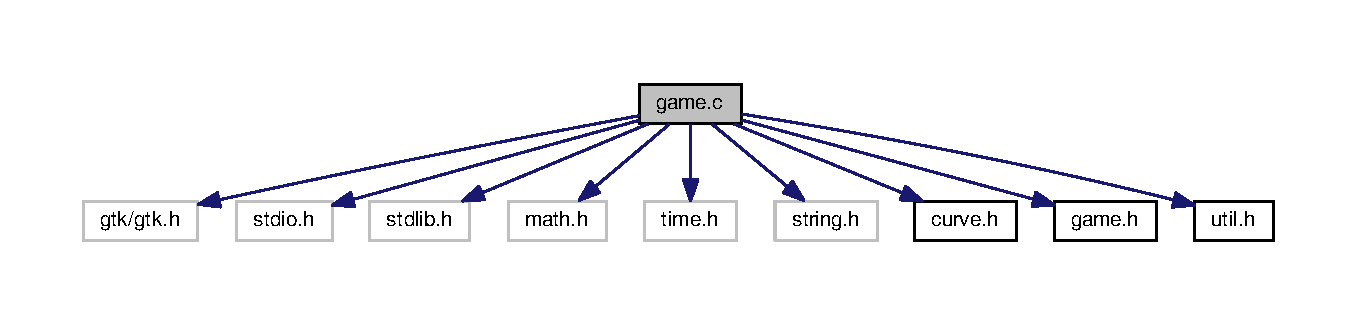
\includegraphics[width=350pt]{game_8c__incl}
\end{center}
\end{figure}
\subsection*{Functions}
\begin{DoxyCompactItemize}
\item 
void \hyperlink{game_8c_a1379e442012bd2db4e0a7c43ba12a140}{sample\+\_\+curve\+\_\+to\+\_\+track} (\hyperlink{struct_curve}{Curve} $\ast$curve, \hyperlink{struct_track}{Track} $\ast$track, double theta)
\begin{DoxyCompactList}\small\item\em Fonction de conversion d\textquotesingle{}une curve en une track. \end{DoxyCompactList}\item 
void {\bfseries shoot\+\_\+ammo} (\hyperlink{struct_game}{Game} $\ast$game)\hypertarget{game_8c_a7a28065cd246ecccf78c7b940b4b6651}{}\label{game_8c_a7a28065cd246ecccf78c7b940b4b6651}

\item 
int \hyperlink{game_8c_a32dbc2ae6d9dd615b664c16ef04bf376}{is\+\_\+color\+\_\+on\+\_\+track} (\hyperlink{struct_track}{Track} $\ast$track, int color)
\begin{DoxyCompactList}\small\item\em Fonction pour chercher si une couleur est dans la track. \end{DoxyCompactList}\item 
void \hyperlink{game_8c_aaf45176a520f6cfd9d8a52c140802a5d}{prepare\+\_\+ammo} (\hyperlink{struct_game}{Game} $\ast$game)
\begin{DoxyCompactList}\small\item\em Fonction pour préparer les balles du canon après un tir. \end{DoxyCompactList}\item 
void \hyperlink{game_8c_a561e64089b963fcb06eff3c654bc8585}{swap\+\_\+ammo} (\hyperlink{struct_game}{Game} $\ast$game)
\begin{DoxyCompactList}\small\item\em Fonction pour echanger les balles du canon. \end{DoxyCompactList}\item 
void \hyperlink{game_8c_a321533d866fea72c822dabdeb0ccc094}{game\+\_\+pause} (\hyperlink{struct_game}{Game} $\ast$game)
\begin{DoxyCompactList}\small\item\em Fonction pour mettre en pause le jeu si il ne l\textquotesingle{}est pas sinon le remet en mode playing. \end{DoxyCompactList}\item 
int \hyperlink{game_8c_aa5b5a4c5c922fe5aa18ef28ac693db5a}{calcule\+\_\+score\+\_\+with\+\_\+marble\+\_\+group\+\_\+size} (\hyperlink{struct_game}{Game} $\ast$game, \hyperlink{struct_track}{Track} $\ast$track, int marble\+\_\+id\+\_\+start, int score, int combo)
\begin{DoxyCompactList}\small\item\em Fonction pour calculer le score obtenu après un tir. \end{DoxyCompactList}\item 
void \hyperlink{game_8c_a6a5803be3dedb50a82b3d625ac90ea3e}{check\+\_\+bonus} (\hyperlink{struct_game}{Game} $\ast$game, \hyperlink{struct_track}{Track} $\ast$track, int marble)
\begin{DoxyCompactList}\small\item\em Fonction pour vérifier si il y a un bonus. \end{DoxyCompactList}\item 
void \hyperlink{game_8c_a171ea500d411c5194613976786047d70}{check\+\_\+bonus\+\_\+end} (\hyperlink{struct_game}{Game} $\ast$game)
\begin{DoxyCompactList}\small\item\em Fonction pour vérifier un bonus est terminé \end{DoxyCompactList}\item 
void \hyperlink{game_8c_a4476eab4b74a53b36cdf7d7096c62060}{move\+\_\+shots\+\_\+one\+\_\+step} (\hyperlink{struct_game}{Game} $\ast$game)
\begin{DoxyCompactList}\small\item\em Fonction pour avancer le shot. \end{DoxyCompactList}\item 
void \hyperlink{game_8c_a401c25af3ee1e41a353329513c7fb679}{suppress\+\_\+far\+\_\+shots} (\hyperlink{struct_game}{Game} $\ast$game, int screen\+\_\+width, int screen\+\_\+height)
\begin{DoxyCompactList}\small\item\em Fonction de suppression des tirs lointains. \end{DoxyCompactList}\item 
void \hyperlink{game_8c_a590c19b4c7fbc37e84976b4d3773e0b7}{do\+\_\+vector\+\_\+product} (double xu, double yu, double zu, double xv, double yv, double zv, double $\ast$x, double $\ast$y, double $\ast$z)
\item 
int \hyperlink{game_8c_a868a0d63645e599dd01aee704da37251}{test\+\_\+collision} (\hyperlink{struct_game}{Game} $\ast$game, int $\ast$shot\+\_\+num, int $\ast$marble\+\_\+num, int track\+\_\+num)
\begin{DoxyCompactList}\small\item\em fonctione pour tester si il y a une colision entre un shot et une bille du train \end{DoxyCompactList}\item 
void \hyperlink{game_8c_a903a06d0784febcd3fdcf811cc71a28f}{process\+\_\+shots\+\_\+collisions} (\hyperlink{struct_game}{Game} $\ast$game)
\begin{DoxyCompactList}\small\item\em insertion de la bille si il y a eu colision \end{DoxyCompactList}\item 
void \hyperlink{game_8c_a82438caca3314471bef10e102441af12}{move\+\_\+trains\+\_\+one\+\_\+step} (\hyperlink{struct_game}{Game} $\ast$game)
\begin{DoxyCompactList}\small\item\em Fonction pour faire avancer le train. \end{DoxyCompactList}\item 
void \hyperlink{game_8c_aa5da90408ff8ede3b09fa6a0a376c709}{check\+\_\+end\+\_\+of\+\_\+game} (\hyperlink{struct_game}{Game} $\ast$game)
\begin{DoxyCompactList}\small\item\em Fonction pour vérifier si la partie est terminé \end{DoxyCompactList}\item 
void \hyperlink{game_8c_a5b35e1416156b7ae084045350ba89ab9}{progress\+\_\+game\+\_\+next\+\_\+step} (\hyperlink{struct_game}{Game} $\ast$game, int screen\+\_\+width, int screen\+\_\+height)
\begin{DoxyCompactList}\small\item\em Fonction d\textquotesingle{}étape du jeu (boucle principale) \end{DoxyCompactList}\item 
void \hyperlink{game_8c_adad209d500c35da1b3d4985e7a09bec4}{update\+\_\+canon\+\_\+angle} (\hyperlink{struct_game}{Game} $\ast$game, double sx, double sy)
\begin{DoxyCompactList}\small\item\em Fonction pour mettre à jour l\textquotesingle{}angle du canon. \end{DoxyCompactList}\item 
void \hyperlink{game_8c_a5c95bbb5adb20ea2cbf4ed0bc1c9025f}{load\+\_\+cannon\+\_\+image} (\hyperlink{struct_game}{Game} $\ast$game)
\begin{DoxyCompactList}\small\item\em Fonction pour charger l\textquotesingle{}image du canon. \end{DoxyCompactList}\item 
void \hyperlink{game_8c_a737ca8731777960973c03c78e1d777d7}{update\+\_\+x\+\_\+and\+\_\+y\+\_\+canon} (\hyperlink{struct_game}{Game} $\ast$game, int height, int width)
\begin{DoxyCompactList}\small\item\em Fonction de mise à jour de la postion du canon par rapport à l\textquotesingle{}écran pour le centrer. \end{DoxyCompactList}\item 
void \hyperlink{game_8c_aa832339540d987f842a7d505da20803c}{init\+\_\+canon} (\hyperlink{struct_game}{Game} $\ast$game, int height, int width)
\begin{DoxyCompactList}\small\item\em Fonction pour l\textquotesingle{}initialisation du canon. \end{DoxyCompactList}\item 
void \hyperlink{game_8c_afd103f2ed5a4accadde77c8f8fbe489b}{init\+\_\+ammo} (\hyperlink{struct_game}{Game} $\ast$game)
\begin{DoxyCompactList}\small\item\em Fonction pour l\textquotesingle{}initialisation des munitions du canon. \end{DoxyCompactList}\item 
void \hyperlink{game_8c_a76bc3a19eb94631d39401b92e638d529}{init\+\_\+shots} (\hyperlink{struct_game}{Game} $\ast$game)
\begin{DoxyCompactList}\small\item\em Fonction pour l\textquotesingle{}initialisation des shots. \end{DoxyCompactList}\item 
int \hyperlink{game_8c_aec4660f64205ee890c1c609f7883cd16}{init\+\_\+marble\+\_\+bonus} ()
\begin{DoxyCompactList}\small\item\em Fonction pour la génération du bonus aléatoirement. \end{DoxyCompactList}\item 
void \hyperlink{game_8c_a090892ad996749a780a8f8c7670a853d}{create\+\_\+marbles} (\hyperlink{struct_track}{Track} $\ast$track, int current\+\_\+level)
\begin{DoxyCompactList}\small\item\em Fonction pour créer les billes. \end{DoxyCompactList}\item 
void \hyperlink{game_8c_af1c8645a911806b783052f96c2f9f96d}{init\+\_\+track} (\hyperlink{struct_game}{Game} $\ast$game)
\begin{DoxyCompactList}\small\item\em Fonction pour l\textquotesingle{}initialisation de la track. \end{DoxyCompactList}\item 
void \hyperlink{game_8c_a1aa823f431873e33d5b7095aaf8199f8}{init\+\_\+game} (\hyperlink{struct_game}{Game} $\ast$game, int height, int width)
\begin{DoxyCompactList}\small\item\em Fonction pour l\textquotesingle{}initialisation du jeu. \end{DoxyCompactList}\item 
void \hyperlink{game_8c_a96baae852b652337739b9cf463ec9a5f}{reset\+\_\+game} (\hyperlink{struct_game}{Game} $\ast$game, int height, int width)
\begin{DoxyCompactList}\small\item\em Fonction de réinitialisation du jeu. \end{DoxyCompactList}\item 
void \hyperlink{game_8c_a971b5b9e0391b68e00546b19fe07bafb}{restart\+\_\+game} (\hyperlink{struct_game}{Game} $\ast$game, int height, int width)
\begin{DoxyCompactList}\small\item\em Fonction pour recommencer un level. \end{DoxyCompactList}\item 
void \hyperlink{game_8c_a055ce2874a0fbed77092e4ba81c59ddf}{change\+\_\+level} (\hyperlink{struct_game}{Game} $\ast$game, int height, int width)
\begin{DoxyCompactList}\small\item\em Fonction pour changer de level. \end{DoxyCompactList}\item 
void \hyperlink{game_8c_ab5fc2f364ae1501956a2958de19cbe97}{time\+\_\+stop} (\hyperlink{struct_game}{Game} $\ast$game)
\begin{DoxyCompactList}\small\item\em Fonction pour arrêter le temps ( le train) \end{DoxyCompactList}\item 
void \hyperlink{game_8c_ad88ea8e0d2afe0c3987e18e586274c1b}{speed\+\_\+change} (\hyperlink{struct_game}{Game} $\ast$game, int bonus)
\begin{DoxyCompactList}\small\item\em Fonction pour changer la vitesse du train, accélérer ou bien ralentir. \end{DoxyCompactList}\end{DoxyCompactItemize}


\subsection{Detailed Description}
Fonctions et objets principaux du jeu. 

\begin{DoxyAuthor}{Author}
Gaëtan Perrot 
\end{DoxyAuthor}
\begin{DoxyVersion}{Version}
0.\+1 
\end{DoxyVersion}
\begin{DoxyDate}{Date}
23 avril 2017
\end{DoxyDate}
Fonctions et objets principaux du jeu 

\subsection{Function Documentation}
\index{game.\+c@{game.\+c}!calcule\+\_\+score\+\_\+with\+\_\+marble\+\_\+group\+\_\+size@{calcule\+\_\+score\+\_\+with\+\_\+marble\+\_\+group\+\_\+size}}
\index{calcule\+\_\+score\+\_\+with\+\_\+marble\+\_\+group\+\_\+size@{calcule\+\_\+score\+\_\+with\+\_\+marble\+\_\+group\+\_\+size}!game.\+c@{game.\+c}}
\subsubsection[{\texorpdfstring{calcule\+\_\+score\+\_\+with\+\_\+marble\+\_\+group\+\_\+size(\+Game $\ast$game, Track $\ast$track, int marble\+\_\+id\+\_\+start, int score, int combo)}{calcule_score_with_marble_group_size(Game *game, Track *track, int marble_id_start, int score, int combo)}}]{\setlength{\rightskip}{0pt plus 5cm}int calcule\+\_\+score\+\_\+with\+\_\+marble\+\_\+group\+\_\+size (
\begin{DoxyParamCaption}
\item[{{\bf Game} $\ast$}]{game, }
\item[{{\bf Track} $\ast$}]{track, }
\item[{int}]{marble\+\_\+id\+\_\+start, }
\item[{int}]{score, }
\item[{int}]{bonus}
\end{DoxyParamCaption}
)}\hypertarget{game_8c_aa5b5a4c5c922fe5aa18ef28ac693db5a}{}\label{game_8c_aa5b5a4c5c922fe5aa18ef28ac693db5a}


Fonction pour calculer le score obtenu après un tir. 


\begin{DoxyParams}{Parameters}
{\em self} & Objet \hyperlink{struct_game}{Game} $\ast$ game,\hyperlink{struct_track}{Track} $\ast$ track, int marble\+\_\+id\+\_\+start,int score,int bonus \\
\hline
\end{DoxyParams}
\begin{DoxyReturn}{Returns}
int 
\end{DoxyReturn}
\index{game.\+c@{game.\+c}!change\+\_\+level@{change\+\_\+level}}
\index{change\+\_\+level@{change\+\_\+level}!game.\+c@{game.\+c}}
\subsubsection[{\texorpdfstring{change\+\_\+level(\+Game $\ast$game, int height, int width)}{change_level(Game *game, int height, int width)}}]{\setlength{\rightskip}{0pt plus 5cm}void change\+\_\+level (
\begin{DoxyParamCaption}
\item[{{\bf Game} $\ast$}]{game, }
\item[{int}]{height, }
\item[{int}]{width}
\end{DoxyParamCaption}
)}\hypertarget{game_8c_a055ce2874a0fbed77092e4ba81c59ddf}{}\label{game_8c_a055ce2874a0fbed77092e4ba81c59ddf}


Fonction pour changer de level. 


\begin{DoxyParams}{Parameters}
{\em self} & \hyperlink{struct_game}{Game} $\ast$ game, int height, int width \\
\hline
\end{DoxyParams}
\begin{DoxyReturn}{Returns}
void 
\end{DoxyReturn}
\index{game.\+c@{game.\+c}!check\+\_\+bonus@{check\+\_\+bonus}}
\index{check\+\_\+bonus@{check\+\_\+bonus}!game.\+c@{game.\+c}}
\subsubsection[{\texorpdfstring{check\+\_\+bonus(\+Game $\ast$game, Track $\ast$track, int marble)}{check_bonus(Game *game, Track *track, int marble)}}]{\setlength{\rightskip}{0pt plus 5cm}void check\+\_\+bonus (
\begin{DoxyParamCaption}
\item[{{\bf Game} $\ast$}]{game, }
\item[{{\bf Track} $\ast$}]{track, }
\item[{int}]{marble}
\end{DoxyParamCaption}
)}\hypertarget{game_8c_a6a5803be3dedb50a82b3d625ac90ea3e}{}\label{game_8c_a6a5803be3dedb50a82b3d625ac90ea3e}


Fonction pour vérifier si il y a un bonus. 


\begin{DoxyParams}{Parameters}
{\em self} & Objet \hyperlink{struct_game}{Game} $\ast$ game,\hyperlink{struct_track}{Track} $\ast$ track,int marble \\
\hline
\end{DoxyParams}
\begin{DoxyReturn}{Returns}
void 
\end{DoxyReturn}
\index{game.\+c@{game.\+c}!check\+\_\+bonus\+\_\+end@{check\+\_\+bonus\+\_\+end}}
\index{check\+\_\+bonus\+\_\+end@{check\+\_\+bonus\+\_\+end}!game.\+c@{game.\+c}}
\subsubsection[{\texorpdfstring{check\+\_\+bonus\+\_\+end(\+Game $\ast$game)}{check_bonus_end(Game *game)}}]{\setlength{\rightskip}{0pt plus 5cm}void check\+\_\+bonus\+\_\+end (
\begin{DoxyParamCaption}
\item[{{\bf Game} $\ast$}]{game}
\end{DoxyParamCaption}
)}\hypertarget{game_8c_a171ea500d411c5194613976786047d70}{}\label{game_8c_a171ea500d411c5194613976786047d70}


Fonction pour vérifier un bonus est terminé 


\begin{DoxyParams}{Parameters}
{\em self} & Objet \hyperlink{struct_game}{Game} \\
\hline
\end{DoxyParams}
\begin{DoxyReturn}{Returns}
void 
\end{DoxyReturn}
\index{game.\+c@{game.\+c}!check\+\_\+end\+\_\+of\+\_\+game@{check\+\_\+end\+\_\+of\+\_\+game}}
\index{check\+\_\+end\+\_\+of\+\_\+game@{check\+\_\+end\+\_\+of\+\_\+game}!game.\+c@{game.\+c}}
\subsubsection[{\texorpdfstring{check\+\_\+end\+\_\+of\+\_\+game(\+Game $\ast$game)}{check_end_of_game(Game *game)}}]{\setlength{\rightskip}{0pt plus 5cm}void check\+\_\+end\+\_\+of\+\_\+game (
\begin{DoxyParamCaption}
\item[{{\bf Game} $\ast$}]{game}
\end{DoxyParamCaption}
)}\hypertarget{game_8c_aa5da90408ff8ede3b09fa6a0a376c709}{}\label{game_8c_aa5da90408ff8ede3b09fa6a0a376c709}


Fonction pour vérifier si la partie est terminé 


\begin{DoxyParams}{Parameters}
{\em self} & \hyperlink{struct_game}{Game} $\ast$ game \\
\hline
\end{DoxyParams}
\begin{DoxyReturn}{Returns}
void 
\end{DoxyReturn}
\index{game.\+c@{game.\+c}!create\+\_\+marbles@{create\+\_\+marbles}}
\index{create\+\_\+marbles@{create\+\_\+marbles}!game.\+c@{game.\+c}}
\subsubsection[{\texorpdfstring{create\+\_\+marbles(\+Track $\ast$track, int current\+\_\+level)}{create_marbles(Track *track, int current_level)}}]{\setlength{\rightskip}{0pt plus 5cm}void create\+\_\+marbles (
\begin{DoxyParamCaption}
\item[{{\bf Track} $\ast$}]{track, }
\item[{int}]{current\+\_\+level}
\end{DoxyParamCaption}
)}\hypertarget{game_8c_a090892ad996749a780a8f8c7670a853d}{}\label{game_8c_a090892ad996749a780a8f8c7670a853d}


Fonction pour créer les billes. 


\begin{DoxyParams}{Parameters}
{\em self} & \hyperlink{struct_track}{Track} $\ast$ track,int current\+\_\+level \\
\hline
\end{DoxyParams}
\begin{DoxyReturn}{Returns}
void 
\end{DoxyReturn}
\index{game.\+c@{game.\+c}!do\+\_\+vector\+\_\+product@{do\+\_\+vector\+\_\+product}}
\index{do\+\_\+vector\+\_\+product@{do\+\_\+vector\+\_\+product}!game.\+c@{game.\+c}}
\subsubsection[{\texorpdfstring{do\+\_\+vector\+\_\+product(double xu, double yu, double zu, double xv, double yv, double zv, double $\ast$x, double $\ast$y, double $\ast$z)}{do_vector_product(double xu, double yu, double zu, double xv, double yv, double zv, double *x, double *y, double *z)}}]{\setlength{\rightskip}{0pt plus 5cm}void do\+\_\+vector\+\_\+product (
\begin{DoxyParamCaption}
\item[{double}]{xu, }
\item[{double}]{yu, }
\item[{double}]{zu, }
\item[{double}]{xv, }
\item[{double}]{yv, }
\item[{double}]{zv, }
\item[{double $\ast$}]{x, }
\item[{double $\ast$}]{y, }
\item[{double $\ast$}]{z}
\end{DoxyParamCaption}
)}\hypertarget{game_8c_a590c19b4c7fbc37e84976b4d3773e0b7}{}\label{game_8c_a590c19b4c7fbc37e84976b4d3773e0b7}

\begin{DoxyParams}{Parameters}
{\em self} & double xu,double yu,double zu,double xv,double yv,double zv, double $\ast$x, double $\ast$y,double $\ast$z) \\
\hline
\end{DoxyParams}
\begin{DoxyReturn}{Returns}
void 
\end{DoxyReturn}
\index{game.\+c@{game.\+c}!game\+\_\+pause@{game\+\_\+pause}}
\index{game\+\_\+pause@{game\+\_\+pause}!game.\+c@{game.\+c}}
\subsubsection[{\texorpdfstring{game\+\_\+pause(\+Game $\ast$game)}{game_pause(Game *game)}}]{\setlength{\rightskip}{0pt plus 5cm}void game\+\_\+pause (
\begin{DoxyParamCaption}
\item[{{\bf Game} $\ast$}]{game}
\end{DoxyParamCaption}
)}\hypertarget{game_8c_a321533d866fea72c822dabdeb0ccc094}{}\label{game_8c_a321533d866fea72c822dabdeb0ccc094}


Fonction pour mettre en pause le jeu si il ne l\textquotesingle{}est pas sinon le remet en mode playing. 


\begin{DoxyParams}{Parameters}
{\em self} & Objet \hyperlink{struct_game}{Game} \\
\hline
\end{DoxyParams}
\begin{DoxyReturn}{Returns}
void 
\end{DoxyReturn}
\index{game.\+c@{game.\+c}!init\+\_\+ammo@{init\+\_\+ammo}}
\index{init\+\_\+ammo@{init\+\_\+ammo}!game.\+c@{game.\+c}}
\subsubsection[{\texorpdfstring{init\+\_\+ammo(\+Game $\ast$game)}{init_ammo(Game *game)}}]{\setlength{\rightskip}{0pt plus 5cm}void init\+\_\+ammo (
\begin{DoxyParamCaption}
\item[{{\bf Game} $\ast$}]{game}
\end{DoxyParamCaption}
)}\hypertarget{game_8c_afd103f2ed5a4accadde77c8f8fbe489b}{}\label{game_8c_afd103f2ed5a4accadde77c8f8fbe489b}


Fonction pour l\textquotesingle{}initialisation des munitions du canon. 


\begin{DoxyParams}{Parameters}
{\em self} & \hyperlink{struct_game}{Game} $\ast$ game \\
\hline
\end{DoxyParams}
\begin{DoxyReturn}{Returns}
void 
\end{DoxyReturn}
\index{game.\+c@{game.\+c}!init\+\_\+canon@{init\+\_\+canon}}
\index{init\+\_\+canon@{init\+\_\+canon}!game.\+c@{game.\+c}}
\subsubsection[{\texorpdfstring{init\+\_\+canon(\+Game $\ast$game, int height, int width)}{init_canon(Game *game, int height, int width)}}]{\setlength{\rightskip}{0pt plus 5cm}void init\+\_\+canon (
\begin{DoxyParamCaption}
\item[{{\bf Game} $\ast$}]{game, }
\item[{int}]{height, }
\item[{int}]{width}
\end{DoxyParamCaption}
)}\hypertarget{game_8c_aa832339540d987f842a7d505da20803c}{}\label{game_8c_aa832339540d987f842a7d505da20803c}


Fonction pour l\textquotesingle{}initialisation du canon. 


\begin{DoxyParams}{Parameters}
{\em self} & \hyperlink{struct_game}{Game} $\ast$ game,int height, int width \\
\hline
\end{DoxyParams}
\begin{DoxyReturn}{Returns}
void 
\end{DoxyReturn}
\index{game.\+c@{game.\+c}!init\+\_\+game@{init\+\_\+game}}
\index{init\+\_\+game@{init\+\_\+game}!game.\+c@{game.\+c}}
\subsubsection[{\texorpdfstring{init\+\_\+game(\+Game $\ast$game, int height, int width)}{init_game(Game *game, int height, int width)}}]{\setlength{\rightskip}{0pt plus 5cm}void init\+\_\+game (
\begin{DoxyParamCaption}
\item[{{\bf Game} $\ast$}]{game, }
\item[{int}]{height, }
\item[{int}]{width}
\end{DoxyParamCaption}
)}\hypertarget{game_8c_a1aa823f431873e33d5b7095aaf8199f8}{}\label{game_8c_a1aa823f431873e33d5b7095aaf8199f8}


Fonction pour l\textquotesingle{}initialisation du jeu. 


\begin{DoxyParams}{Parameters}
{\em self} & \hyperlink{struct_game}{Game} $\ast$ game, int height, int width \\
\hline
\end{DoxyParams}
\begin{DoxyReturn}{Returns}
void 
\end{DoxyReturn}
\index{game.\+c@{game.\+c}!init\+\_\+marble\+\_\+bonus@{init\+\_\+marble\+\_\+bonus}}
\index{init\+\_\+marble\+\_\+bonus@{init\+\_\+marble\+\_\+bonus}!game.\+c@{game.\+c}}
\subsubsection[{\texorpdfstring{init\+\_\+marble\+\_\+bonus()}{init_marble_bonus()}}]{\setlength{\rightskip}{0pt plus 5cm}int init\+\_\+marble\+\_\+bonus (
\begin{DoxyParamCaption}
{}
\end{DoxyParamCaption}
)}\hypertarget{game_8c_aec4660f64205ee890c1c609f7883cd16}{}\label{game_8c_aec4660f64205ee890c1c609f7883cd16}


Fonction pour la génération du bonus aléatoirement. 


\begin{DoxyParams}{Parameters}
{\em self} & \\
\hline
\end{DoxyParams}
\begin{DoxyReturn}{Returns}
int le bonus généré aléatoirement 
\end{DoxyReturn}
\index{game.\+c@{game.\+c}!init\+\_\+shots@{init\+\_\+shots}}
\index{init\+\_\+shots@{init\+\_\+shots}!game.\+c@{game.\+c}}
\subsubsection[{\texorpdfstring{init\+\_\+shots(\+Game $\ast$game)}{init_shots(Game *game)}}]{\setlength{\rightskip}{0pt plus 5cm}void init\+\_\+shots (
\begin{DoxyParamCaption}
\item[{{\bf Game} $\ast$}]{game}
\end{DoxyParamCaption}
)}\hypertarget{game_8c_a76bc3a19eb94631d39401b92e638d529}{}\label{game_8c_a76bc3a19eb94631d39401b92e638d529}


Fonction pour l\textquotesingle{}initialisation des shots. 


\begin{DoxyParams}{Parameters}
{\em self} & \hyperlink{struct_game}{Game} $\ast$ game \\
\hline
\end{DoxyParams}
\begin{DoxyReturn}{Returns}
void 
\end{DoxyReturn}
\index{game.\+c@{game.\+c}!init\+\_\+track@{init\+\_\+track}}
\index{init\+\_\+track@{init\+\_\+track}!game.\+c@{game.\+c}}
\subsubsection[{\texorpdfstring{init\+\_\+track(\+Game $\ast$game)}{init_track(Game *game)}}]{\setlength{\rightskip}{0pt plus 5cm}void init\+\_\+track (
\begin{DoxyParamCaption}
\item[{{\bf Game} $\ast$}]{game}
\end{DoxyParamCaption}
)}\hypertarget{game_8c_af1c8645a911806b783052f96c2f9f96d}{}\label{game_8c_af1c8645a911806b783052f96c2f9f96d}


Fonction pour l\textquotesingle{}initialisation de la track. 


\begin{DoxyParams}{Parameters}
{\em self} & \hyperlink{struct_game}{Game} $\ast$ game \\
\hline
\end{DoxyParams}
\begin{DoxyReturn}{Returns}
void 
\end{DoxyReturn}
\index{game.\+c@{game.\+c}!is\+\_\+color\+\_\+on\+\_\+track@{is\+\_\+color\+\_\+on\+\_\+track}}
\index{is\+\_\+color\+\_\+on\+\_\+track@{is\+\_\+color\+\_\+on\+\_\+track}!game.\+c@{game.\+c}}
\subsubsection[{\texorpdfstring{is\+\_\+color\+\_\+on\+\_\+track(\+Track $\ast$track, int color)}{is_color_on_track(Track *track, int color)}}]{\setlength{\rightskip}{0pt plus 5cm}int is\+\_\+color\+\_\+on\+\_\+track (
\begin{DoxyParamCaption}
\item[{{\bf Track} $\ast$}]{track, }
\item[{int}]{color}
\end{DoxyParamCaption}
)}\hypertarget{game_8c_a32dbc2ae6d9dd615b664c16ef04bf376}{}\label{game_8c_a32dbc2ae6d9dd615b664c16ef04bf376}


Fonction pour chercher si une couleur est dans la track. 


\begin{DoxyParams}{Parameters}
{\em self} & Objet \hyperlink{struct_track}{Track} $\ast$ track, int color \\
\hline
\end{DoxyParams}
\begin{DoxyReturn}{Returns}
retourne 1 si la couleur est déjà dans la track et 0 si elle ne l\textquotesingle{}ait pas 
\end{DoxyReturn}
\index{game.\+c@{game.\+c}!load\+\_\+cannon\+\_\+image@{load\+\_\+cannon\+\_\+image}}
\index{load\+\_\+cannon\+\_\+image@{load\+\_\+cannon\+\_\+image}!game.\+c@{game.\+c}}
\subsubsection[{\texorpdfstring{load\+\_\+cannon\+\_\+image(\+Game $\ast$game)}{load_cannon_image(Game *game)}}]{\setlength{\rightskip}{0pt plus 5cm}void load\+\_\+cannon\+\_\+image (
\begin{DoxyParamCaption}
\item[{{\bf Game} $\ast$}]{game}
\end{DoxyParamCaption}
)}\hypertarget{game_8c_a5c95bbb5adb20ea2cbf4ed0bc1c9025f}{}\label{game_8c_a5c95bbb5adb20ea2cbf4ed0bc1c9025f}


Fonction pour charger l\textquotesingle{}image du canon. 


\begin{DoxyParams}{Parameters}
{\em self} & \hyperlink{struct_game}{Game} $\ast$ game \\
\hline
\end{DoxyParams}
\begin{DoxyReturn}{Returns}
void 
\end{DoxyReturn}
\index{game.\+c@{game.\+c}!move\+\_\+shots\+\_\+one\+\_\+step@{move\+\_\+shots\+\_\+one\+\_\+step}}
\index{move\+\_\+shots\+\_\+one\+\_\+step@{move\+\_\+shots\+\_\+one\+\_\+step}!game.\+c@{game.\+c}}
\subsubsection[{\texorpdfstring{move\+\_\+shots\+\_\+one\+\_\+step(\+Game $\ast$game)}{move_shots_one_step(Game *game)}}]{\setlength{\rightskip}{0pt plus 5cm}void move\+\_\+shots\+\_\+one\+\_\+step (
\begin{DoxyParamCaption}
\item[{{\bf Game} $\ast$}]{game}
\end{DoxyParamCaption}
)}\hypertarget{game_8c_a4476eab4b74a53b36cdf7d7096c62060}{}\label{game_8c_a4476eab4b74a53b36cdf7d7096c62060}


Fonction pour avancer le shot. 


\begin{DoxyParams}{Parameters}
{\em self} & Objet \hyperlink{struct_game}{Game} \\
\hline
\end{DoxyParams}
\begin{DoxyReturn}{Returns}
void 
\end{DoxyReturn}
\index{game.\+c@{game.\+c}!move\+\_\+trains\+\_\+one\+\_\+step@{move\+\_\+trains\+\_\+one\+\_\+step}}
\index{move\+\_\+trains\+\_\+one\+\_\+step@{move\+\_\+trains\+\_\+one\+\_\+step}!game.\+c@{game.\+c}}
\subsubsection[{\texorpdfstring{move\+\_\+trains\+\_\+one\+\_\+step(\+Game $\ast$game)}{move_trains_one_step(Game *game)}}]{\setlength{\rightskip}{0pt plus 5cm}void move\+\_\+trains\+\_\+one\+\_\+step (
\begin{DoxyParamCaption}
\item[{{\bf Game} $\ast$}]{game}
\end{DoxyParamCaption}
)}\hypertarget{game_8c_a82438caca3314471bef10e102441af12}{}\label{game_8c_a82438caca3314471bef10e102441af12}


Fonction pour faire avancer le train. 


\begin{DoxyParams}{Parameters}
{\em self} & \hyperlink{struct_game}{Game} $\ast$ game \\
\hline
\end{DoxyParams}
\begin{DoxyReturn}{Returns}
void 
\end{DoxyReturn}
\index{game.\+c@{game.\+c}!prepare\+\_\+ammo@{prepare\+\_\+ammo}}
\index{prepare\+\_\+ammo@{prepare\+\_\+ammo}!game.\+c@{game.\+c}}
\subsubsection[{\texorpdfstring{prepare\+\_\+ammo(\+Game $\ast$game)}{prepare_ammo(Game *game)}}]{\setlength{\rightskip}{0pt plus 5cm}void prepare\+\_\+ammo (
\begin{DoxyParamCaption}
\item[{{\bf Game} $\ast$}]{game}
\end{DoxyParamCaption}
)}\hypertarget{game_8c_aaf45176a520f6cfd9d8a52c140802a5d}{}\label{game_8c_aaf45176a520f6cfd9d8a52c140802a5d}


Fonction pour préparer les balles du canon après un tir. 


\begin{DoxyParams}{Parameters}
{\em self} & Objet \hyperlink{struct_game}{Game} \\
\hline
\end{DoxyParams}
\begin{DoxyReturn}{Returns}
void 
\end{DoxyReturn}
\index{game.\+c@{game.\+c}!process\+\_\+shots\+\_\+collisions@{process\+\_\+shots\+\_\+collisions}}
\index{process\+\_\+shots\+\_\+collisions@{process\+\_\+shots\+\_\+collisions}!game.\+c@{game.\+c}}
\subsubsection[{\texorpdfstring{process\+\_\+shots\+\_\+collisions(\+Game $\ast$game)}{process_shots_collisions(Game *game)}}]{\setlength{\rightskip}{0pt plus 5cm}void process\+\_\+shots\+\_\+collisions (
\begin{DoxyParamCaption}
\item[{{\bf Game} $\ast$}]{game}
\end{DoxyParamCaption}
)}\hypertarget{game_8c_a903a06d0784febcd3fdcf811cc71a28f}{}\label{game_8c_a903a06d0784febcd3fdcf811cc71a28f}


insertion de la bille si il y a eu colision 


\begin{DoxyParams}{Parameters}
{\em self} & \hyperlink{struct_game}{Game} $\ast$ game \\
\hline
\end{DoxyParams}
\begin{DoxyReturn}{Returns}
void 
\end{DoxyReturn}
\index{game.\+c@{game.\+c}!progress\+\_\+game\+\_\+next\+\_\+step@{progress\+\_\+game\+\_\+next\+\_\+step}}
\index{progress\+\_\+game\+\_\+next\+\_\+step@{progress\+\_\+game\+\_\+next\+\_\+step}!game.\+c@{game.\+c}}
\subsubsection[{\texorpdfstring{progress\+\_\+game\+\_\+next\+\_\+step(\+Game $\ast$game, int screen\+\_\+width, int screen\+\_\+height)}{progress_game_next_step(Game *game, int screen_width, int screen_height)}}]{\setlength{\rightskip}{0pt plus 5cm}void progress\+\_\+game\+\_\+next\+\_\+step (
\begin{DoxyParamCaption}
\item[{{\bf Game} $\ast$}]{game, }
\item[{int}]{screen\+\_\+width, }
\item[{int}]{screen\+\_\+height}
\end{DoxyParamCaption}
)}\hypertarget{game_8c_a5b35e1416156b7ae084045350ba89ab9}{}\label{game_8c_a5b35e1416156b7ae084045350ba89ab9}


Fonction d\textquotesingle{}étape du jeu (boucle principale) 


\begin{DoxyParams}{Parameters}
{\em self} & \hyperlink{struct_game}{Game} $\ast$ game,int screen\+\_\+width, int screen\+\_\+height \\
\hline
\end{DoxyParams}
\begin{DoxyReturn}{Returns}
void 
\end{DoxyReturn}
\index{game.\+c@{game.\+c}!reset\+\_\+game@{reset\+\_\+game}}
\index{reset\+\_\+game@{reset\+\_\+game}!game.\+c@{game.\+c}}
\subsubsection[{\texorpdfstring{reset\+\_\+game(\+Game $\ast$game, int height, int width)}{reset_game(Game *game, int height, int width)}}]{\setlength{\rightskip}{0pt plus 5cm}void reset\+\_\+game (
\begin{DoxyParamCaption}
\item[{{\bf Game} $\ast$}]{game, }
\item[{int}]{height, }
\item[{int}]{width}
\end{DoxyParamCaption}
)}\hypertarget{game_8c_a96baae852b652337739b9cf463ec9a5f}{}\label{game_8c_a96baae852b652337739b9cf463ec9a5f}


Fonction de réinitialisation du jeu. 


\begin{DoxyParams}{Parameters}
{\em self} & \hyperlink{struct_game}{Game} $\ast$ game, int height, int width \\
\hline
\end{DoxyParams}
\begin{DoxyReturn}{Returns}
void 
\end{DoxyReturn}
\index{game.\+c@{game.\+c}!restart\+\_\+game@{restart\+\_\+game}}
\index{restart\+\_\+game@{restart\+\_\+game}!game.\+c@{game.\+c}}
\subsubsection[{\texorpdfstring{restart\+\_\+game(\+Game $\ast$game, int height, int width)}{restart_game(Game *game, int height, int width)}}]{\setlength{\rightskip}{0pt plus 5cm}void restart\+\_\+game (
\begin{DoxyParamCaption}
\item[{{\bf Game} $\ast$}]{game, }
\item[{int}]{height, }
\item[{int}]{width}
\end{DoxyParamCaption}
)}\hypertarget{game_8c_a971b5b9e0391b68e00546b19fe07bafb}{}\label{game_8c_a971b5b9e0391b68e00546b19fe07bafb}


Fonction pour recommencer un level. 


\begin{DoxyParams}{Parameters}
{\em self} & \hyperlink{struct_game}{Game} $\ast$ game, int height, int width \\
\hline
\end{DoxyParams}
\begin{DoxyReturn}{Returns}
void 
\end{DoxyReturn}
\index{game.\+c@{game.\+c}!sample\+\_\+curve\+\_\+to\+\_\+track@{sample\+\_\+curve\+\_\+to\+\_\+track}}
\index{sample\+\_\+curve\+\_\+to\+\_\+track@{sample\+\_\+curve\+\_\+to\+\_\+track}!game.\+c@{game.\+c}}
\subsubsection[{\texorpdfstring{sample\+\_\+curve\+\_\+to\+\_\+track(\+Curve $\ast$curve, Track $\ast$track, double theta)}{sample_curve_to_track(Curve *curve, Track *track, double theta)}}]{\setlength{\rightskip}{0pt plus 5cm}void sample\+\_\+curve\+\_\+to\+\_\+track (
\begin{DoxyParamCaption}
\item[{{\bf Curve} $\ast$}]{curve, }
\item[{{\bf Track} $\ast$}]{track, }
\item[{double}]{theta}
\end{DoxyParamCaption}
)}\hypertarget{game_8c_a1379e442012bd2db4e0a7c43ba12a140}{}\label{game_8c_a1379e442012bd2db4e0a7c43ba12a140}


Fonction de conversion d\textquotesingle{}une curve en une track. 


\begin{DoxyParams}{Parameters}
{\em self} & Objet \hyperlink{struct_curve}{Curve} $\ast$curve, \hyperlink{struct_track}{Track} $\ast$track, double theta \\
\hline
\end{DoxyParams}
\begin{DoxyReturn}{Returns}
void 
\end{DoxyReturn}
\index{game.\+c@{game.\+c}!speed\+\_\+change@{speed\+\_\+change}}
\index{speed\+\_\+change@{speed\+\_\+change}!game.\+c@{game.\+c}}
\subsubsection[{\texorpdfstring{speed\+\_\+change(\+Game $\ast$game, int bonus)}{speed_change(Game *game, int bonus)}}]{\setlength{\rightskip}{0pt plus 5cm}void speed\+\_\+change (
\begin{DoxyParamCaption}
\item[{{\bf Game} $\ast$}]{game, }
\item[{int}]{bonus}
\end{DoxyParamCaption}
)}\hypertarget{game_8c_ad88ea8e0d2afe0c3987e18e586274c1b}{}\label{game_8c_ad88ea8e0d2afe0c3987e18e586274c1b}


Fonction pour changer la vitesse du train, accélérer ou bien ralentir. 


\begin{DoxyParams}{Parameters}
{\em self} & \hyperlink{struct_game}{Game} $\ast$ game,int bonus \\
\hline
\end{DoxyParams}
\begin{DoxyReturn}{Returns}
void 
\end{DoxyReturn}
\index{game.\+c@{game.\+c}!suppress\+\_\+far\+\_\+shots@{suppress\+\_\+far\+\_\+shots}}
\index{suppress\+\_\+far\+\_\+shots@{suppress\+\_\+far\+\_\+shots}!game.\+c@{game.\+c}}
\subsubsection[{\texorpdfstring{suppress\+\_\+far\+\_\+shots(\+Game $\ast$game, int screen\+\_\+width, int screen\+\_\+height)}{suppress_far_shots(Game *game, int screen_width, int screen_height)}}]{\setlength{\rightskip}{0pt plus 5cm}void suppress\+\_\+far\+\_\+shots (
\begin{DoxyParamCaption}
\item[{{\bf Game} $\ast$}]{game, }
\item[{int}]{screen\+\_\+width, }
\item[{int}]{screen\+\_\+height}
\end{DoxyParamCaption}
)}\hypertarget{game_8c_a401c25af3ee1e41a353329513c7fb679}{}\label{game_8c_a401c25af3ee1e41a353329513c7fb679}


Fonction de suppression des tirs lointains. 


\begin{DoxyParams}{Parameters}
{\em self} & Objet \hyperlink{struct_game}{Game} $\ast$ game,int screen\+\_\+width, int screen\+\_\+height \\
\hline
\end{DoxyParams}
\begin{DoxyReturn}{Returns}
void 
\end{DoxyReturn}
\index{game.\+c@{game.\+c}!swap\+\_\+ammo@{swap\+\_\+ammo}}
\index{swap\+\_\+ammo@{swap\+\_\+ammo}!game.\+c@{game.\+c}}
\subsubsection[{\texorpdfstring{swap\+\_\+ammo(\+Game $\ast$game)}{swap_ammo(Game *game)}}]{\setlength{\rightskip}{0pt plus 5cm}void swap\+\_\+ammo (
\begin{DoxyParamCaption}
\item[{{\bf Game} $\ast$}]{game}
\end{DoxyParamCaption}
)}\hypertarget{game_8c_a561e64089b963fcb06eff3c654bc8585}{}\label{game_8c_a561e64089b963fcb06eff3c654bc8585}


Fonction pour echanger les balles du canon. 


\begin{DoxyParams}{Parameters}
{\em self} & Objet \hyperlink{struct_game}{Game} \\
\hline
\end{DoxyParams}
\begin{DoxyReturn}{Returns}
void 
\end{DoxyReturn}
\index{game.\+c@{game.\+c}!test\+\_\+collision@{test\+\_\+collision}}
\index{test\+\_\+collision@{test\+\_\+collision}!game.\+c@{game.\+c}}
\subsubsection[{\texorpdfstring{test\+\_\+collision(\+Game $\ast$game, int $\ast$shot\+\_\+num, int $\ast$marble\+\_\+num, int track\+\_\+num)}{test_collision(Game *game, int *shot_num, int *marble_num, int track_num)}}]{\setlength{\rightskip}{0pt plus 5cm}int test\+\_\+collision (
\begin{DoxyParamCaption}
\item[{{\bf Game} $\ast$}]{game, }
\item[{int $\ast$}]{shot\+\_\+num, }
\item[{int $\ast$}]{marble\+\_\+num, }
\item[{int}]{track\+\_\+num}
\end{DoxyParamCaption}
)}\hypertarget{game_8c_a868a0d63645e599dd01aee704da37251}{}\label{game_8c_a868a0d63645e599dd01aee704da37251}


fonctione pour tester si il y a une colision entre un shot et une bille du train 


\begin{DoxyParams}{Parameters}
{\em self} & \hyperlink{struct_game}{Game} $\ast$ game, int $\ast$shot\+\_\+num, int $\ast$marble\+\_\+num, int track\+\_\+num \\
\hline
\end{DoxyParams}
\begin{DoxyReturn}{Returns}
int renvoie 1 si il y a une colision et 0 sinon 
\end{DoxyReturn}
\index{game.\+c@{game.\+c}!time\+\_\+stop@{time\+\_\+stop}}
\index{time\+\_\+stop@{time\+\_\+stop}!game.\+c@{game.\+c}}
\subsubsection[{\texorpdfstring{time\+\_\+stop(\+Game $\ast$game)}{time_stop(Game *game)}}]{\setlength{\rightskip}{0pt plus 5cm}void time\+\_\+stop (
\begin{DoxyParamCaption}
\item[{{\bf Game} $\ast$}]{game}
\end{DoxyParamCaption}
)}\hypertarget{game_8c_ab5fc2f364ae1501956a2958de19cbe97}{}\label{game_8c_ab5fc2f364ae1501956a2958de19cbe97}


Fonction pour arrêter le temps ( le train) 


\begin{DoxyParams}{Parameters}
{\em self} & \hyperlink{struct_game}{Game} $\ast$ game \\
\hline
\end{DoxyParams}
\begin{DoxyReturn}{Returns}
void 
\end{DoxyReturn}
\index{game.\+c@{game.\+c}!update\+\_\+canon\+\_\+angle@{update\+\_\+canon\+\_\+angle}}
\index{update\+\_\+canon\+\_\+angle@{update\+\_\+canon\+\_\+angle}!game.\+c@{game.\+c}}
\subsubsection[{\texorpdfstring{update\+\_\+canon\+\_\+angle(\+Game $\ast$game, double sx, double sy)}{update_canon_angle(Game *game, double sx, double sy)}}]{\setlength{\rightskip}{0pt plus 5cm}void update\+\_\+canon\+\_\+angle (
\begin{DoxyParamCaption}
\item[{{\bf Game} $\ast$}]{game, }
\item[{double}]{sx, }
\item[{double}]{sy}
\end{DoxyParamCaption}
)}\hypertarget{game_8c_adad209d500c35da1b3d4985e7a09bec4}{}\label{game_8c_adad209d500c35da1b3d4985e7a09bec4}


Fonction pour mettre à jour l\textquotesingle{}angle du canon. 


\begin{DoxyParams}{Parameters}
{\em self} & \hyperlink{struct_game}{Game} $\ast$ game,double sx, double sy \\
\hline
\end{DoxyParams}
\begin{DoxyReturn}{Returns}
void 
\end{DoxyReturn}
\index{game.\+c@{game.\+c}!update\+\_\+x\+\_\+and\+\_\+y\+\_\+canon@{update\+\_\+x\+\_\+and\+\_\+y\+\_\+canon}}
\index{update\+\_\+x\+\_\+and\+\_\+y\+\_\+canon@{update\+\_\+x\+\_\+and\+\_\+y\+\_\+canon}!game.\+c@{game.\+c}}
\subsubsection[{\texorpdfstring{update\+\_\+x\+\_\+and\+\_\+y\+\_\+canon(\+Game $\ast$game, int height, int width)}{update_x_and_y_canon(Game *game, int height, int width)}}]{\setlength{\rightskip}{0pt plus 5cm}void update\+\_\+x\+\_\+and\+\_\+y\+\_\+canon (
\begin{DoxyParamCaption}
\item[{{\bf Game} $\ast$}]{game, }
\item[{int}]{height, }
\item[{int}]{width}
\end{DoxyParamCaption}
)}\hypertarget{game_8c_a737ca8731777960973c03c78e1d777d7}{}\label{game_8c_a737ca8731777960973c03c78e1d777d7}


Fonction de mise à jour de la postion du canon par rapport à l\textquotesingle{}écran pour le centrer. 


\begin{DoxyParams}{Parameters}
{\em self} & \hyperlink{struct_game}{Game} $\ast$ game,int screen\+\_\+width, int screen\+\_\+height \\
\hline
\end{DoxyParams}
\begin{DoxyReturn}{Returns}
void 
\end{DoxyReturn}

\hypertarget{game_8h}{}\section{game.\+h File Reference}
\label{game_8h}\index{game.\+h@{game.\+h}}


Fonctions et objets principaux du jeu.  


This graph shows which files directly or indirectly include this file\+:
\nopagebreak
\begin{figure}[H]
\begin{center}
\leavevmode
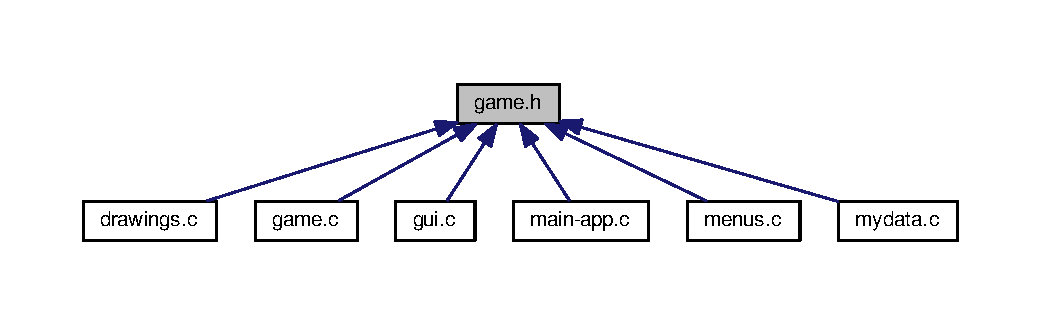
\includegraphics[width=350pt]{game_8h__dep__incl}
\end{center}
\end{figure}
\subsection*{Data Structures}
\begin{DoxyCompactItemize}
\item 
struct \hyperlink{struct_canon}{Canon}
\begin{DoxyCompactList}\small\item\em Objet contenant les informations pour un canon. \end{DoxyCompactList}\item 
struct \hyperlink{struct_shot}{Shot}
\begin{DoxyCompactList}\small\item\em Objet contenant les informations pour un shot. \end{DoxyCompactList}\item 
struct \hyperlink{struct_shot__list}{Shot\+\_\+list}
\begin{DoxyCompactList}\small\item\em Objet contenant les informations pour un \hyperlink{struct_shot__list}{Shot\+\_\+list}. \end{DoxyCompactList}\item 
struct \hyperlink{struct_marble}{Marble}
\begin{DoxyCompactList}\small\item\em Objet contenant les informations pour un \hyperlink{struct_marble}{Marble}. \end{DoxyCompactList}\item 
struct \hyperlink{struct_track}{Track}
\begin{DoxyCompactList}\small\item\em Objet contenant les informations pour un \hyperlink{struct_track}{Track}. \end{DoxyCompactList}\item 
struct \hyperlink{struct_track__list}{Track\+\_\+list}
\begin{DoxyCompactList}\small\item\em Objet contenant les informations pour un \hyperlink{struct_track__list}{Track\+\_\+list}. \end{DoxyCompactList}\item 
struct \hyperlink{struct_level}{Level}
\begin{DoxyCompactList}\small\item\em Objet contenant les informations pour un \hyperlink{struct_level}{Level}. \end{DoxyCompactList}\item 
struct \hyperlink{struct_level__list}{Level\+\_\+list}
\begin{DoxyCompactList}\small\item\em Objet contenant les informations pour un \hyperlink{struct_level__list}{Level\+\_\+list}. \end{DoxyCompactList}\item 
struct \hyperlink{struct_bonus}{Bonus}
\begin{DoxyCompactList}\small\item\em Objet contenant les informations pour un \hyperlink{struct_bonus}{Bonus}. \end{DoxyCompactList}\item 
struct \hyperlink{struct_game}{Game}
\begin{DoxyCompactList}\small\item\em Objet contenant les informations pour un \hyperlink{struct_game}{Game}. \end{DoxyCompactList}\end{DoxyCompactItemize}
\subsection*{Macros}
\begin{DoxyCompactItemize}
\item 
\#define {\bfseries S\+H\+O\+T\+\_\+\+M\+AX}~10\hypertarget{game_8h_ae8e233bf1b239802feef6bfb04a7070c}{}\label{game_8h_ae8e233bf1b239802feef6bfb04a7070c}

\item 
\#define {\bfseries S\+H\+O\+T\+\_\+\+S\+P\+E\+ED}~5\hypertarget{game_8h_af83d1d6d43a5093529db16c2ecbdde3f}{}\label{game_8h_af83d1d6d43a5093529db16c2ecbdde3f}

\item 
\#define {\bfseries T\+R\+A\+C\+K\+\_\+\+M\+AX}~10\hypertarget{game_8h_a94bd63d1de5cb3495fefbfbb9bfcb9c7}{}\label{game_8h_a94bd63d1de5cb3495fefbfbb9bfcb9c7}

\item 
\#define {\bfseries M\+A\+R\+B\+L\+E\+\_\+\+M\+A\+X\+\_\+\+A\+T\+\_\+\+S\+T\+A\+RT}~15\hypertarget{game_8h_a384017f042532c7ed5f4dd155ea8c682}{}\label{game_8h_a384017f042532c7ed5f4dd155ea8c682}

\item 
\#define {\bfseries M\+A\+R\+B\+L\+E\+\_\+\+M\+AX}~200\hypertarget{game_8h_ad1557f3fbb9abc1e447ed7eb7f871f97}{}\label{game_8h_ad1557f3fbb9abc1e447ed7eb7f871f97}

\item 
\#define {\bfseries S\+A\+M\+P\+L\+E\+\_\+\+M\+AX}~1000\hypertarget{game_8h_a82743e3343eacf1b8ba333e6d198b654}{}\label{game_8h_a82743e3343eacf1b8ba333e6d198b654}

\item 
\#define {\bfseries L\+E\+V\+E\+L\+\_\+\+M\+AX}~5\hypertarget{game_8h_a28e3d724c25aa80c53d9fef5d9dbad92}{}\label{game_8h_a28e3d724c25aa80c53d9fef5d9dbad92}

\item 
\#define {\bfseries S\+A\+M\+P\+L\+E\+\_\+\+T\+H\+E\+TA}~0.\+05\hypertarget{game_8h_a7ced8ead88267ac5c2ec17d5285271e4}{}\label{game_8h_a7ced8ead88267ac5c2ec17d5285271e4}

\item 
\#define {\bfseries M\+A\+R\+B\+L\+E\+\_\+\+S\+P\+E\+ED}~2\hypertarget{game_8h_a64625cb74e7eb968ef4e119425f02ec5}{}\label{game_8h_a64625cb74e7eb968ef4e119425f02ec5}

\item 
\#define {\bfseries M\+A\+R\+B\+L\+E\+\_\+\+S\+P\+E\+E\+D\+\_\+\+E\+N\+D\+\_\+\+G\+A\+ME}~10\hypertarget{game_8h_ac09ffdf66f0f1b753f8f06c40fb89f68}{}\label{game_8h_ac09ffdf66f0f1b753f8f06c40fb89f68}

\item 
\#define {\bfseries G\+A\+M\+E\+\_\+\+C\+A\+N\+N\+ON}~\char`\"{}canon.\+png\char`\"{}\hypertarget{game_8h_a579563ff4fbea898ab0e0aded7add7e9}{}\label{game_8h_a579563ff4fbea898ab0e0aded7add7e9}

\item 
\#define {\bfseries B\+O\+N\+U\+S\+\_\+\+T\+I\+ME}~5\hypertarget{game_8h_af1ffabafc06f0490b72fbb5398bc336e}{}\label{game_8h_af1ffabafc06f0490b72fbb5398bc336e}

\item 
\#define {\bfseries S\+C\+O\+R\+E\+\_\+\+P\+E\+N\+A\+L\+I\+TY}~5;\hypertarget{game_8h_a27f41dc9c0f5bdc09c2495b790a1c1be}{}\label{game_8h_a27f41dc9c0f5bdc09c2495b790a1c1be}

\end{DoxyCompactItemize}
\subsection*{Enumerations}
\begin{DoxyCompactItemize}
\item 
enum \hyperlink{game_8h_a33e243da48884e73997b5c5fa62864d4}{Game\+\_\+state} \{ \\*
{\bfseries G\+S\+\_\+\+H\+E\+L\+LO}, 
{\bfseries G\+S\+\_\+\+P\+L\+A\+Y\+I\+NG}, 
{\bfseries G\+S\+\_\+\+P\+A\+U\+SE}, 
{\bfseries G\+S\+\_\+\+W\+ON}, 
\\*
{\bfseries G\+S\+\_\+\+L\+O\+ST}
 \}\begin{DoxyCompactList}\small\item\em Constantes d\textquotesingle{}état du jeu. \end{DoxyCompactList}
\item 
enum \hyperlink{game_8h_a3d584d1e4b7b4c4a3cde3944c28fe594}{Track\+\_\+state} \{ {\bfseries T\+S\+\_\+\+I\+N\+T\+RO}, 
{\bfseries T\+S\+\_\+\+N\+O\+R\+M\+AL}, 
{\bfseries T\+S\+\_\+\+C\+O\+M\+B\+O2}, 
{\bfseries T\+S\+\_\+\+C\+O\+M\+B\+O3}
 \}\begin{DoxyCompactList}\small\item\em Constantes d\textquotesingle{}état de la track. \end{DoxyCompactList}
\item 
enum \hyperlink{game_8h_af6e7be305743e35f65003ee68d02f6f5}{Ammo\+Color} \{ \\*
{\bfseries R\+ED}, 
{\bfseries G\+R\+E\+EN}, 
{\bfseries B\+L\+UE}, 
{\bfseries Y\+E\+L\+L\+OW}, 
\\*
{\bfseries P\+U\+R\+P\+LE}, 
{\bfseries I\+N\+D\+I\+GO}, 
{\bfseries L\+A\+S\+T\+\_\+\+C\+O\+L\+OR}
 \}\begin{DoxyCompactList}\small\item\em Constantes des couleurs. \end{DoxyCompactList}
\item 
enum \hyperlink{game_8h_a7b2ac2fd4d85740443adc95ada0f4784}{Bonus\+\_\+state} \{ \\*
{\bfseries B\+S\+\_\+\+N\+O\+NE}, 
{\bfseries B\+S\+\_\+\+T\+I\+M\+E\+\_\+\+S\+T\+OP}, 
{\bfseries B\+S\+\_\+\+T\+I\+M\+E\+\_\+\+S\+L\+O\+W\+ER}, 
{\bfseries B\+S\+\_\+\+T\+I\+M\+E\+\_\+\+F\+A\+S\+T\+ER}, 
\\*
{\bfseries B\+S\+\_\+\+M\+A\+R\+B\+L\+E\+\_\+\+E\+X\+P\+L\+O\+S\+I\+VE}
 \}\begin{DoxyCompactList}\small\item\em Constantes des bonus. \end{DoxyCompactList}
\end{DoxyCompactItemize}
\subsection*{Functions}
\begin{DoxyCompactItemize}
\item 
void \hyperlink{game_8h_a1379e442012bd2db4e0a7c43ba12a140}{sample\+\_\+curve\+\_\+to\+\_\+track} (\hyperlink{struct_curve}{Curve} $\ast$curve, \hyperlink{struct_track}{Track} $\ast$track, double theta)
\begin{DoxyCompactList}\small\item\em Fonction de conversion d\textquotesingle{}une curve en une track. \end{DoxyCompactList}\item 
void {\bfseries shoot\+\_\+ammo} (\hyperlink{struct_game}{Game} $\ast$game)\hypertarget{game_8h_a7a28065cd246ecccf78c7b940b4b6651}{}\label{game_8h_a7a28065cd246ecccf78c7b940b4b6651}

\item 
int \hyperlink{game_8h_a32dbc2ae6d9dd615b664c16ef04bf376}{is\+\_\+color\+\_\+on\+\_\+track} (\hyperlink{struct_track}{Track} $\ast$track, int color)
\begin{DoxyCompactList}\small\item\em Fonction pour chercher si une couleur est dans la track. \end{DoxyCompactList}\item 
void \hyperlink{game_8h_aaf45176a520f6cfd9d8a52c140802a5d}{prepare\+\_\+ammo} (\hyperlink{struct_game}{Game} $\ast$game)
\begin{DoxyCompactList}\small\item\em Fonction pour préparer les balles du canon après un tir. \end{DoxyCompactList}\item 
void \hyperlink{game_8h_a561e64089b963fcb06eff3c654bc8585}{swap\+\_\+ammo} (\hyperlink{struct_game}{Game} $\ast$game)
\begin{DoxyCompactList}\small\item\em Fonction pour echanger les balles du canon. \end{DoxyCompactList}\item 
void \hyperlink{game_8h_a321533d866fea72c822dabdeb0ccc094}{game\+\_\+pause} (\hyperlink{struct_game}{Game} $\ast$game)
\begin{DoxyCompactList}\small\item\em Fonction pour mettre en pause le jeu si il ne l\textquotesingle{}est pas sinon le remet en mode playing. \end{DoxyCompactList}\item 
int \hyperlink{game_8h_ab883e1857818d6661a3af2fa4843536f}{calcule\+\_\+score\+\_\+with\+\_\+marble\+\_\+group\+\_\+size} (\hyperlink{struct_game}{Game} $\ast$game, \hyperlink{struct_track}{Track} $\ast$track, int marble\+\_\+id\+\_\+start, int score, int bonus)
\begin{DoxyCompactList}\small\item\em Fonction pour calculer le score obtenu après un tir. \end{DoxyCompactList}\item 
void \hyperlink{game_8h_a6a5803be3dedb50a82b3d625ac90ea3e}{check\+\_\+bonus} (\hyperlink{struct_game}{Game} $\ast$game, \hyperlink{struct_track}{Track} $\ast$track, int marble)
\begin{DoxyCompactList}\small\item\em Fonction pour vérifier si il y a un bonus. \end{DoxyCompactList}\item 
void \hyperlink{game_8h_a171ea500d411c5194613976786047d70}{check\+\_\+bonus\+\_\+end} (\hyperlink{struct_game}{Game} $\ast$game)
\begin{DoxyCompactList}\small\item\em Fonction pour vérifier un bonus est terminé \end{DoxyCompactList}\item 
void \hyperlink{game_8h_a4476eab4b74a53b36cdf7d7096c62060}{move\+\_\+shots\+\_\+one\+\_\+step} (\hyperlink{struct_game}{Game} $\ast$game)
\begin{DoxyCompactList}\small\item\em Fonction pour avancer le shot. \end{DoxyCompactList}\item 
void \hyperlink{game_8h_a401c25af3ee1e41a353329513c7fb679}{suppress\+\_\+far\+\_\+shots} (\hyperlink{struct_game}{Game} $\ast$game, int screen\+\_\+width, int screen\+\_\+height)
\begin{DoxyCompactList}\small\item\em Fonction de suppression des tirs lointains. \end{DoxyCompactList}\item 
void \hyperlink{game_8h_a590c19b4c7fbc37e84976b4d3773e0b7}{do\+\_\+vector\+\_\+product} (double xu, double yu, double zu, double xv, double yv, double zv, double $\ast$x, double $\ast$y, double $\ast$z)
\item 
int \hyperlink{game_8h_a868a0d63645e599dd01aee704da37251}{test\+\_\+collision} (\hyperlink{struct_game}{Game} $\ast$game, int $\ast$shot\+\_\+num, int $\ast$marble\+\_\+num, int track\+\_\+num)
\begin{DoxyCompactList}\small\item\em fonctione pour tester si il y a une colision entre un shot et une bille du train \end{DoxyCompactList}\item 
void \hyperlink{game_8h_a903a06d0784febcd3fdcf811cc71a28f}{process\+\_\+shots\+\_\+collisions} (\hyperlink{struct_game}{Game} $\ast$game)
\begin{DoxyCompactList}\small\item\em insertion de la bille si il y a eu colision \end{DoxyCompactList}\item 
void \hyperlink{game_8h_a82438caca3314471bef10e102441af12}{move\+\_\+trains\+\_\+one\+\_\+step} (\hyperlink{struct_game}{Game} $\ast$game)
\begin{DoxyCompactList}\small\item\em Fonction pour faire avancer le train. \end{DoxyCompactList}\item 
void \hyperlink{game_8h_aa5da90408ff8ede3b09fa6a0a376c709}{check\+\_\+end\+\_\+of\+\_\+game} (\hyperlink{struct_game}{Game} $\ast$game)
\begin{DoxyCompactList}\small\item\em Fonction pour vérifier si la partie est terminé \end{DoxyCompactList}\item 
void \hyperlink{game_8h_a5b35e1416156b7ae084045350ba89ab9}{progress\+\_\+game\+\_\+next\+\_\+step} (\hyperlink{struct_game}{Game} $\ast$game, int screen\+\_\+width, int screen\+\_\+height)
\begin{DoxyCompactList}\small\item\em Fonction d\textquotesingle{}étape du jeu (boucle principale) \end{DoxyCompactList}\item 
void \hyperlink{game_8h_a737ca8731777960973c03c78e1d777d7}{update\+\_\+x\+\_\+and\+\_\+y\+\_\+canon} (\hyperlink{struct_game}{Game} $\ast$game, int height, int width)
\begin{DoxyCompactList}\small\item\em Fonction de mise à jour de la postion du canon par rapport à l\textquotesingle{}écran pour le centrer. \end{DoxyCompactList}\item 
void \hyperlink{game_8h_a5c95bbb5adb20ea2cbf4ed0bc1c9025f}{load\+\_\+cannon\+\_\+image} (\hyperlink{struct_game}{Game} $\ast$game)
\begin{DoxyCompactList}\small\item\em Fonction pour charger l\textquotesingle{}image du canon. \end{DoxyCompactList}\item 
void \hyperlink{game_8h_adad209d500c35da1b3d4985e7a09bec4}{update\+\_\+canon\+\_\+angle} (\hyperlink{struct_game}{Game} $\ast$game, double sx, double sy)
\begin{DoxyCompactList}\small\item\em Fonction pour mettre à jour l\textquotesingle{}angle du canon. \end{DoxyCompactList}\item 
void \hyperlink{game_8h_aa832339540d987f842a7d505da20803c}{init\+\_\+canon} (\hyperlink{struct_game}{Game} $\ast$game, int height, int width)
\begin{DoxyCompactList}\small\item\em Fonction pour l\textquotesingle{}initialisation du canon. \end{DoxyCompactList}\item 
void \hyperlink{game_8h_afd103f2ed5a4accadde77c8f8fbe489b}{init\+\_\+ammo} (\hyperlink{struct_game}{Game} $\ast$game)
\begin{DoxyCompactList}\small\item\em Fonction pour l\textquotesingle{}initialisation des munitions du canon. \end{DoxyCompactList}\item 
void \hyperlink{game_8h_a76bc3a19eb94631d39401b92e638d529}{init\+\_\+shots} (\hyperlink{struct_game}{Game} $\ast$game)
\begin{DoxyCompactList}\small\item\em Fonction pour l\textquotesingle{}initialisation des shots. \end{DoxyCompactList}\item 
int \hyperlink{game_8h_aec4660f64205ee890c1c609f7883cd16}{init\+\_\+marble\+\_\+bonus} ()
\begin{DoxyCompactList}\small\item\em Fonction pour la génération du bonus aléatoirement. \end{DoxyCompactList}\item 
void \hyperlink{game_8h_a090892ad996749a780a8f8c7670a853d}{create\+\_\+marbles} (\hyperlink{struct_track}{Track} $\ast$track, int current\+\_\+level)
\begin{DoxyCompactList}\small\item\em Fonction pour créer les billes. \end{DoxyCompactList}\item 
void \hyperlink{game_8h_af1c8645a911806b783052f96c2f9f96d}{init\+\_\+track} (\hyperlink{struct_game}{Game} $\ast$game)
\begin{DoxyCompactList}\small\item\em Fonction pour l\textquotesingle{}initialisation de la track. \end{DoxyCompactList}\item 
void \hyperlink{game_8h_a1aa823f431873e33d5b7095aaf8199f8}{init\+\_\+game} (\hyperlink{struct_game}{Game} $\ast$game, int height, int width)
\begin{DoxyCompactList}\small\item\em Fonction pour l\textquotesingle{}initialisation du jeu. \end{DoxyCompactList}\item 
void \hyperlink{game_8h_a96baae852b652337739b9cf463ec9a5f}{reset\+\_\+game} (\hyperlink{struct_game}{Game} $\ast$game, int height, int width)
\begin{DoxyCompactList}\small\item\em Fonction de réinitialisation du jeu. \end{DoxyCompactList}\item 
void \hyperlink{game_8h_a971b5b9e0391b68e00546b19fe07bafb}{restart\+\_\+game} (\hyperlink{struct_game}{Game} $\ast$game, int height, int width)
\begin{DoxyCompactList}\small\item\em Fonction pour recommencer un level. \end{DoxyCompactList}\item 
void \hyperlink{game_8h_a055ce2874a0fbed77092e4ba81c59ddf}{change\+\_\+level} (\hyperlink{struct_game}{Game} $\ast$game, int height, int width)
\begin{DoxyCompactList}\small\item\em Fonction pour changer de level. \end{DoxyCompactList}\item 
void \hyperlink{game_8h_ab5fc2f364ae1501956a2958de19cbe97}{time\+\_\+stop} (\hyperlink{struct_game}{Game} $\ast$game)
\begin{DoxyCompactList}\small\item\em Fonction pour arrêter le temps ( le train) \end{DoxyCompactList}\item 
void \hyperlink{game_8h_ad88ea8e0d2afe0c3987e18e586274c1b}{speed\+\_\+change} (\hyperlink{struct_game}{Game} $\ast$game, int bonus)
\begin{DoxyCompactList}\small\item\em Fonction pour changer la vitesse du train, accélérer ou bien ralentir. \end{DoxyCompactList}\end{DoxyCompactItemize}


\subsection{Detailed Description}
Fonctions et objets principaux du jeu. 

\begin{DoxyAuthor}{Author}
Gaëtan Perrot 
\end{DoxyAuthor}
\begin{DoxyVersion}{Version}
0.\+1 
\end{DoxyVersion}
\begin{DoxyDate}{Date}
23 avril 2017
\end{DoxyDate}
Fonctions et objets principaux du jeu 

\subsection{Enumeration Type Documentation}
\index{game.\+h@{game.\+h}!Ammo\+Color@{Ammo\+Color}}
\index{Ammo\+Color@{Ammo\+Color}!game.\+h@{game.\+h}}
\subsubsection[{\texorpdfstring{Ammo\+Color}{AmmoColor}}]{\setlength{\rightskip}{0pt plus 5cm}enum {\bf Ammo\+Color}}\hypertarget{game_8h_af6e7be305743e35f65003ee68d02f6f5}{}\label{game_8h_af6e7be305743e35f65003ee68d02f6f5}


Constantes des couleurs. 

Ammo\+Color est une série de constantes prédéfinie pour la gestion des couleurs \index{game.\+h@{game.\+h}!Bonus\+\_\+state@{Bonus\+\_\+state}}
\index{Bonus\+\_\+state@{Bonus\+\_\+state}!game.\+h@{game.\+h}}
\subsubsection[{\texorpdfstring{Bonus\+\_\+state}{Bonus_state}}]{\setlength{\rightskip}{0pt plus 5cm}enum {\bf Bonus\+\_\+state}}\hypertarget{game_8h_a7b2ac2fd4d85740443adc95ada0f4784}{}\label{game_8h_a7b2ac2fd4d85740443adc95ada0f4784}


Constantes des bonus. 

Bonus\+\_\+state est une série de constantes prédéfinie pour la gestion des bonus \index{game.\+h@{game.\+h}!Game\+\_\+state@{Game\+\_\+state}}
\index{Game\+\_\+state@{Game\+\_\+state}!game.\+h@{game.\+h}}
\subsubsection[{\texorpdfstring{Game\+\_\+state}{Game_state}}]{\setlength{\rightskip}{0pt plus 5cm}enum {\bf Game\+\_\+state}}\hypertarget{game_8h_a33e243da48884e73997b5c5fa62864d4}{}\label{game_8h_a33e243da48884e73997b5c5fa62864d4}


Constantes d\textquotesingle{}état du jeu. 

Game\+\_\+state est une série de constantes prédéfinie pour la gestion d\textquotesingle{}état du jeu. \index{game.\+h@{game.\+h}!Track\+\_\+state@{Track\+\_\+state}}
\index{Track\+\_\+state@{Track\+\_\+state}!game.\+h@{game.\+h}}
\subsubsection[{\texorpdfstring{Track\+\_\+state}{Track_state}}]{\setlength{\rightskip}{0pt plus 5cm}enum {\bf Track\+\_\+state}}\hypertarget{game_8h_a3d584d1e4b7b4c4a3cde3944c28fe594}{}\label{game_8h_a3d584d1e4b7b4c4a3cde3944c28fe594}


Constantes d\textquotesingle{}état de la track. 

Track\+\_\+state est une série de constantes prédéfinie pour la gestion d\textquotesingle{}état de la track. 

\subsection{Function Documentation}
\index{game.\+h@{game.\+h}!calcule\+\_\+score\+\_\+with\+\_\+marble\+\_\+group\+\_\+size@{calcule\+\_\+score\+\_\+with\+\_\+marble\+\_\+group\+\_\+size}}
\index{calcule\+\_\+score\+\_\+with\+\_\+marble\+\_\+group\+\_\+size@{calcule\+\_\+score\+\_\+with\+\_\+marble\+\_\+group\+\_\+size}!game.\+h@{game.\+h}}
\subsubsection[{\texorpdfstring{calcule\+\_\+score\+\_\+with\+\_\+marble\+\_\+group\+\_\+size(\+Game $\ast$game, Track $\ast$track, int marble\+\_\+id\+\_\+start, int score, int bonus)}{calcule_score_with_marble_group_size(Game *game, Track *track, int marble_id_start, int score, int bonus)}}]{\setlength{\rightskip}{0pt plus 5cm}int calcule\+\_\+score\+\_\+with\+\_\+marble\+\_\+group\+\_\+size (
\begin{DoxyParamCaption}
\item[{{\bf Game} $\ast$}]{game, }
\item[{{\bf Track} $\ast$}]{track, }
\item[{int}]{marble\+\_\+id\+\_\+start, }
\item[{int}]{score, }
\item[{int}]{combo}
\end{DoxyParamCaption}
)}\hypertarget{game_8h_ab883e1857818d6661a3af2fa4843536f}{}\label{game_8h_ab883e1857818d6661a3af2fa4843536f}


Fonction pour calculer le score obtenu après un tir. 


\begin{DoxyParams}{Parameters}
{\em self} & Objet \hyperlink{struct_game}{Game} $\ast$ game,\hyperlink{struct_track}{Track} $\ast$ track, int marble\+\_\+id\+\_\+start,int score,int bonus \\
\hline
\end{DoxyParams}
\begin{DoxyReturn}{Returns}
int 
\end{DoxyReturn}
\index{game.\+h@{game.\+h}!change\+\_\+level@{change\+\_\+level}}
\index{change\+\_\+level@{change\+\_\+level}!game.\+h@{game.\+h}}
\subsubsection[{\texorpdfstring{change\+\_\+level(\+Game $\ast$game, int height, int width)}{change_level(Game *game, int height, int width)}}]{\setlength{\rightskip}{0pt plus 5cm}void change\+\_\+level (
\begin{DoxyParamCaption}
\item[{{\bf Game} $\ast$}]{game, }
\item[{int}]{height, }
\item[{int}]{width}
\end{DoxyParamCaption}
)}\hypertarget{game_8h_a055ce2874a0fbed77092e4ba81c59ddf}{}\label{game_8h_a055ce2874a0fbed77092e4ba81c59ddf}


Fonction pour changer de level. 


\begin{DoxyParams}{Parameters}
{\em self} & \hyperlink{struct_game}{Game} $\ast$ game, int height, int width \\
\hline
\end{DoxyParams}
\begin{DoxyReturn}{Returns}
void 
\end{DoxyReturn}
\index{game.\+h@{game.\+h}!check\+\_\+bonus@{check\+\_\+bonus}}
\index{check\+\_\+bonus@{check\+\_\+bonus}!game.\+h@{game.\+h}}
\subsubsection[{\texorpdfstring{check\+\_\+bonus(\+Game $\ast$game, Track $\ast$track, int marble)}{check_bonus(Game *game, Track *track, int marble)}}]{\setlength{\rightskip}{0pt plus 5cm}void check\+\_\+bonus (
\begin{DoxyParamCaption}
\item[{{\bf Game} $\ast$}]{game, }
\item[{{\bf Track} $\ast$}]{track, }
\item[{int}]{marble}
\end{DoxyParamCaption}
)}\hypertarget{game_8h_a6a5803be3dedb50a82b3d625ac90ea3e}{}\label{game_8h_a6a5803be3dedb50a82b3d625ac90ea3e}


Fonction pour vérifier si il y a un bonus. 


\begin{DoxyParams}{Parameters}
{\em self} & Objet \hyperlink{struct_game}{Game} $\ast$ game,\hyperlink{struct_track}{Track} $\ast$ track,int marble \\
\hline
\end{DoxyParams}
\begin{DoxyReturn}{Returns}
void 
\end{DoxyReturn}
\index{game.\+h@{game.\+h}!check\+\_\+bonus\+\_\+end@{check\+\_\+bonus\+\_\+end}}
\index{check\+\_\+bonus\+\_\+end@{check\+\_\+bonus\+\_\+end}!game.\+h@{game.\+h}}
\subsubsection[{\texorpdfstring{check\+\_\+bonus\+\_\+end(\+Game $\ast$game)}{check_bonus_end(Game *game)}}]{\setlength{\rightskip}{0pt plus 5cm}void check\+\_\+bonus\+\_\+end (
\begin{DoxyParamCaption}
\item[{{\bf Game} $\ast$}]{game}
\end{DoxyParamCaption}
)}\hypertarget{game_8h_a171ea500d411c5194613976786047d70}{}\label{game_8h_a171ea500d411c5194613976786047d70}


Fonction pour vérifier un bonus est terminé 


\begin{DoxyParams}{Parameters}
{\em self} & Objet \hyperlink{struct_game}{Game} \\
\hline
\end{DoxyParams}
\begin{DoxyReturn}{Returns}
void 
\end{DoxyReturn}
\index{game.\+h@{game.\+h}!check\+\_\+end\+\_\+of\+\_\+game@{check\+\_\+end\+\_\+of\+\_\+game}}
\index{check\+\_\+end\+\_\+of\+\_\+game@{check\+\_\+end\+\_\+of\+\_\+game}!game.\+h@{game.\+h}}
\subsubsection[{\texorpdfstring{check\+\_\+end\+\_\+of\+\_\+game(\+Game $\ast$game)}{check_end_of_game(Game *game)}}]{\setlength{\rightskip}{0pt plus 5cm}void check\+\_\+end\+\_\+of\+\_\+game (
\begin{DoxyParamCaption}
\item[{{\bf Game} $\ast$}]{game}
\end{DoxyParamCaption}
)}\hypertarget{game_8h_aa5da90408ff8ede3b09fa6a0a376c709}{}\label{game_8h_aa5da90408ff8ede3b09fa6a0a376c709}


Fonction pour vérifier si la partie est terminé 


\begin{DoxyParams}{Parameters}
{\em self} & \hyperlink{struct_game}{Game} $\ast$ game \\
\hline
\end{DoxyParams}
\begin{DoxyReturn}{Returns}
void 
\end{DoxyReturn}
\index{game.\+h@{game.\+h}!create\+\_\+marbles@{create\+\_\+marbles}}
\index{create\+\_\+marbles@{create\+\_\+marbles}!game.\+h@{game.\+h}}
\subsubsection[{\texorpdfstring{create\+\_\+marbles(\+Track $\ast$track, int current\+\_\+level)}{create_marbles(Track *track, int current_level)}}]{\setlength{\rightskip}{0pt plus 5cm}void create\+\_\+marbles (
\begin{DoxyParamCaption}
\item[{{\bf Track} $\ast$}]{track, }
\item[{int}]{current\+\_\+level}
\end{DoxyParamCaption}
)}\hypertarget{game_8h_a090892ad996749a780a8f8c7670a853d}{}\label{game_8h_a090892ad996749a780a8f8c7670a853d}


Fonction pour créer les billes. 


\begin{DoxyParams}{Parameters}
{\em self} & \hyperlink{struct_track}{Track} $\ast$ track,int current\+\_\+level \\
\hline
\end{DoxyParams}
\begin{DoxyReturn}{Returns}
void 
\end{DoxyReturn}
\index{game.\+h@{game.\+h}!do\+\_\+vector\+\_\+product@{do\+\_\+vector\+\_\+product}}
\index{do\+\_\+vector\+\_\+product@{do\+\_\+vector\+\_\+product}!game.\+h@{game.\+h}}
\subsubsection[{\texorpdfstring{do\+\_\+vector\+\_\+product(double xu, double yu, double zu, double xv, double yv, double zv, double $\ast$x, double $\ast$y, double $\ast$z)}{do_vector_product(double xu, double yu, double zu, double xv, double yv, double zv, double *x, double *y, double *z)}}]{\setlength{\rightskip}{0pt plus 5cm}void do\+\_\+vector\+\_\+product (
\begin{DoxyParamCaption}
\item[{double}]{xu, }
\item[{double}]{yu, }
\item[{double}]{zu, }
\item[{double}]{xv, }
\item[{double}]{yv, }
\item[{double}]{zv, }
\item[{double $\ast$}]{x, }
\item[{double $\ast$}]{y, }
\item[{double $\ast$}]{z}
\end{DoxyParamCaption}
)}\hypertarget{game_8h_a590c19b4c7fbc37e84976b4d3773e0b7}{}\label{game_8h_a590c19b4c7fbc37e84976b4d3773e0b7}

\begin{DoxyParams}{Parameters}
{\em self} & double xu,double yu,double zu,double xv,double yv,double zv, double $\ast$x, double $\ast$y,double $\ast$z) \\
\hline
\end{DoxyParams}
\begin{DoxyReturn}{Returns}
void 
\end{DoxyReturn}
\index{game.\+h@{game.\+h}!game\+\_\+pause@{game\+\_\+pause}}
\index{game\+\_\+pause@{game\+\_\+pause}!game.\+h@{game.\+h}}
\subsubsection[{\texorpdfstring{game\+\_\+pause(\+Game $\ast$game)}{game_pause(Game *game)}}]{\setlength{\rightskip}{0pt plus 5cm}void game\+\_\+pause (
\begin{DoxyParamCaption}
\item[{{\bf Game} $\ast$}]{game}
\end{DoxyParamCaption}
)}\hypertarget{game_8h_a321533d866fea72c822dabdeb0ccc094}{}\label{game_8h_a321533d866fea72c822dabdeb0ccc094}


Fonction pour mettre en pause le jeu si il ne l\textquotesingle{}est pas sinon le remet en mode playing. 


\begin{DoxyParams}{Parameters}
{\em self} & Objet \hyperlink{struct_game}{Game} \\
\hline
\end{DoxyParams}
\begin{DoxyReturn}{Returns}
void 
\end{DoxyReturn}
\index{game.\+h@{game.\+h}!init\+\_\+ammo@{init\+\_\+ammo}}
\index{init\+\_\+ammo@{init\+\_\+ammo}!game.\+h@{game.\+h}}
\subsubsection[{\texorpdfstring{init\+\_\+ammo(\+Game $\ast$game)}{init_ammo(Game *game)}}]{\setlength{\rightskip}{0pt plus 5cm}void init\+\_\+ammo (
\begin{DoxyParamCaption}
\item[{{\bf Game} $\ast$}]{game}
\end{DoxyParamCaption}
)}\hypertarget{game_8h_afd103f2ed5a4accadde77c8f8fbe489b}{}\label{game_8h_afd103f2ed5a4accadde77c8f8fbe489b}


Fonction pour l\textquotesingle{}initialisation des munitions du canon. 


\begin{DoxyParams}{Parameters}
{\em self} & \hyperlink{struct_game}{Game} $\ast$ game \\
\hline
\end{DoxyParams}
\begin{DoxyReturn}{Returns}
void 
\end{DoxyReturn}
\index{game.\+h@{game.\+h}!init\+\_\+canon@{init\+\_\+canon}}
\index{init\+\_\+canon@{init\+\_\+canon}!game.\+h@{game.\+h}}
\subsubsection[{\texorpdfstring{init\+\_\+canon(\+Game $\ast$game, int height, int width)}{init_canon(Game *game, int height, int width)}}]{\setlength{\rightskip}{0pt plus 5cm}void init\+\_\+canon (
\begin{DoxyParamCaption}
\item[{{\bf Game} $\ast$}]{game, }
\item[{int}]{height, }
\item[{int}]{width}
\end{DoxyParamCaption}
)}\hypertarget{game_8h_aa832339540d987f842a7d505da20803c}{}\label{game_8h_aa832339540d987f842a7d505da20803c}


Fonction pour l\textquotesingle{}initialisation du canon. 


\begin{DoxyParams}{Parameters}
{\em self} & \hyperlink{struct_game}{Game} $\ast$ game,int height, int width \\
\hline
\end{DoxyParams}
\begin{DoxyReturn}{Returns}
void 
\end{DoxyReturn}
\index{game.\+h@{game.\+h}!init\+\_\+game@{init\+\_\+game}}
\index{init\+\_\+game@{init\+\_\+game}!game.\+h@{game.\+h}}
\subsubsection[{\texorpdfstring{init\+\_\+game(\+Game $\ast$game, int height, int width)}{init_game(Game *game, int height, int width)}}]{\setlength{\rightskip}{0pt plus 5cm}void init\+\_\+game (
\begin{DoxyParamCaption}
\item[{{\bf Game} $\ast$}]{game, }
\item[{int}]{height, }
\item[{int}]{width}
\end{DoxyParamCaption}
)}\hypertarget{game_8h_a1aa823f431873e33d5b7095aaf8199f8}{}\label{game_8h_a1aa823f431873e33d5b7095aaf8199f8}


Fonction pour l\textquotesingle{}initialisation du jeu. 


\begin{DoxyParams}{Parameters}
{\em self} & \hyperlink{struct_game}{Game} $\ast$ game, int height, int width \\
\hline
\end{DoxyParams}
\begin{DoxyReturn}{Returns}
void 
\end{DoxyReturn}
\index{game.\+h@{game.\+h}!init\+\_\+marble\+\_\+bonus@{init\+\_\+marble\+\_\+bonus}}
\index{init\+\_\+marble\+\_\+bonus@{init\+\_\+marble\+\_\+bonus}!game.\+h@{game.\+h}}
\subsubsection[{\texorpdfstring{init\+\_\+marble\+\_\+bonus()}{init_marble_bonus()}}]{\setlength{\rightskip}{0pt plus 5cm}int init\+\_\+marble\+\_\+bonus (
\begin{DoxyParamCaption}
{}
\end{DoxyParamCaption}
)}\hypertarget{game_8h_aec4660f64205ee890c1c609f7883cd16}{}\label{game_8h_aec4660f64205ee890c1c609f7883cd16}


Fonction pour la génération du bonus aléatoirement. 


\begin{DoxyParams}{Parameters}
{\em self} & \\
\hline
\end{DoxyParams}
\begin{DoxyReturn}{Returns}
int le bonus généré aléatoirement 
\end{DoxyReturn}
\index{game.\+h@{game.\+h}!init\+\_\+shots@{init\+\_\+shots}}
\index{init\+\_\+shots@{init\+\_\+shots}!game.\+h@{game.\+h}}
\subsubsection[{\texorpdfstring{init\+\_\+shots(\+Game $\ast$game)}{init_shots(Game *game)}}]{\setlength{\rightskip}{0pt plus 5cm}void init\+\_\+shots (
\begin{DoxyParamCaption}
\item[{{\bf Game} $\ast$}]{game}
\end{DoxyParamCaption}
)}\hypertarget{game_8h_a76bc3a19eb94631d39401b92e638d529}{}\label{game_8h_a76bc3a19eb94631d39401b92e638d529}


Fonction pour l\textquotesingle{}initialisation des shots. 


\begin{DoxyParams}{Parameters}
{\em self} & \hyperlink{struct_game}{Game} $\ast$ game \\
\hline
\end{DoxyParams}
\begin{DoxyReturn}{Returns}
void 
\end{DoxyReturn}
\index{game.\+h@{game.\+h}!init\+\_\+track@{init\+\_\+track}}
\index{init\+\_\+track@{init\+\_\+track}!game.\+h@{game.\+h}}
\subsubsection[{\texorpdfstring{init\+\_\+track(\+Game $\ast$game)}{init_track(Game *game)}}]{\setlength{\rightskip}{0pt plus 5cm}void init\+\_\+track (
\begin{DoxyParamCaption}
\item[{{\bf Game} $\ast$}]{game}
\end{DoxyParamCaption}
)}\hypertarget{game_8h_af1c8645a911806b783052f96c2f9f96d}{}\label{game_8h_af1c8645a911806b783052f96c2f9f96d}


Fonction pour l\textquotesingle{}initialisation de la track. 


\begin{DoxyParams}{Parameters}
{\em self} & \hyperlink{struct_game}{Game} $\ast$ game \\
\hline
\end{DoxyParams}
\begin{DoxyReturn}{Returns}
void 
\end{DoxyReturn}
\index{game.\+h@{game.\+h}!is\+\_\+color\+\_\+on\+\_\+track@{is\+\_\+color\+\_\+on\+\_\+track}}
\index{is\+\_\+color\+\_\+on\+\_\+track@{is\+\_\+color\+\_\+on\+\_\+track}!game.\+h@{game.\+h}}
\subsubsection[{\texorpdfstring{is\+\_\+color\+\_\+on\+\_\+track(\+Track $\ast$track, int color)}{is_color_on_track(Track *track, int color)}}]{\setlength{\rightskip}{0pt plus 5cm}int is\+\_\+color\+\_\+on\+\_\+track (
\begin{DoxyParamCaption}
\item[{{\bf Track} $\ast$}]{track, }
\item[{int}]{color}
\end{DoxyParamCaption}
)}\hypertarget{game_8h_a32dbc2ae6d9dd615b664c16ef04bf376}{}\label{game_8h_a32dbc2ae6d9dd615b664c16ef04bf376}


Fonction pour chercher si une couleur est dans la track. 


\begin{DoxyParams}{Parameters}
{\em self} & Objet \hyperlink{struct_track}{Track} $\ast$ track, int color \\
\hline
\end{DoxyParams}
\begin{DoxyReturn}{Returns}
retourne 1 si la couleur est déjà dans la track et 0 si elle ne l\textquotesingle{}ait pas 
\end{DoxyReturn}
\index{game.\+h@{game.\+h}!load\+\_\+cannon\+\_\+image@{load\+\_\+cannon\+\_\+image}}
\index{load\+\_\+cannon\+\_\+image@{load\+\_\+cannon\+\_\+image}!game.\+h@{game.\+h}}
\subsubsection[{\texorpdfstring{load\+\_\+cannon\+\_\+image(\+Game $\ast$game)}{load_cannon_image(Game *game)}}]{\setlength{\rightskip}{0pt plus 5cm}void load\+\_\+cannon\+\_\+image (
\begin{DoxyParamCaption}
\item[{{\bf Game} $\ast$}]{game}
\end{DoxyParamCaption}
)}\hypertarget{game_8h_a5c95bbb5adb20ea2cbf4ed0bc1c9025f}{}\label{game_8h_a5c95bbb5adb20ea2cbf4ed0bc1c9025f}


Fonction pour charger l\textquotesingle{}image du canon. 


\begin{DoxyParams}{Parameters}
{\em self} & \hyperlink{struct_game}{Game} $\ast$ game \\
\hline
\end{DoxyParams}
\begin{DoxyReturn}{Returns}
void 
\end{DoxyReturn}
\index{game.\+h@{game.\+h}!move\+\_\+shots\+\_\+one\+\_\+step@{move\+\_\+shots\+\_\+one\+\_\+step}}
\index{move\+\_\+shots\+\_\+one\+\_\+step@{move\+\_\+shots\+\_\+one\+\_\+step}!game.\+h@{game.\+h}}
\subsubsection[{\texorpdfstring{move\+\_\+shots\+\_\+one\+\_\+step(\+Game $\ast$game)}{move_shots_one_step(Game *game)}}]{\setlength{\rightskip}{0pt plus 5cm}void move\+\_\+shots\+\_\+one\+\_\+step (
\begin{DoxyParamCaption}
\item[{{\bf Game} $\ast$}]{game}
\end{DoxyParamCaption}
)}\hypertarget{game_8h_a4476eab4b74a53b36cdf7d7096c62060}{}\label{game_8h_a4476eab4b74a53b36cdf7d7096c62060}


Fonction pour avancer le shot. 


\begin{DoxyParams}{Parameters}
{\em self} & Objet \hyperlink{struct_game}{Game} \\
\hline
\end{DoxyParams}
\begin{DoxyReturn}{Returns}
void 
\end{DoxyReturn}
\index{game.\+h@{game.\+h}!move\+\_\+trains\+\_\+one\+\_\+step@{move\+\_\+trains\+\_\+one\+\_\+step}}
\index{move\+\_\+trains\+\_\+one\+\_\+step@{move\+\_\+trains\+\_\+one\+\_\+step}!game.\+h@{game.\+h}}
\subsubsection[{\texorpdfstring{move\+\_\+trains\+\_\+one\+\_\+step(\+Game $\ast$game)}{move_trains_one_step(Game *game)}}]{\setlength{\rightskip}{0pt plus 5cm}void move\+\_\+trains\+\_\+one\+\_\+step (
\begin{DoxyParamCaption}
\item[{{\bf Game} $\ast$}]{game}
\end{DoxyParamCaption}
)}\hypertarget{game_8h_a82438caca3314471bef10e102441af12}{}\label{game_8h_a82438caca3314471bef10e102441af12}


Fonction pour faire avancer le train. 


\begin{DoxyParams}{Parameters}
{\em self} & \hyperlink{struct_game}{Game} $\ast$ game \\
\hline
\end{DoxyParams}
\begin{DoxyReturn}{Returns}
void 
\end{DoxyReturn}
\index{game.\+h@{game.\+h}!prepare\+\_\+ammo@{prepare\+\_\+ammo}}
\index{prepare\+\_\+ammo@{prepare\+\_\+ammo}!game.\+h@{game.\+h}}
\subsubsection[{\texorpdfstring{prepare\+\_\+ammo(\+Game $\ast$game)}{prepare_ammo(Game *game)}}]{\setlength{\rightskip}{0pt plus 5cm}void prepare\+\_\+ammo (
\begin{DoxyParamCaption}
\item[{{\bf Game} $\ast$}]{game}
\end{DoxyParamCaption}
)}\hypertarget{game_8h_aaf45176a520f6cfd9d8a52c140802a5d}{}\label{game_8h_aaf45176a520f6cfd9d8a52c140802a5d}


Fonction pour préparer les balles du canon après un tir. 


\begin{DoxyParams}{Parameters}
{\em self} & Objet \hyperlink{struct_game}{Game} \\
\hline
\end{DoxyParams}
\begin{DoxyReturn}{Returns}
void 
\end{DoxyReturn}
\index{game.\+h@{game.\+h}!process\+\_\+shots\+\_\+collisions@{process\+\_\+shots\+\_\+collisions}}
\index{process\+\_\+shots\+\_\+collisions@{process\+\_\+shots\+\_\+collisions}!game.\+h@{game.\+h}}
\subsubsection[{\texorpdfstring{process\+\_\+shots\+\_\+collisions(\+Game $\ast$game)}{process_shots_collisions(Game *game)}}]{\setlength{\rightskip}{0pt plus 5cm}void process\+\_\+shots\+\_\+collisions (
\begin{DoxyParamCaption}
\item[{{\bf Game} $\ast$}]{game}
\end{DoxyParamCaption}
)}\hypertarget{game_8h_a903a06d0784febcd3fdcf811cc71a28f}{}\label{game_8h_a903a06d0784febcd3fdcf811cc71a28f}


insertion de la bille si il y a eu colision 


\begin{DoxyParams}{Parameters}
{\em self} & \hyperlink{struct_game}{Game} $\ast$ game \\
\hline
\end{DoxyParams}
\begin{DoxyReturn}{Returns}
void 
\end{DoxyReturn}
\index{game.\+h@{game.\+h}!progress\+\_\+game\+\_\+next\+\_\+step@{progress\+\_\+game\+\_\+next\+\_\+step}}
\index{progress\+\_\+game\+\_\+next\+\_\+step@{progress\+\_\+game\+\_\+next\+\_\+step}!game.\+h@{game.\+h}}
\subsubsection[{\texorpdfstring{progress\+\_\+game\+\_\+next\+\_\+step(\+Game $\ast$game, int screen\+\_\+width, int screen\+\_\+height)}{progress_game_next_step(Game *game, int screen_width, int screen_height)}}]{\setlength{\rightskip}{0pt plus 5cm}void progress\+\_\+game\+\_\+next\+\_\+step (
\begin{DoxyParamCaption}
\item[{{\bf Game} $\ast$}]{game, }
\item[{int}]{screen\+\_\+width, }
\item[{int}]{screen\+\_\+height}
\end{DoxyParamCaption}
)}\hypertarget{game_8h_a5b35e1416156b7ae084045350ba89ab9}{}\label{game_8h_a5b35e1416156b7ae084045350ba89ab9}


Fonction d\textquotesingle{}étape du jeu (boucle principale) 


\begin{DoxyParams}{Parameters}
{\em self} & \hyperlink{struct_game}{Game} $\ast$ game,int screen\+\_\+width, int screen\+\_\+height \\
\hline
\end{DoxyParams}
\begin{DoxyReturn}{Returns}
void 
\end{DoxyReturn}
\index{game.\+h@{game.\+h}!reset\+\_\+game@{reset\+\_\+game}}
\index{reset\+\_\+game@{reset\+\_\+game}!game.\+h@{game.\+h}}
\subsubsection[{\texorpdfstring{reset\+\_\+game(\+Game $\ast$game, int height, int width)}{reset_game(Game *game, int height, int width)}}]{\setlength{\rightskip}{0pt plus 5cm}void reset\+\_\+game (
\begin{DoxyParamCaption}
\item[{{\bf Game} $\ast$}]{game, }
\item[{int}]{height, }
\item[{int}]{width}
\end{DoxyParamCaption}
)}\hypertarget{game_8h_a96baae852b652337739b9cf463ec9a5f}{}\label{game_8h_a96baae852b652337739b9cf463ec9a5f}


Fonction de réinitialisation du jeu. 


\begin{DoxyParams}{Parameters}
{\em self} & \hyperlink{struct_game}{Game} $\ast$ game, int height, int width \\
\hline
\end{DoxyParams}
\begin{DoxyReturn}{Returns}
void 
\end{DoxyReturn}
\index{game.\+h@{game.\+h}!restart\+\_\+game@{restart\+\_\+game}}
\index{restart\+\_\+game@{restart\+\_\+game}!game.\+h@{game.\+h}}
\subsubsection[{\texorpdfstring{restart\+\_\+game(\+Game $\ast$game, int height, int width)}{restart_game(Game *game, int height, int width)}}]{\setlength{\rightskip}{0pt plus 5cm}void restart\+\_\+game (
\begin{DoxyParamCaption}
\item[{{\bf Game} $\ast$}]{game, }
\item[{int}]{height, }
\item[{int}]{width}
\end{DoxyParamCaption}
)}\hypertarget{game_8h_a971b5b9e0391b68e00546b19fe07bafb}{}\label{game_8h_a971b5b9e0391b68e00546b19fe07bafb}


Fonction pour recommencer un level. 


\begin{DoxyParams}{Parameters}
{\em self} & \hyperlink{struct_game}{Game} $\ast$ game, int height, int width \\
\hline
\end{DoxyParams}
\begin{DoxyReturn}{Returns}
void 
\end{DoxyReturn}
\index{game.\+h@{game.\+h}!sample\+\_\+curve\+\_\+to\+\_\+track@{sample\+\_\+curve\+\_\+to\+\_\+track}}
\index{sample\+\_\+curve\+\_\+to\+\_\+track@{sample\+\_\+curve\+\_\+to\+\_\+track}!game.\+h@{game.\+h}}
\subsubsection[{\texorpdfstring{sample\+\_\+curve\+\_\+to\+\_\+track(\+Curve $\ast$curve, Track $\ast$track, double theta)}{sample_curve_to_track(Curve *curve, Track *track, double theta)}}]{\setlength{\rightskip}{0pt plus 5cm}void sample\+\_\+curve\+\_\+to\+\_\+track (
\begin{DoxyParamCaption}
\item[{{\bf Curve} $\ast$}]{curve, }
\item[{{\bf Track} $\ast$}]{track, }
\item[{double}]{theta}
\end{DoxyParamCaption}
)}\hypertarget{game_8h_a1379e442012bd2db4e0a7c43ba12a140}{}\label{game_8h_a1379e442012bd2db4e0a7c43ba12a140}


Fonction de conversion d\textquotesingle{}une curve en une track. 


\begin{DoxyParams}{Parameters}
{\em self} & Objet \hyperlink{struct_curve}{Curve} $\ast$curve, \hyperlink{struct_track}{Track} $\ast$track, double theta \\
\hline
\end{DoxyParams}
\begin{DoxyReturn}{Returns}
void 
\end{DoxyReturn}
\index{game.\+h@{game.\+h}!speed\+\_\+change@{speed\+\_\+change}}
\index{speed\+\_\+change@{speed\+\_\+change}!game.\+h@{game.\+h}}
\subsubsection[{\texorpdfstring{speed\+\_\+change(\+Game $\ast$game, int bonus)}{speed_change(Game *game, int bonus)}}]{\setlength{\rightskip}{0pt plus 5cm}void speed\+\_\+change (
\begin{DoxyParamCaption}
\item[{{\bf Game} $\ast$}]{game, }
\item[{int}]{bonus}
\end{DoxyParamCaption}
)}\hypertarget{game_8h_ad88ea8e0d2afe0c3987e18e586274c1b}{}\label{game_8h_ad88ea8e0d2afe0c3987e18e586274c1b}


Fonction pour changer la vitesse du train, accélérer ou bien ralentir. 


\begin{DoxyParams}{Parameters}
{\em self} & \hyperlink{struct_game}{Game} $\ast$ game,int bonus \\
\hline
\end{DoxyParams}
\begin{DoxyReturn}{Returns}
void 
\end{DoxyReturn}
\index{game.\+h@{game.\+h}!suppress\+\_\+far\+\_\+shots@{suppress\+\_\+far\+\_\+shots}}
\index{suppress\+\_\+far\+\_\+shots@{suppress\+\_\+far\+\_\+shots}!game.\+h@{game.\+h}}
\subsubsection[{\texorpdfstring{suppress\+\_\+far\+\_\+shots(\+Game $\ast$game, int screen\+\_\+width, int screen\+\_\+height)}{suppress_far_shots(Game *game, int screen_width, int screen_height)}}]{\setlength{\rightskip}{0pt plus 5cm}void suppress\+\_\+far\+\_\+shots (
\begin{DoxyParamCaption}
\item[{{\bf Game} $\ast$}]{game, }
\item[{int}]{screen\+\_\+width, }
\item[{int}]{screen\+\_\+height}
\end{DoxyParamCaption}
)}\hypertarget{game_8h_a401c25af3ee1e41a353329513c7fb679}{}\label{game_8h_a401c25af3ee1e41a353329513c7fb679}


Fonction de suppression des tirs lointains. 


\begin{DoxyParams}{Parameters}
{\em self} & Objet \hyperlink{struct_game}{Game} $\ast$ game,int screen\+\_\+width, int screen\+\_\+height \\
\hline
\end{DoxyParams}
\begin{DoxyReturn}{Returns}
void 
\end{DoxyReturn}
\index{game.\+h@{game.\+h}!swap\+\_\+ammo@{swap\+\_\+ammo}}
\index{swap\+\_\+ammo@{swap\+\_\+ammo}!game.\+h@{game.\+h}}
\subsubsection[{\texorpdfstring{swap\+\_\+ammo(\+Game $\ast$game)}{swap_ammo(Game *game)}}]{\setlength{\rightskip}{0pt plus 5cm}void swap\+\_\+ammo (
\begin{DoxyParamCaption}
\item[{{\bf Game} $\ast$}]{game}
\end{DoxyParamCaption}
)}\hypertarget{game_8h_a561e64089b963fcb06eff3c654bc8585}{}\label{game_8h_a561e64089b963fcb06eff3c654bc8585}


Fonction pour echanger les balles du canon. 


\begin{DoxyParams}{Parameters}
{\em self} & Objet \hyperlink{struct_game}{Game} \\
\hline
\end{DoxyParams}
\begin{DoxyReturn}{Returns}
void 
\end{DoxyReturn}
\index{game.\+h@{game.\+h}!test\+\_\+collision@{test\+\_\+collision}}
\index{test\+\_\+collision@{test\+\_\+collision}!game.\+h@{game.\+h}}
\subsubsection[{\texorpdfstring{test\+\_\+collision(\+Game $\ast$game, int $\ast$shot\+\_\+num, int $\ast$marble\+\_\+num, int track\+\_\+num)}{test_collision(Game *game, int *shot_num, int *marble_num, int track_num)}}]{\setlength{\rightskip}{0pt plus 5cm}int test\+\_\+collision (
\begin{DoxyParamCaption}
\item[{{\bf Game} $\ast$}]{game, }
\item[{int $\ast$}]{shot\+\_\+num, }
\item[{int $\ast$}]{marble\+\_\+num, }
\item[{int}]{track\+\_\+num}
\end{DoxyParamCaption}
)}\hypertarget{game_8h_a868a0d63645e599dd01aee704da37251}{}\label{game_8h_a868a0d63645e599dd01aee704da37251}


fonctione pour tester si il y a une colision entre un shot et une bille du train 


\begin{DoxyParams}{Parameters}
{\em self} & \hyperlink{struct_game}{Game} $\ast$ game, int $\ast$shot\+\_\+num, int $\ast$marble\+\_\+num, int track\+\_\+num \\
\hline
\end{DoxyParams}
\begin{DoxyReturn}{Returns}
int renvoie 1 si il y a une colision et 0 sinon 
\end{DoxyReturn}
\index{game.\+h@{game.\+h}!time\+\_\+stop@{time\+\_\+stop}}
\index{time\+\_\+stop@{time\+\_\+stop}!game.\+h@{game.\+h}}
\subsubsection[{\texorpdfstring{time\+\_\+stop(\+Game $\ast$game)}{time_stop(Game *game)}}]{\setlength{\rightskip}{0pt plus 5cm}void time\+\_\+stop (
\begin{DoxyParamCaption}
\item[{{\bf Game} $\ast$}]{game}
\end{DoxyParamCaption}
)}\hypertarget{game_8h_ab5fc2f364ae1501956a2958de19cbe97}{}\label{game_8h_ab5fc2f364ae1501956a2958de19cbe97}


Fonction pour arrêter le temps ( le train) 


\begin{DoxyParams}{Parameters}
{\em self} & \hyperlink{struct_game}{Game} $\ast$ game \\
\hline
\end{DoxyParams}
\begin{DoxyReturn}{Returns}
void 
\end{DoxyReturn}
\index{game.\+h@{game.\+h}!update\+\_\+canon\+\_\+angle@{update\+\_\+canon\+\_\+angle}}
\index{update\+\_\+canon\+\_\+angle@{update\+\_\+canon\+\_\+angle}!game.\+h@{game.\+h}}
\subsubsection[{\texorpdfstring{update\+\_\+canon\+\_\+angle(\+Game $\ast$game, double sx, double sy)}{update_canon_angle(Game *game, double sx, double sy)}}]{\setlength{\rightskip}{0pt plus 5cm}void update\+\_\+canon\+\_\+angle (
\begin{DoxyParamCaption}
\item[{{\bf Game} $\ast$}]{game, }
\item[{double}]{sx, }
\item[{double}]{sy}
\end{DoxyParamCaption}
)}\hypertarget{game_8h_adad209d500c35da1b3d4985e7a09bec4}{}\label{game_8h_adad209d500c35da1b3d4985e7a09bec4}


Fonction pour mettre à jour l\textquotesingle{}angle du canon. 


\begin{DoxyParams}{Parameters}
{\em self} & \hyperlink{struct_game}{Game} $\ast$ game,double sx, double sy \\
\hline
\end{DoxyParams}
\begin{DoxyReturn}{Returns}
void 
\end{DoxyReturn}
\index{game.\+h@{game.\+h}!update\+\_\+x\+\_\+and\+\_\+y\+\_\+canon@{update\+\_\+x\+\_\+and\+\_\+y\+\_\+canon}}
\index{update\+\_\+x\+\_\+and\+\_\+y\+\_\+canon@{update\+\_\+x\+\_\+and\+\_\+y\+\_\+canon}!game.\+h@{game.\+h}}
\subsubsection[{\texorpdfstring{update\+\_\+x\+\_\+and\+\_\+y\+\_\+canon(\+Game $\ast$game, int height, int width)}{update_x_and_y_canon(Game *game, int height, int width)}}]{\setlength{\rightskip}{0pt plus 5cm}void update\+\_\+x\+\_\+and\+\_\+y\+\_\+canon (
\begin{DoxyParamCaption}
\item[{{\bf Game} $\ast$}]{game, }
\item[{int}]{height, }
\item[{int}]{width}
\end{DoxyParamCaption}
)}\hypertarget{game_8h_a737ca8731777960973c03c78e1d777d7}{}\label{game_8h_a737ca8731777960973c03c78e1d777d7}


Fonction de mise à jour de la postion du canon par rapport à l\textquotesingle{}écran pour le centrer. 


\begin{DoxyParams}{Parameters}
{\em self} & \hyperlink{struct_game}{Game} $\ast$ game,int screen\+\_\+width, int screen\+\_\+height \\
\hline
\end{DoxyParams}
\begin{DoxyReturn}{Returns}
void 
\end{DoxyReturn}

\hypertarget{gui_8c}{}\section{gui.\+c File Reference}
\label{gui_8c}\index{gui.\+c@{gui.\+c}}


Interface graphique.  


{\ttfamily \#include $<$gtk/gtk.\+h$>$}\\*
{\ttfamily \#include $<$stdio.\+h$>$}\\*
{\ttfamily \#include $<$stdlib.\+h$>$}\\*
{\ttfamily \#include $<$string.\+h$>$}\\*
{\ttfamily \#include \char`\"{}util.\+h\char`\"{}}\\*
{\ttfamily \#include \char`\"{}curve.\+h\char`\"{}}\\*
{\ttfamily \#include \char`\"{}game.\+h\char`\"{}}\\*
{\ttfamily \#include \char`\"{}mydata.\+h\char`\"{}}\\*
{\ttfamily \#include \char`\"{}drawings.\+h\char`\"{}}\\*
Include dependency graph for gui.\+c\+:
\nopagebreak
\begin{figure}[H]
\begin{center}
\leavevmode
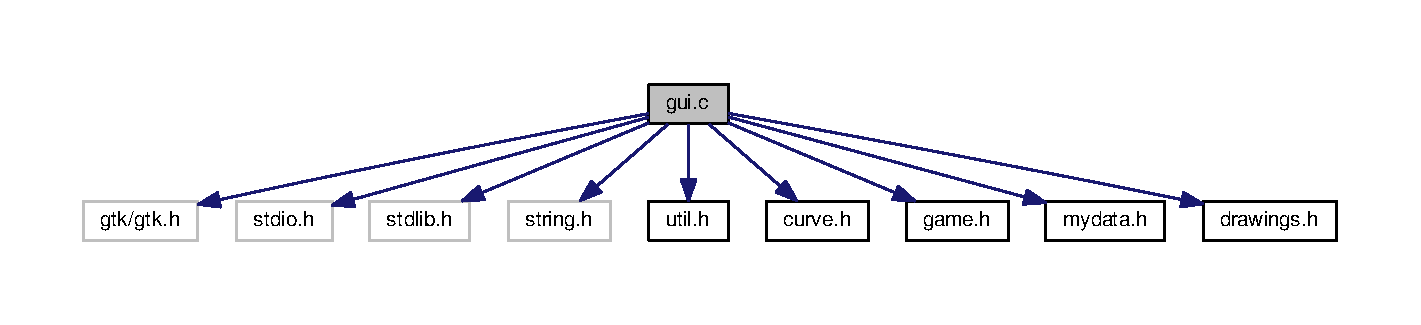
\includegraphics[width=350pt]{gui_8c__incl}
\end{center}
\end{figure}
\subsection*{Functions}
\begin{DoxyCompactItemize}
\item 
void {\bfseries on\+\_\+radio\+\_\+toggled} (Gtk\+Widget $\ast$widget, gpointer data)\hypertarget{gui_8c_a6ca222f09039aa6cade376bf8bcf2b1c}{}\label{gui_8c_a6ca222f09039aa6cade376bf8bcf2b1c}

\item 
void {\bfseries on\+\_\+bsp\+\_\+radio\+\_\+toggled} (Gtk\+Widget $\ast$widget, gpointer data)\hypertarget{gui_8c_a4123e3f2c87a4ae827b4f5b059d113f4}{}\label{gui_8c_a4123e3f2c87a4ae827b4f5b059d113f4}

\item 
void \hyperlink{gui_8c_a07fba752f7282a864c6903d2d6005630}{window\+\_\+init} (Gtk\+Application $\ast$app, gpointer user\+\_\+data)
\begin{DoxyCompactList}\small\item\em Fonction d\textquotesingle{}initialisation de la fenêtre. \end{DoxyCompactList}\item 
void \hyperlink{gui_8c_a9510208f9f6152cfd54fec0e3483e88b}{editing\+\_\+init} (\hyperlink{struct_mydata}{Mydata} $\ast$data)
\begin{DoxyCompactList}\small\item\em Fonction d\textquotesingle{}initialisation de la frame d\textquotesingle{}edition. \end{DoxyCompactList}\item 
void \hyperlink{gui_8c_a3f3ccd906ad3169a4a6b1c477aa0043f}{player\+Stats\+Frame\+\_\+init} (\hyperlink{struct_mydata}{Mydata} $\ast$data)
\begin{DoxyCompactList}\small\item\em Fonction d\textquotesingle{}initialisation de la frame des statistiques du joueur. \end{DoxyCompactList}\item 
void \hyperlink{gui_8c_a375a492ec90ae451c9877a2ef406bb5f}{layout\+\_\+init} (gpointer user\+\_\+data)
\begin{DoxyCompactList}\small\item\em Fonction d\textquotesingle{}initialisation du layout. \end{DoxyCompactList}\item 
void \hyperlink{gui_8c_a4e37c8e97d01196c66e6598294816853}{status\+\_\+init} (gpointer user\+\_\+data)
\begin{DoxyCompactList}\small\item\em Fonction d\textquotesingle{}initialisation de la barre de status. \end{DoxyCompactList}\end{DoxyCompactItemize}


\subsection{Detailed Description}
Interface graphique. 

\begin{DoxyAuthor}{Author}
Gaëtan Perrot 
\end{DoxyAuthor}
\begin{DoxyVersion}{Version}
0.\+1 
\end{DoxyVersion}
\begin{DoxyDate}{Date}
23 avril 2017
\end{DoxyDate}
Interface graphique 

\subsection{Function Documentation}
\index{gui.\+c@{gui.\+c}!editing\+\_\+init@{editing\+\_\+init}}
\index{editing\+\_\+init@{editing\+\_\+init}!gui.\+c@{gui.\+c}}
\subsubsection[{\texorpdfstring{editing\+\_\+init(\+Mydata $\ast$data)}{editing_init(Mydata *data)}}]{\setlength{\rightskip}{0pt plus 5cm}void editing\+\_\+init (
\begin{DoxyParamCaption}
\item[{{\bf Mydata} $\ast$}]{data}
\end{DoxyParamCaption}
)}\hypertarget{gui_8c_a9510208f9f6152cfd54fec0e3483e88b}{}\label{gui_8c_a9510208f9f6152cfd54fec0e3483e88b}


Fonction d\textquotesingle{}initialisation de la frame d\textquotesingle{}edition. 


\begin{DoxyParams}{Parameters}
{\em self} & Objet \hyperlink{struct_mydata}{Mydata} \\
\hline
\end{DoxyParams}
\begin{DoxyReturn}{Returns}
void 
\end{DoxyReturn}
\index{gui.\+c@{gui.\+c}!layout\+\_\+init@{layout\+\_\+init}}
\index{layout\+\_\+init@{layout\+\_\+init}!gui.\+c@{gui.\+c}}
\subsubsection[{\texorpdfstring{layout\+\_\+init(gpointer user\+\_\+data)}{layout_init(gpointer user_data)}}]{\setlength{\rightskip}{0pt plus 5cm}void layout\+\_\+init (
\begin{DoxyParamCaption}
\item[{gpointer}]{user\+\_\+data}
\end{DoxyParamCaption}
)}\hypertarget{gui_8c_a375a492ec90ae451c9877a2ef406bb5f}{}\label{gui_8c_a375a492ec90ae451c9877a2ef406bb5f}


Fonction d\textquotesingle{}initialisation du layout. 


\begin{DoxyParams}{Parameters}
{\em self} & gpointer Objet \hyperlink{struct_mydata}{Mydata} \\
\hline
\end{DoxyParams}
\begin{DoxyReturn}{Returns}
void 
\end{DoxyReturn}
\index{gui.\+c@{gui.\+c}!player\+Stats\+Frame\+\_\+init@{player\+Stats\+Frame\+\_\+init}}
\index{player\+Stats\+Frame\+\_\+init@{player\+Stats\+Frame\+\_\+init}!gui.\+c@{gui.\+c}}
\subsubsection[{\texorpdfstring{player\+Stats\+Frame\+\_\+init(\+Mydata $\ast$data)}{playerStatsFrame_init(Mydata *data)}}]{\setlength{\rightskip}{0pt plus 5cm}void player\+Stats\+Frame\+\_\+init (
\begin{DoxyParamCaption}
\item[{{\bf Mydata} $\ast$}]{data}
\end{DoxyParamCaption}
)}\hypertarget{gui_8c_a3f3ccd906ad3169a4a6b1c477aa0043f}{}\label{gui_8c_a3f3ccd906ad3169a4a6b1c477aa0043f}


Fonction d\textquotesingle{}initialisation de la frame des statistiques du joueur. 


\begin{DoxyParams}{Parameters}
{\em self} & Objet \hyperlink{struct_mydata}{Mydata} \\
\hline
\end{DoxyParams}
\begin{DoxyReturn}{Returns}
void 
\end{DoxyReturn}
\index{gui.\+c@{gui.\+c}!status\+\_\+init@{status\+\_\+init}}
\index{status\+\_\+init@{status\+\_\+init}!gui.\+c@{gui.\+c}}
\subsubsection[{\texorpdfstring{status\+\_\+init(gpointer user\+\_\+data)}{status_init(gpointer user_data)}}]{\setlength{\rightskip}{0pt plus 5cm}void status\+\_\+init (
\begin{DoxyParamCaption}
\item[{gpointer}]{user\+\_\+data}
\end{DoxyParamCaption}
)}\hypertarget{gui_8c_a4e37c8e97d01196c66e6598294816853}{}\label{gui_8c_a4e37c8e97d01196c66e6598294816853}


Fonction d\textquotesingle{}initialisation de la barre de status. 


\begin{DoxyParams}{Parameters}
{\em self} & gpointer Objet \hyperlink{struct_mydata}{Mydata} \\
\hline
\end{DoxyParams}
\begin{DoxyReturn}{Returns}
void 
\end{DoxyReturn}
\index{gui.\+c@{gui.\+c}!window\+\_\+init@{window\+\_\+init}}
\index{window\+\_\+init@{window\+\_\+init}!gui.\+c@{gui.\+c}}
\subsubsection[{\texorpdfstring{window\+\_\+init(\+Gtk\+Application $\ast$app, gpointer user\+\_\+data)}{window_init(GtkApplication *app, gpointer user_data)}}]{\setlength{\rightskip}{0pt plus 5cm}void window\+\_\+init (
\begin{DoxyParamCaption}
\item[{Gtk\+Application $\ast$}]{app, }
\item[{gpointer}]{user\+\_\+data}
\end{DoxyParamCaption}
)}\hypertarget{gui_8c_a07fba752f7282a864c6903d2d6005630}{}\label{gui_8c_a07fba752f7282a864c6903d2d6005630}


Fonction d\textquotesingle{}initialisation de la fenêtre. 


\begin{DoxyParams}{Parameters}
{\em self} & Gtk\+Application L\textquotesingle{}application, gpointer objet \hyperlink{struct_mydata}{Mydata} \\
\hline
\end{DoxyParams}
\begin{DoxyReturn}{Returns}
void 
\end{DoxyReturn}

\hypertarget{gui_8h}{}\section{gui.\+h File Reference}
\label{gui_8h}\index{gui.\+h@{gui.\+h}}


Interface graphique.  


This graph shows which files directly or indirectly include this file\+:
\nopagebreak
\begin{figure}[H]
\begin{center}
\leavevmode
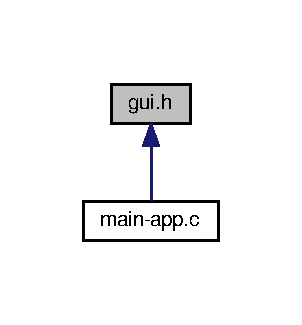
\includegraphics[width=145pt]{gui_8h__dep__incl}
\end{center}
\end{figure}
\subsection*{Functions}
\begin{DoxyCompactItemize}
\item 
void \hyperlink{gui_8h_a07fba752f7282a864c6903d2d6005630}{window\+\_\+init} (Gtk\+Application $\ast$app, gpointer user\+\_\+data)
\begin{DoxyCompactList}\small\item\em Fonction d\textquotesingle{}initialisation de la fenêtre. \end{DoxyCompactList}\item 
void \hyperlink{gui_8h_a9510208f9f6152cfd54fec0e3483e88b}{editing\+\_\+init} (\hyperlink{struct_mydata}{Mydata} $\ast$data)
\begin{DoxyCompactList}\small\item\em Fonction d\textquotesingle{}initialisation de la frame d\textquotesingle{}edition. \end{DoxyCompactList}\item 
void \hyperlink{gui_8h_a3f3ccd906ad3169a4a6b1c477aa0043f}{player\+Stats\+Frame\+\_\+init} (\hyperlink{struct_mydata}{Mydata} $\ast$data)
\begin{DoxyCompactList}\small\item\em Fonction d\textquotesingle{}initialisation de la frame des statistiques du joueur. \end{DoxyCompactList}\item 
void \hyperlink{gui_8h_a375a492ec90ae451c9877a2ef406bb5f}{layout\+\_\+init} (gpointer user\+\_\+data)
\begin{DoxyCompactList}\small\item\em Fonction d\textquotesingle{}initialisation du layout. \end{DoxyCompactList}\item 
void \hyperlink{gui_8h_a4e37c8e97d01196c66e6598294816853}{status\+\_\+init} (gpointer user\+\_\+data)
\begin{DoxyCompactList}\small\item\em Fonction d\textquotesingle{}initialisation de la barre de status. \end{DoxyCompactList}\end{DoxyCompactItemize}


\subsection{Detailed Description}
Interface graphique. 

\begin{DoxyAuthor}{Author}
Gaëtan Perrot 
\end{DoxyAuthor}
\begin{DoxyVersion}{Version}
0.\+1 
\end{DoxyVersion}
\begin{DoxyDate}{Date}
23 avril 2017
\end{DoxyDate}
Interface graphique 

\subsection{Function Documentation}
\index{gui.\+h@{gui.\+h}!editing\+\_\+init@{editing\+\_\+init}}
\index{editing\+\_\+init@{editing\+\_\+init}!gui.\+h@{gui.\+h}}
\subsubsection[{\texorpdfstring{editing\+\_\+init(\+Mydata $\ast$data)}{editing_init(Mydata *data)}}]{\setlength{\rightskip}{0pt plus 5cm}void editing\+\_\+init (
\begin{DoxyParamCaption}
\item[{{\bf Mydata} $\ast$}]{data}
\end{DoxyParamCaption}
)}\hypertarget{gui_8h_a9510208f9f6152cfd54fec0e3483e88b}{}\label{gui_8h_a9510208f9f6152cfd54fec0e3483e88b}


Fonction d\textquotesingle{}initialisation de la frame d\textquotesingle{}edition. 


\begin{DoxyParams}{Parameters}
{\em self} & Objet \hyperlink{struct_mydata}{Mydata} \\
\hline
\end{DoxyParams}
\begin{DoxyReturn}{Returns}
void 
\end{DoxyReturn}
\index{gui.\+h@{gui.\+h}!layout\+\_\+init@{layout\+\_\+init}}
\index{layout\+\_\+init@{layout\+\_\+init}!gui.\+h@{gui.\+h}}
\subsubsection[{\texorpdfstring{layout\+\_\+init(gpointer user\+\_\+data)}{layout_init(gpointer user_data)}}]{\setlength{\rightskip}{0pt plus 5cm}void layout\+\_\+init (
\begin{DoxyParamCaption}
\item[{gpointer}]{user\+\_\+data}
\end{DoxyParamCaption}
)}\hypertarget{gui_8h_a375a492ec90ae451c9877a2ef406bb5f}{}\label{gui_8h_a375a492ec90ae451c9877a2ef406bb5f}


Fonction d\textquotesingle{}initialisation du layout. 


\begin{DoxyParams}{Parameters}
{\em self} & gpointer Objet \hyperlink{struct_mydata}{Mydata} \\
\hline
\end{DoxyParams}
\begin{DoxyReturn}{Returns}
void 
\end{DoxyReturn}
\index{gui.\+h@{gui.\+h}!player\+Stats\+Frame\+\_\+init@{player\+Stats\+Frame\+\_\+init}}
\index{player\+Stats\+Frame\+\_\+init@{player\+Stats\+Frame\+\_\+init}!gui.\+h@{gui.\+h}}
\subsubsection[{\texorpdfstring{player\+Stats\+Frame\+\_\+init(\+Mydata $\ast$data)}{playerStatsFrame_init(Mydata *data)}}]{\setlength{\rightskip}{0pt plus 5cm}void player\+Stats\+Frame\+\_\+init (
\begin{DoxyParamCaption}
\item[{{\bf Mydata} $\ast$}]{data}
\end{DoxyParamCaption}
)}\hypertarget{gui_8h_a3f3ccd906ad3169a4a6b1c477aa0043f}{}\label{gui_8h_a3f3ccd906ad3169a4a6b1c477aa0043f}


Fonction d\textquotesingle{}initialisation de la frame des statistiques du joueur. 


\begin{DoxyParams}{Parameters}
{\em self} & Objet \hyperlink{struct_mydata}{Mydata} \\
\hline
\end{DoxyParams}
\begin{DoxyReturn}{Returns}
void 
\end{DoxyReturn}
\index{gui.\+h@{gui.\+h}!status\+\_\+init@{status\+\_\+init}}
\index{status\+\_\+init@{status\+\_\+init}!gui.\+h@{gui.\+h}}
\subsubsection[{\texorpdfstring{status\+\_\+init(gpointer user\+\_\+data)}{status_init(gpointer user_data)}}]{\setlength{\rightskip}{0pt plus 5cm}void status\+\_\+init (
\begin{DoxyParamCaption}
\item[{gpointer}]{user\+\_\+data}
\end{DoxyParamCaption}
)}\hypertarget{gui_8h_a4e37c8e97d01196c66e6598294816853}{}\label{gui_8h_a4e37c8e97d01196c66e6598294816853}


Fonction d\textquotesingle{}initialisation de la barre de status. 


\begin{DoxyParams}{Parameters}
{\em self} & gpointer Objet \hyperlink{struct_mydata}{Mydata} \\
\hline
\end{DoxyParams}
\begin{DoxyReturn}{Returns}
void 
\end{DoxyReturn}
\index{gui.\+h@{gui.\+h}!window\+\_\+init@{window\+\_\+init}}
\index{window\+\_\+init@{window\+\_\+init}!gui.\+h@{gui.\+h}}
\subsubsection[{\texorpdfstring{window\+\_\+init(\+Gtk\+Application $\ast$app, gpointer user\+\_\+data)}{window_init(GtkApplication *app, gpointer user_data)}}]{\setlength{\rightskip}{0pt plus 5cm}void window\+\_\+init (
\begin{DoxyParamCaption}
\item[{Gtk\+Application $\ast$}]{app, }
\item[{gpointer}]{user\+\_\+data}
\end{DoxyParamCaption}
)}\hypertarget{gui_8h_a07fba752f7282a864c6903d2d6005630}{}\label{gui_8h_a07fba752f7282a864c6903d2d6005630}


Fonction d\textquotesingle{}initialisation de la fenêtre. 


\begin{DoxyParams}{Parameters}
{\em self} & Gtk\+Application L\textquotesingle{}application, gpointer objet \hyperlink{struct_mydata}{Mydata} \\
\hline
\end{DoxyParams}
\begin{DoxyReturn}{Returns}
void 
\end{DoxyReturn}

\hypertarget{main-app_8c}{}\section{main-\/app.c File Reference}
\label{main-app_8c}\index{main-\/app.\+c@{main-\/app.\+c}}


Main App.  


{\ttfamily \#include $<$gtk/gtk.\+h$>$}\\*
{\ttfamily \#include $<$stdio.\+h$>$}\\*
{\ttfamily \#include $<$stdlib.\+h$>$}\\*
{\ttfamily \#include $<$locale.\+h$>$}\\*
{\ttfamily \#include \char`\"{}curve.\+h\char`\"{}}\\*
{\ttfamily \#include \char`\"{}util.\+h\char`\"{}}\\*
{\ttfamily \#include \char`\"{}game.\+h\char`\"{}}\\*
{\ttfamily \#include \char`\"{}mydata.\+h\char`\"{}}\\*
{\ttfamily \#include \char`\"{}drawings.\+h\char`\"{}}\\*
{\ttfamily \#include \char`\"{}menus.\+h\char`\"{}}\\*
{\ttfamily \#include \char`\"{}gui.\+h\char`\"{}}\\*
Include dependency graph for main-\/app.c\+:
\nopagebreak
\begin{figure}[H]
\begin{center}
\leavevmode
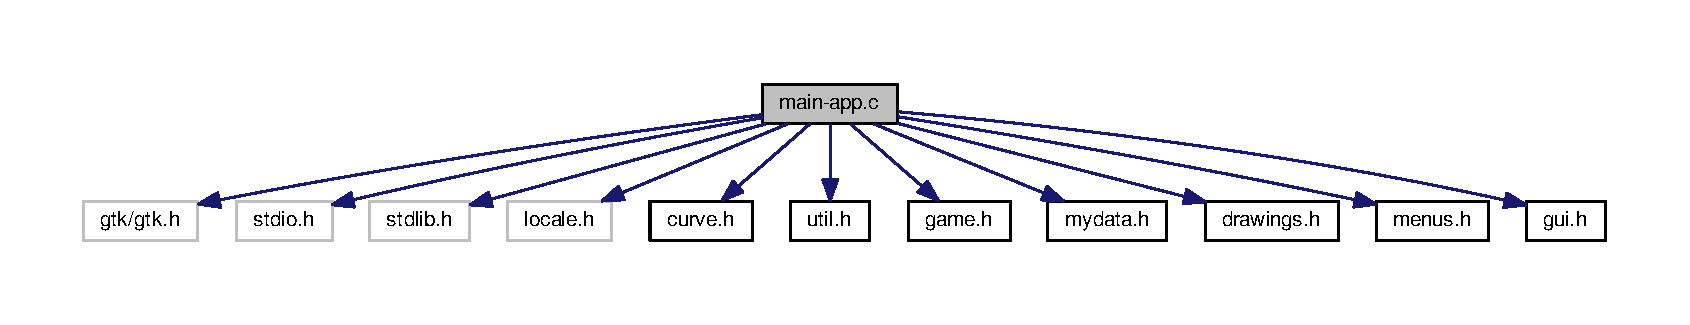
\includegraphics[width=350pt]{main-app_8c__incl}
\end{center}
\end{figure}
\subsection*{Functions}
\begin{DoxyCompactItemize}
\item 
void {\bfseries on\+\_\+app\+\_\+activate} (Gtk\+Application $\ast$app, gpointer user\+\_\+data)\hypertarget{main-app_8c_a7d38dcf9a1859bd3823a68d1e70c1b16}{}\label{main-app_8c_a7d38dcf9a1859bd3823a68d1e70c1b16}

\item 
int {\bfseries main} (int argc, char $\ast$argv\mbox{[}$\,$\mbox{]})\hypertarget{main-app_8c_a0ddf1224851353fc92bfbff6f499fa97}{}\label{main-app_8c_a0ddf1224851353fc92bfbff6f499fa97}

\end{DoxyCompactItemize}
\subsection*{Variables}
\begin{DoxyCompactItemize}
\item 
int {\bfseries timeout}\hypertarget{main-app_8c_a493b57f443cc38b3d3df9c1e584d9d82}{}\label{main-app_8c_a493b57f443cc38b3d3df9c1e584d9d82}

\end{DoxyCompactItemize}


\subsection{Detailed Description}
Main App. 

\begin{DoxyAuthor}{Author}
Gaëtan Perrot 
\end{DoxyAuthor}
\begin{DoxyVersion}{Version}
0.\+1 
\end{DoxyVersion}
\begin{DoxyDate}{Date}
23 avril 2017
\end{DoxyDate}
Main App, fonctions principale 
\hypertarget{menus_8c}{}\section{menus.\+c File Reference}
\label{menus_8c}\index{menus.\+c@{menus.\+c}}


Gestion des menus et évènements des menus.  


{\ttfamily \#include $<$gtk/gtk.\+h$>$}\\*
{\ttfamily \#include $<$stdio.\+h$>$}\\*
{\ttfamily \#include $<$stdlib.\+h$>$}\\*
{\ttfamily \#include $<$string.\+h$>$}\\*
{\ttfamily \#include \char`\"{}util.\+h\char`\"{}}\\*
{\ttfamily \#include \char`\"{}curve.\+h\char`\"{}}\\*
{\ttfamily \#include \char`\"{}game.\+h\char`\"{}}\\*
{\ttfamily \#include \char`\"{}mydata.\+h\char`\"{}}\\*
{\ttfamily \#include \char`\"{}drawings.\+h\char`\"{}}\\*
{\ttfamily \#include $<$errno.\+h$>$}\\*
{\ttfamily \#include \char`\"{}menus.\+h\char`\"{}}\\*
Include dependency graph for menus.\+c\+:
\nopagebreak
\begin{figure}[H]
\begin{center}
\leavevmode
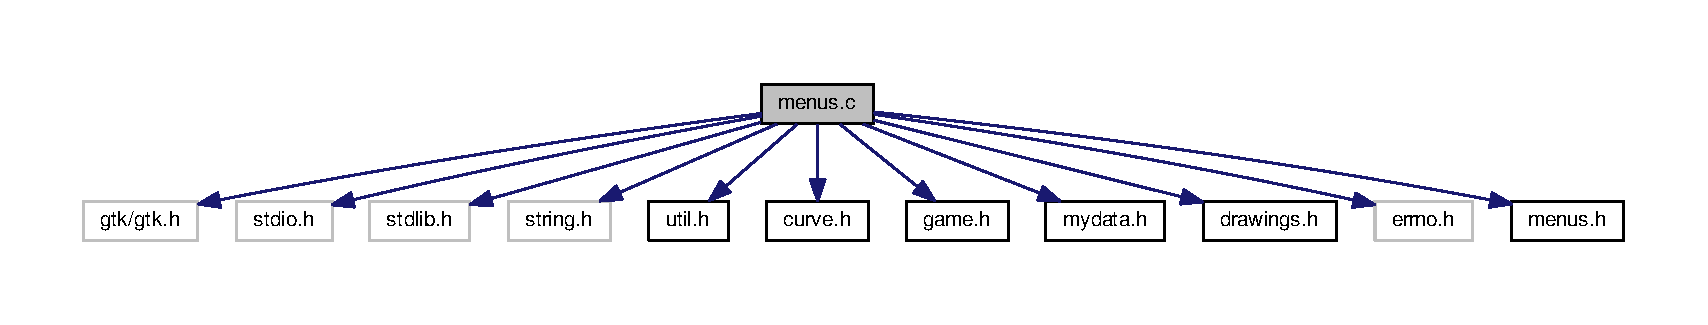
\includegraphics[width=350pt]{menus_8c__incl}
\end{center}
\end{figure}
\subsection*{Functions}
\begin{DoxyCompactItemize}
\item 
void {\bfseries on\+\_\+item\+\_\+about\+\_\+activate} (Gtk\+Widget $\ast$widget, gpointer data)\hypertarget{menus_8c_a483069984e9c28368a7cdb290dc492ec}{}\label{menus_8c_a483069984e9c28368a7cdb290dc492ec}

\item 
void {\bfseries on\+\_\+item\+\_\+new\+\_\+level\+\_\+activate} (Gtk\+Widget $\ast$widget, gpointer data)\hypertarget{menus_8c_a8bec92dd556d88acddcad577339eea84}{}\label{menus_8c_a8bec92dd556d88acddcad577339eea84}

\item 
void {\bfseries on\+\_\+item\+\_\+load\+\_\+level\+\_\+activate} (Gtk\+Widget $\ast$widget, gpointer data)\hypertarget{menus_8c_a292bbcd443bfeb2e679aec61a223eb97}{}\label{menus_8c_a292bbcd443bfeb2e679aec61a223eb97}

\item 
void {\bfseries on\+\_\+item\+\_\+save\+\_\+activate} (Gtk\+Widget $\ast$widget, gpointer data)\hypertarget{menus_8c_ac4407e9753540f83753db8306706da45}{}\label{menus_8c_ac4407e9753540f83753db8306706da45}

\item 
void {\bfseries on\+\_\+item\+\_\+new\+\_\+game\+\_\+activate} (Gtk\+Widget $\ast$widget, gpointer data)\hypertarget{menus_8c_afa2eed0906d57526de082ebfc47d0d5e}{}\label{menus_8c_afa2eed0906d57526de082ebfc47d0d5e}

\item 
void {\bfseries on\+\_\+item\+\_\+re\+\_\+start\+\_\+activate} (Gtk\+Widget $\ast$widget, gpointer data)\hypertarget{menus_8c_a3b3de28f66315eab8b11f5096afca7a9}{}\label{menus_8c_a3b3de28f66315eab8b11f5096afca7a9}

\item 
void {\bfseries on\+\_\+item\+\_\+start\+\_\+activate} (Gtk\+Widget $\ast$widget, gpointer data)\hypertarget{menus_8c_af550d46dd3f330884fed8040484c29a4}{}\label{menus_8c_af550d46dd3f330884fed8040484c29a4}

\item 
void {\bfseries on\+\_\+item\+\_\+pause\+\_\+activate} (Gtk\+Widget $\ast$widget, gpointer data)\hypertarget{menus_8c_a37be1c3b040f799a639a0c24d78db711}{}\label{menus_8c_a37be1c3b040f799a639a0c24d78db711}

\item 
void {\bfseries on\+\_\+item\+\_\+quit\+\_\+activate} (Gtk\+Widget $\ast$widget, gpointer data)\hypertarget{menus_8c_afaf10adeec6a216446d47dbcc906ae61}{}\label{menus_8c_afaf10adeec6a216446d47dbcc906ae61}

\item 
void {\bfseries on\+\_\+item\+\_\+edit\+\_\+activate} (Gtk\+Check\+Menu\+Item $\ast$widget, gpointer data)\hypertarget{menus_8c_a0d06139c3e585e70f00e008ea37b87da}{}\label{menus_8c_a0d06139c3e585e70f00e008ea37b87da}

\item 
void \hyperlink{menus_8c_aab0e8657d765a92956625a9c43a449f0}{menu\+\_\+init} (gpointer user\+\_\+data)
\begin{DoxyCompactList}\small\item\em Fonction d\textquotesingle{}initialisation du menu. \end{DoxyCompactList}\end{DoxyCompactItemize}


\subsection{Detailed Description}
Gestion des menus et évènements des menus. 

\begin{DoxyAuthor}{Author}
Gaëtan Perrot 
\end{DoxyAuthor}
\begin{DoxyVersion}{Version}
0.\+1 
\end{DoxyVersion}
\begin{DoxyDate}{Date}
23 avril 2017
\end{DoxyDate}
Gestion des menus et évènements des menus 

\subsection{Function Documentation}
\index{menus.\+c@{menus.\+c}!menu\+\_\+init@{menu\+\_\+init}}
\index{menu\+\_\+init@{menu\+\_\+init}!menus.\+c@{menus.\+c}}
\subsubsection[{\texorpdfstring{menu\+\_\+init(gpointer user\+\_\+data)}{menu_init(gpointer user_data)}}]{\setlength{\rightskip}{0pt plus 5cm}void menu\+\_\+init (
\begin{DoxyParamCaption}
\item[{gpointer}]{user\+\_\+data}
\end{DoxyParamCaption}
)}\hypertarget{menus_8c_aab0e8657d765a92956625a9c43a449f0}{}\label{menus_8c_aab0e8657d765a92956625a9c43a449f0}


Fonction d\textquotesingle{}initialisation du menu. 


\begin{DoxyParams}{Parameters}
{\em self} & Un objet gpointer (\hyperlink{struct_mydata}{Mydata}). \\
\hline
\end{DoxyParams}
\begin{DoxyReturn}{Returns}
void 
\end{DoxyReturn}

\hypertarget{menus_8h}{}\section{menus.\+h File Reference}
\label{menus_8h}\index{menus.\+h@{menus.\+h}}


Gestion des menus et évènements des menus.  


This graph shows which files directly or indirectly include this file\+:
\nopagebreak
\begin{figure}[H]
\begin{center}
\leavevmode
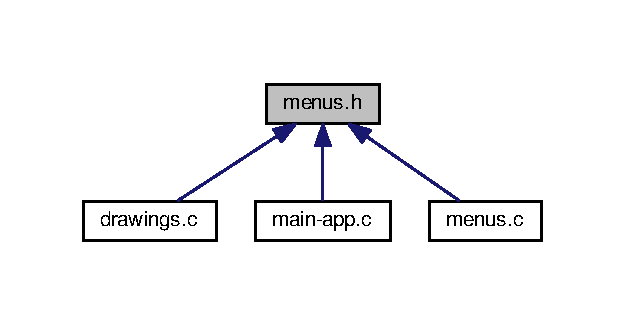
\includegraphics[width=300pt]{menus_8h__dep__incl}
\end{center}
\end{figure}
\subsection*{Functions}
\begin{DoxyCompactItemize}
\item 
void \hyperlink{menus_8h_aab0e8657d765a92956625a9c43a449f0}{menu\+\_\+init} (gpointer user\+\_\+data)
\begin{DoxyCompactList}\small\item\em Fonction d\textquotesingle{}initialisation du menu. \end{DoxyCompactList}\end{DoxyCompactItemize}


\subsection{Detailed Description}
Gestion des menus et évènements des menus. 

\begin{DoxyAuthor}{Author}
Gaëtan Perrot 
\end{DoxyAuthor}
\begin{DoxyVersion}{Version}
0.\+1 
\end{DoxyVersion}
\begin{DoxyDate}{Date}
23 avril 2017
\end{DoxyDate}
Gestion des menus et évènements des menus 

\subsection{Function Documentation}
\index{menus.\+h@{menus.\+h}!menu\+\_\+init@{menu\+\_\+init}}
\index{menu\+\_\+init@{menu\+\_\+init}!menus.\+h@{menus.\+h}}
\subsubsection[{\texorpdfstring{menu\+\_\+init(gpointer user\+\_\+data)}{menu_init(gpointer user_data)}}]{\setlength{\rightskip}{0pt plus 5cm}void menu\+\_\+init (
\begin{DoxyParamCaption}
\item[{gpointer}]{user\+\_\+data}
\end{DoxyParamCaption}
)}\hypertarget{menus_8h_aab0e8657d765a92956625a9c43a449f0}{}\label{menus_8h_aab0e8657d765a92956625a9c43a449f0}


Fonction d\textquotesingle{}initialisation du menu. 


\begin{DoxyParams}{Parameters}
{\em self} & Un objet gpointer (\hyperlink{struct_mydata}{Mydata}). \\
\hline
\end{DoxyParams}
\begin{DoxyReturn}{Returns}
void 
\end{DoxyReturn}

\hypertarget{mydata_8c}{}\section{mydata.\+c File Reference}
\label{mydata_8c}\index{mydata.\+c@{mydata.\+c}}


\hyperlink{struct_mydata}{Mydata} structure avec les objets principaux.  


{\ttfamily \#include $<$gtk/gtk.\+h$>$}\\*
{\ttfamily \#include $<$stdio.\+h$>$}\\*
{\ttfamily \#include $<$stdlib.\+h$>$}\\*
{\ttfamily \#include \char`\"{}curve.\+h\char`\"{}}\\*
{\ttfamily \#include \char`\"{}game.\+h\char`\"{}}\\*
{\ttfamily \#include \char`\"{}mydata.\+h\char`\"{}}\\*
Include dependency graph for mydata.\+c\+:
\nopagebreak
\begin{figure}[H]
\begin{center}
\leavevmode
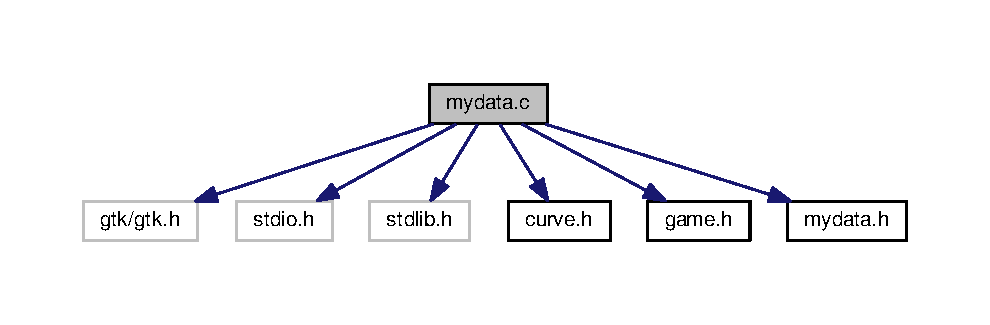
\includegraphics[width=350pt]{mydata_8c__incl}
\end{center}
\end{figure}
\subsection*{Macros}
\begin{DoxyCompactItemize}
\item 
\#define {\bfseries M\+Y\+D\+A\+T\+A\+\_\+\+M\+A\+G\+IC}~0x46\+E\+A7\+E05\hypertarget{mydata_8c_a41621b13791afbf5f5a88ec2c3fe5ac2}{}\label{mydata_8c_a41621b13791afbf5f5a88ec2c3fe5ac2}

\end{DoxyCompactItemize}
\subsection*{Functions}
\begin{DoxyCompactItemize}
\item 
\hyperlink{struct_mydata}{Mydata} $\ast$ \hyperlink{mydata_8c_a94e9cd97b633a6bc5845fb9e3f7b5a42}{get\+\_\+mydata} (gpointer data)
\begin{DoxyCompactList}\small\item\em Fonction de récupération de l\textquotesingle{}objet \hyperlink{struct_mydata}{Mydata} à partir d\textquotesingle{}un gpointeur. \end{DoxyCompactList}\item 
void \hyperlink{mydata_8c_a0b1e96cdd4d1a8b4f6cef990070887bf}{init\+\_\+mydata} (\hyperlink{struct_mydata}{Mydata} $\ast$my)
\begin{DoxyCompactList}\small\item\em Fonction d\textquotesingle{}initialisation de l\textquotesingle{}objet \hyperlink{struct_mydata}{Mydata}. \end{DoxyCompactList}\item 
void \hyperlink{mydata_8c_aa351d5e2597fba2a6af74589ab4553da}{set\+\_\+edit\+\_\+mode} (\hyperlink{struct_mydata}{Mydata} $\ast$data, int mode)
\begin{DoxyCompactList}\small\item\em Fonction de Gestion de l\textquotesingle{}édition \+: Curves / Controls. \end{DoxyCompactList}\end{DoxyCompactItemize}


\subsection{Detailed Description}
\hyperlink{struct_mydata}{Mydata} structure avec les objets principaux. 

\begin{DoxyAuthor}{Author}
Gaëtan Perrot 
\end{DoxyAuthor}
\begin{DoxyVersion}{Version}
0.\+1 
\end{DoxyVersion}
\begin{DoxyDate}{Date}
23 avril 2017
\end{DoxyDate}
\hyperlink{struct_mydata}{Mydata} structure avec les objets principaux 

\subsection{Function Documentation}
\index{mydata.\+c@{mydata.\+c}!get\+\_\+mydata@{get\+\_\+mydata}}
\index{get\+\_\+mydata@{get\+\_\+mydata}!mydata.\+c@{mydata.\+c}}
\subsubsection[{\texorpdfstring{get\+\_\+mydata(gpointer data)}{get_mydata(gpointer data)}}]{\setlength{\rightskip}{0pt plus 5cm}{\bf Mydata} $\ast$ get\+\_\+mydata (
\begin{DoxyParamCaption}
\item[{gpointer}]{data}
\end{DoxyParamCaption}
)}\hypertarget{mydata_8c_a94e9cd97b633a6bc5845fb9e3f7b5a42}{}\label{mydata_8c_a94e9cd97b633a6bc5845fb9e3f7b5a42}


Fonction de récupération de l\textquotesingle{}objet \hyperlink{struct_mydata}{Mydata} à partir d\textquotesingle{}un gpointeur. 


\begin{DoxyParams}{Parameters}
{\em self} & Un \hyperlink{struct_mydata}{Mydata} passé sous forme de gpointer \\
\hline
\end{DoxyParams}
\begin{DoxyReturn}{Returns}
\hyperlink{struct_mydata}{Mydata} $\ast$ si aucune erreur, N\+U\+LL sinon. 
\end{DoxyReturn}
\index{mydata.\+c@{mydata.\+c}!init\+\_\+mydata@{init\+\_\+mydata}}
\index{init\+\_\+mydata@{init\+\_\+mydata}!mydata.\+c@{mydata.\+c}}
\subsubsection[{\texorpdfstring{init\+\_\+mydata(\+Mydata $\ast$my)}{init_mydata(Mydata *my)}}]{\setlength{\rightskip}{0pt plus 5cm}void init\+\_\+mydata (
\begin{DoxyParamCaption}
\item[{{\bf Mydata} $\ast$}]{my}
\end{DoxyParamCaption}
)}\hypertarget{mydata_8c_a0b1e96cdd4d1a8b4f6cef990070887bf}{}\label{mydata_8c_a0b1e96cdd4d1a8b4f6cef990070887bf}


Fonction d\textquotesingle{}initialisation de l\textquotesingle{}objet \hyperlink{struct_mydata}{Mydata}. 


\begin{DoxyParams}{Parameters}
{\em self} & Un objet \hyperlink{struct_mydata}{Mydata} \\
\hline
\end{DoxyParams}
\begin{DoxyReturn}{Returns}
void 
\end{DoxyReturn}
\index{mydata.\+c@{mydata.\+c}!set\+\_\+edit\+\_\+mode@{set\+\_\+edit\+\_\+mode}}
\index{set\+\_\+edit\+\_\+mode@{set\+\_\+edit\+\_\+mode}!mydata.\+c@{mydata.\+c}}
\subsubsection[{\texorpdfstring{set\+\_\+edit\+\_\+mode(\+Mydata $\ast$data, int mode)}{set_edit_mode(Mydata *data, int mode)}}]{\setlength{\rightskip}{0pt plus 5cm}void set\+\_\+edit\+\_\+mode (
\begin{DoxyParamCaption}
\item[{{\bf Mydata} $\ast$}]{data, }
\item[{int}]{mode}
\end{DoxyParamCaption}
)}\hypertarget{mydata_8c_aa351d5e2597fba2a6af74589ab4553da}{}\label{mydata_8c_aa351d5e2597fba2a6af74589ab4553da}


Fonction de Gestion de l\textquotesingle{}édition \+: Curves / Controls. 


\begin{DoxyParams}{Parameters}
{\em self} & Un objet \hyperlink{struct_mydata}{Mydata} ainsi que le mode d\textquotesingle{}edition, un entier. \\
\hline
\end{DoxyParams}
\begin{DoxyReturn}{Returns}
void 
\end{DoxyReturn}

\hypertarget{mydata_8h}{}\section{mydata.\+h File Reference}
\label{mydata_8h}\index{mydata.\+h@{mydata.\+h}}


\hyperlink{struct_mydata}{Mydata} structure avec les objets principaux.  


This graph shows which files directly or indirectly include this file\+:
\nopagebreak
\begin{figure}[H]
\begin{center}
\leavevmode
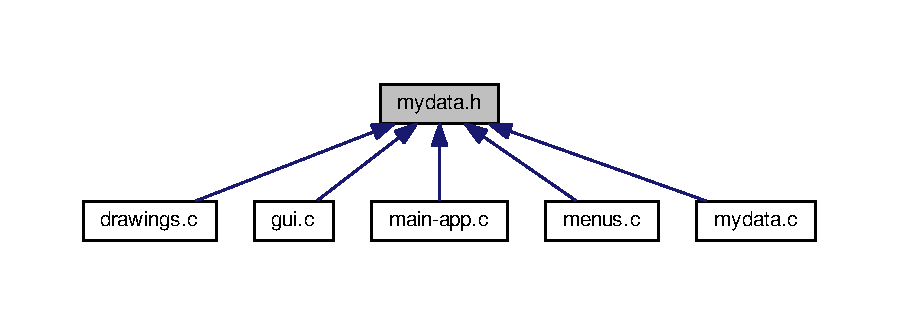
\includegraphics[width=350pt]{mydata_8h__dep__incl}
\end{center}
\end{figure}
\subsection*{Data Structures}
\begin{DoxyCompactItemize}
\item 
struct \hyperlink{struct_mydata}{Mydata}
\begin{DoxyCompactList}\small\item\em Objet contenant les informations pour un \hyperlink{struct_mydata}{Mydata}. \end{DoxyCompactList}\end{DoxyCompactItemize}
\subsection*{Enumerations}
\begin{DoxyCompactItemize}
\item 
enum \hyperlink{mydata_8h_a1a2ae634179b86b212d6e6d79f1cdf27}{const\+\_\+edit} \{ \\*
{\bfseries E\+D\+I\+T\+\_\+\+N\+O\+NE}, 
{\bfseries E\+D\+I\+T\+\_\+\+A\+D\+D\+\_\+\+C\+U\+R\+VE}, 
{\bfseries E\+D\+I\+T\+\_\+\+M\+O\+V\+E\+\_\+\+C\+U\+R\+VE}, 
{\bfseries E\+D\+I\+T\+\_\+\+R\+E\+M\+O\+V\+E\+\_\+\+C\+U\+R\+VE}, 
\\*
{\bfseries E\+D\+I\+T\+\_\+\+A\+D\+D\+\_\+\+C\+O\+N\+T\+R\+OL}, 
{\bfseries E\+D\+I\+T\+\_\+\+M\+O\+V\+E\+\_\+\+C\+O\+N\+T\+R\+OL}, 
{\bfseries E\+D\+I\+T\+\_\+\+R\+E\+M\+O\+V\+E\+\_\+\+C\+O\+N\+T\+R\+OL}, 
{\bfseries E\+D\+I\+T\+\_\+\+L\+A\+ST}
 \}\begin{DoxyCompactList}\small\item\em Constantes du choix du mode d\textquotesingle{}edition. \end{DoxyCompactList}
\item 
enum \hyperlink{mydata_8h_ab4fdc64ac4f04b45213b265f134b9ffa}{const\+\_\+mode} \{ {\bfseries B\+S\+P\+\_\+\+F\+I\+R\+ST}, 
{\bfseries B\+S\+P\+\_\+\+P\+R\+O\+L\+O\+NG}, 
{\bfseries B\+S\+P\+\_\+\+L\+A\+ST}
 \}\begin{DoxyCompactList}\small\item\em Constantes du choix du mode de création des courbes. \end{DoxyCompactList}
\end{DoxyCompactItemize}
\subsection*{Functions}
\begin{DoxyCompactItemize}
\item 
\hyperlink{struct_mydata}{Mydata} $\ast$ \hyperlink{mydata_8h_ad38e3f1616cb48aa2f13c5796cd9ab96}{get\+\_\+mydata} (gpointer data)
\begin{DoxyCompactList}\small\item\em Fonction de récupération de l\textquotesingle{}objet \hyperlink{struct_mydata}{Mydata} à partir d\textquotesingle{}un gpointeur. \end{DoxyCompactList}\item 
void \hyperlink{mydata_8h_a0b1e96cdd4d1a8b4f6cef990070887bf}{init\+\_\+mydata} (\hyperlink{struct_mydata}{Mydata} $\ast$my)
\begin{DoxyCompactList}\small\item\em Fonction d\textquotesingle{}initialisation de l\textquotesingle{}objet \hyperlink{struct_mydata}{Mydata}. \end{DoxyCompactList}\item 
void \hyperlink{mydata_8h_aa351d5e2597fba2a6af74589ab4553da}{set\+\_\+edit\+\_\+mode} (\hyperlink{struct_mydata}{Mydata} $\ast$data, int mode)
\begin{DoxyCompactList}\small\item\em Fonction de Gestion de l\textquotesingle{}édition \+: Curves / Controls. \end{DoxyCompactList}\end{DoxyCompactItemize}


\subsection{Detailed Description}
\hyperlink{struct_mydata}{Mydata} structure avec les objets principaux. 

\begin{DoxyAuthor}{Author}
Gaëtan Perrot 
\end{DoxyAuthor}
\begin{DoxyVersion}{Version}
0.\+1 
\end{DoxyVersion}
\begin{DoxyDate}{Date}
23 avril 2017
\end{DoxyDate}
\hyperlink{struct_mydata}{Mydata} structure avec les objets principaux 

\subsection{Enumeration Type Documentation}
\index{mydata.\+h@{mydata.\+h}!const\+\_\+edit@{const\+\_\+edit}}
\index{const\+\_\+edit@{const\+\_\+edit}!mydata.\+h@{mydata.\+h}}
\subsubsection[{\texorpdfstring{const\+\_\+edit}{const_edit}}]{\setlength{\rightskip}{0pt plus 5cm}enum {\bf const\+\_\+edit}}\hypertarget{mydata_8h_a1a2ae634179b86b212d6e6d79f1cdf27}{}\label{mydata_8h_a1a2ae634179b86b212d6e6d79f1cdf27}


Constantes du choix du mode d\textquotesingle{}edition. 

const\+\_\+edit est une série de constantes prédéfinie pour les choix du mode d\textquotesingle{}edition \index{mydata.\+h@{mydata.\+h}!const\+\_\+mode@{const\+\_\+mode}}
\index{const\+\_\+mode@{const\+\_\+mode}!mydata.\+h@{mydata.\+h}}
\subsubsection[{\texorpdfstring{const\+\_\+mode}{const_mode}}]{\setlength{\rightskip}{0pt plus 5cm}enum {\bf const\+\_\+mode}}\hypertarget{mydata_8h_ab4fdc64ac4f04b45213b265f134b9ffa}{}\label{mydata_8h_ab4fdc64ac4f04b45213b265f134b9ffa}


Constantes du choix du mode de création des courbes. 

const\+\_\+mode est une série de constantes prédéfinie pour les choix du mode de création des courbes 

\subsection{Function Documentation}
\index{mydata.\+h@{mydata.\+h}!get\+\_\+mydata@{get\+\_\+mydata}}
\index{get\+\_\+mydata@{get\+\_\+mydata}!mydata.\+h@{mydata.\+h}}
\subsubsection[{\texorpdfstring{get\+\_\+mydata(gpointer data)}{get_mydata(gpointer data)}}]{\setlength{\rightskip}{0pt plus 5cm}{\bf Mydata}$\ast$ get\+\_\+mydata (
\begin{DoxyParamCaption}
\item[{gpointer}]{data}
\end{DoxyParamCaption}
)}\hypertarget{mydata_8h_ad38e3f1616cb48aa2f13c5796cd9ab96}{}\label{mydata_8h_ad38e3f1616cb48aa2f13c5796cd9ab96}


Fonction de récupération de l\textquotesingle{}objet \hyperlink{struct_mydata}{Mydata} à partir d\textquotesingle{}un gpointeur. 


\begin{DoxyParams}{Parameters}
{\em self} & Un \hyperlink{struct_mydata}{Mydata} passé sous forme de gpointer \\
\hline
\end{DoxyParams}
\begin{DoxyReturn}{Returns}
\hyperlink{struct_mydata}{Mydata} $\ast$ si aucune erreur, N\+U\+LL sinon. 
\end{DoxyReturn}
\index{mydata.\+h@{mydata.\+h}!init\+\_\+mydata@{init\+\_\+mydata}}
\index{init\+\_\+mydata@{init\+\_\+mydata}!mydata.\+h@{mydata.\+h}}
\subsubsection[{\texorpdfstring{init\+\_\+mydata(\+Mydata $\ast$my)}{init_mydata(Mydata *my)}}]{\setlength{\rightskip}{0pt plus 5cm}void init\+\_\+mydata (
\begin{DoxyParamCaption}
\item[{{\bf Mydata} $\ast$}]{my}
\end{DoxyParamCaption}
)}\hypertarget{mydata_8h_a0b1e96cdd4d1a8b4f6cef990070887bf}{}\label{mydata_8h_a0b1e96cdd4d1a8b4f6cef990070887bf}


Fonction d\textquotesingle{}initialisation de l\textquotesingle{}objet \hyperlink{struct_mydata}{Mydata}. 


\begin{DoxyParams}{Parameters}
{\em self} & Un objet \hyperlink{struct_mydata}{Mydata} \\
\hline
\end{DoxyParams}
\begin{DoxyReturn}{Returns}
void 
\end{DoxyReturn}
\index{mydata.\+h@{mydata.\+h}!set\+\_\+edit\+\_\+mode@{set\+\_\+edit\+\_\+mode}}
\index{set\+\_\+edit\+\_\+mode@{set\+\_\+edit\+\_\+mode}!mydata.\+h@{mydata.\+h}}
\subsubsection[{\texorpdfstring{set\+\_\+edit\+\_\+mode(\+Mydata $\ast$data, int mode)}{set_edit_mode(Mydata *data, int mode)}}]{\setlength{\rightskip}{0pt plus 5cm}void set\+\_\+edit\+\_\+mode (
\begin{DoxyParamCaption}
\item[{{\bf Mydata} $\ast$}]{data, }
\item[{int}]{mode}
\end{DoxyParamCaption}
)}\hypertarget{mydata_8h_aa351d5e2597fba2a6af74589ab4553da}{}\label{mydata_8h_aa351d5e2597fba2a6af74589ab4553da}


Fonction de Gestion de l\textquotesingle{}édition \+: Curves / Controls. 


\begin{DoxyParams}{Parameters}
{\em self} & Un objet \hyperlink{struct_mydata}{Mydata} ainsi que le mode d\textquotesingle{}edition, un entier. \\
\hline
\end{DoxyParams}
\begin{DoxyReturn}{Returns}
void 
\end{DoxyReturn}

\hypertarget{util_8c}{}\section{util.\+c File Reference}
\label{util_8c}\index{util.\+c@{util.\+c}}


Fonctions utiles.  


{\ttfamily \#include $<$gtk/gtk.\+h$>$}\\*
{\ttfamily \#include $<$stdio.\+h$>$}\\*
{\ttfamily \#include \char`\"{}util.\+h\char`\"{}}\\*
Include dependency graph for util.\+c\+:
\nopagebreak
\begin{figure}[H]
\begin{center}
\leavevmode
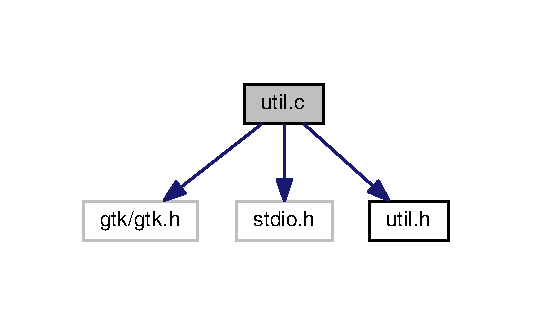
\includegraphics[width=256pt]{util_8c__incl}
\end{center}
\end{figure}
\subsection*{Functions}
\begin{DoxyCompactItemize}
\item 
void \hyperlink{util_8c_a4692be361eab8d079776e945613ea9e8}{refresh\+\_\+area} (Gtk\+Widget $\ast$area)
\begin{DoxyCompactList}\small\item\em Fonction de rafraichissement de l\textquotesingle{}area. \end{DoxyCompactList}\item 
void \hyperlink{util_8c_a1a411315b6a84a92684787962bee7bef}{set\+\_\+status} (Gtk\+Widget $\ast$status, const char $\ast$format,...)
\begin{DoxyCompactList}\small\item\em Fonction pour mettre à jour la barre de status Mise à jour de la barre de statut. \end{DoxyCompactList}\item 
int \hyperlink{util_8c_af008852dadb1e4471a8589eabfeebecb}{recup\+Time} ()
\begin{DoxyCompactList}\small\item\em Fonction de récupération du l\textquotesingle{}heure en seconde. \end{DoxyCompactList}\end{DoxyCompactItemize}


\subsection{Detailed Description}
Fonctions utiles. 

\begin{DoxyAuthor}{Author}
Gaëtan Perrot 
\end{DoxyAuthor}
\begin{DoxyVersion}{Version}
0.\+1 
\end{DoxyVersion}
\begin{DoxyDate}{Date}
23 avril 2017
\end{DoxyDate}
Fonctions utiles 

\subsection{Function Documentation}
\index{util.\+c@{util.\+c}!recup\+Time@{recup\+Time}}
\index{recup\+Time@{recup\+Time}!util.\+c@{util.\+c}}
\subsubsection[{\texorpdfstring{recup\+Time()}{recupTime()}}]{\setlength{\rightskip}{0pt plus 5cm}int recup\+Time (
\begin{DoxyParamCaption}
{}
\end{DoxyParamCaption}
)}\hypertarget{util_8c_af008852dadb1e4471a8589eabfeebecb}{}\label{util_8c_af008852dadb1e4471a8589eabfeebecb}


Fonction de récupération du l\textquotesingle{}heure en seconde. 


\begin{DoxyParams}{Parameters}
{\em self} & \\
\hline
\end{DoxyParams}
\begin{DoxyReturn}{Returns}
int l\textquotesingle{}heure actuelle en seconde 
\end{DoxyReturn}
\index{util.\+c@{util.\+c}!refresh\+\_\+area@{refresh\+\_\+area}}
\index{refresh\+\_\+area@{refresh\+\_\+area}!util.\+c@{util.\+c}}
\subsubsection[{\texorpdfstring{refresh\+\_\+area(\+Gtk\+Widget $\ast$area)}{refresh_area(GtkWidget *area)}}]{\setlength{\rightskip}{0pt plus 5cm}void refresh\+\_\+area (
\begin{DoxyParamCaption}
\item[{Gtk\+Widget $\ast$}]{area}
\end{DoxyParamCaption}
)}\hypertarget{util_8c_a4692be361eab8d079776e945613ea9e8}{}\label{util_8c_a4692be361eab8d079776e945613ea9e8}


Fonction de rafraichissement de l\textquotesingle{}area. 


\begin{DoxyParams}{Parameters}
{\em self} & Un objet Gtk\+Widget notre area \\
\hline
\end{DoxyParams}
\begin{DoxyReturn}{Returns}
void 
\end{DoxyReturn}
\index{util.\+c@{util.\+c}!set\+\_\+status@{set\+\_\+status}}
\index{set\+\_\+status@{set\+\_\+status}!util.\+c@{util.\+c}}
\subsubsection[{\texorpdfstring{set\+\_\+status(\+Gtk\+Widget $\ast$status, const char $\ast$format,...)}{set_status(GtkWidget *status, const char *format,...)}}]{\setlength{\rightskip}{0pt plus 5cm}void set\+\_\+status (
\begin{DoxyParamCaption}
\item[{Gtk\+Widget $\ast$}]{status, }
\item[{const char $\ast$}]{format, }
\item[{}]{...}
\end{DoxyParamCaption}
)}\hypertarget{util_8c_a1a411315b6a84a92684787962bee7bef}{}\label{util_8c_a1a411315b6a84a92684787962bee7bef}


Fonction pour mettre à jour la barre de status Mise à jour de la barre de statut. 

Fonction pour mettre à jour la barre de status.


\begin{DoxyParams}{Parameters}
{\em self} & Un objet Gtk\+Widget notre barre de status, une chaine, et des paramètres optionnels pour construire la chaine \\
\hline
\end{DoxyParams}
\begin{DoxyReturn}{Returns}
void 
\end{DoxyReturn}

\hypertarget{util_8h}{}\section{util.\+h File Reference}
\label{util_8h}\index{util.\+h@{util.\+h}}


Fonctions utiles.  


This graph shows which files directly or indirectly include this file\+:
\nopagebreak
\begin{figure}[H]
\begin{center}
\leavevmode
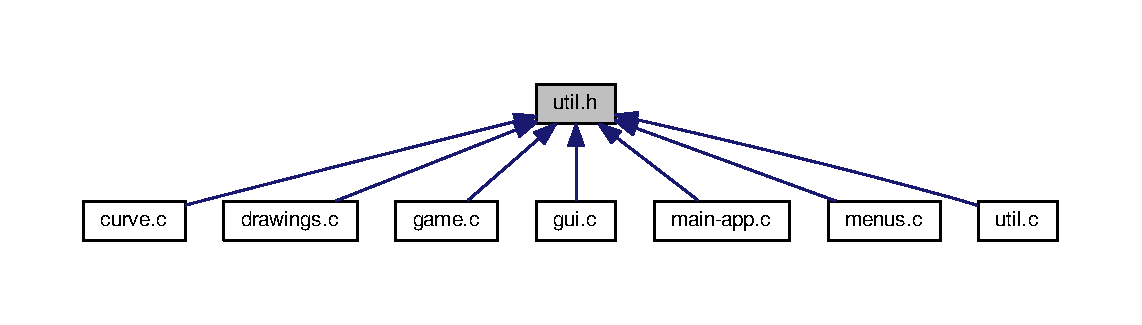
\includegraphics[width=350pt]{util_8h__dep__incl}
\end{center}
\end{figure}
\subsection*{Macros}
\begin{DoxyCompactItemize}
\item 
\#define {\bfseries S\+A\+V\+E\+\_\+\+F\+I\+L\+E\+\_\+\+D\+E\+F\+A\+U\+LT}~\char`\"{}Untitled.\+track\char`\"{}\hypertarget{util_8h_a5acb4d53cc0b3b7cd11c95eab0a97f09}{}\label{util_8h_a5acb4d53cc0b3b7cd11c95eab0a97f09}

\end{DoxyCompactItemize}
\subsection*{Functions}
\begin{DoxyCompactItemize}
\item 
void \hyperlink{util_8h_a4692be361eab8d079776e945613ea9e8}{refresh\+\_\+area} (Gtk\+Widget $\ast$area)
\begin{DoxyCompactList}\small\item\em Fonction de rafraichissement de l\textquotesingle{}area. \end{DoxyCompactList}\item 
void \hyperlink{util_8h_a1a411315b6a84a92684787962bee7bef}{set\+\_\+status} (Gtk\+Widget $\ast$status, const char $\ast$format,...)
\begin{DoxyCompactList}\small\item\em Fonction pour mettre à jour la barre de status Mise à jour de la barre de statut. \end{DoxyCompactList}\item 
int \hyperlink{util_8h_af008852dadb1e4471a8589eabfeebecb}{recup\+Time} ()
\begin{DoxyCompactList}\small\item\em Fonction de récupération du l\textquotesingle{}heure en seconde. \end{DoxyCompactList}\end{DoxyCompactItemize}


\subsection{Detailed Description}
Fonctions utiles. 

\begin{DoxyAuthor}{Author}
Gaëtan Perrot 
\end{DoxyAuthor}
\begin{DoxyVersion}{Version}
0.\+1 
\end{DoxyVersion}
\begin{DoxyDate}{Date}
23 avril 2017
\end{DoxyDate}
Fonctions utiles 

\subsection{Function Documentation}
\index{util.\+h@{util.\+h}!recup\+Time@{recup\+Time}}
\index{recup\+Time@{recup\+Time}!util.\+h@{util.\+h}}
\subsubsection[{\texorpdfstring{recup\+Time()}{recupTime()}}]{\setlength{\rightskip}{0pt plus 5cm}int recup\+Time (
\begin{DoxyParamCaption}
{}
\end{DoxyParamCaption}
)}\hypertarget{util_8h_af008852dadb1e4471a8589eabfeebecb}{}\label{util_8h_af008852dadb1e4471a8589eabfeebecb}


Fonction de récupération du l\textquotesingle{}heure en seconde. 


\begin{DoxyParams}{Parameters}
{\em self} & \\
\hline
\end{DoxyParams}
\begin{DoxyReturn}{Returns}
int l\textquotesingle{}heure actuelle en seconde 
\end{DoxyReturn}
\index{util.\+h@{util.\+h}!refresh\+\_\+area@{refresh\+\_\+area}}
\index{refresh\+\_\+area@{refresh\+\_\+area}!util.\+h@{util.\+h}}
\subsubsection[{\texorpdfstring{refresh\+\_\+area(\+Gtk\+Widget $\ast$area)}{refresh_area(GtkWidget *area)}}]{\setlength{\rightskip}{0pt plus 5cm}void refresh\+\_\+area (
\begin{DoxyParamCaption}
\item[{Gtk\+Widget $\ast$}]{area}
\end{DoxyParamCaption}
)}\hypertarget{util_8h_a4692be361eab8d079776e945613ea9e8}{}\label{util_8h_a4692be361eab8d079776e945613ea9e8}


Fonction de rafraichissement de l\textquotesingle{}area. 


\begin{DoxyParams}{Parameters}
{\em self} & Un objet Gtk\+Widget notre area \\
\hline
\end{DoxyParams}
\begin{DoxyReturn}{Returns}
void 
\end{DoxyReturn}
\index{util.\+h@{util.\+h}!set\+\_\+status@{set\+\_\+status}}
\index{set\+\_\+status@{set\+\_\+status}!util.\+h@{util.\+h}}
\subsubsection[{\texorpdfstring{set\+\_\+status(\+Gtk\+Widget $\ast$status, const char $\ast$format,...)}{set_status(GtkWidget *status, const char *format,...)}}]{\setlength{\rightskip}{0pt plus 5cm}void set\+\_\+status (
\begin{DoxyParamCaption}
\item[{Gtk\+Widget $\ast$}]{status, }
\item[{const char $\ast$}]{format, }
\item[{}]{...}
\end{DoxyParamCaption}
)}\hypertarget{util_8h_a1a411315b6a84a92684787962bee7bef}{}\label{util_8h_a1a411315b6a84a92684787962bee7bef}


Fonction pour mettre à jour la barre de status Mise à jour de la barre de statut. 

Fonction pour mettre à jour la barre de status.


\begin{DoxyParams}{Parameters}
{\em self} & Un objet Gtk\+Widget notre barre de status, une chaine, et des paramètres optionnels pour construire la chaine \\
\hline
\end{DoxyParams}
\begin{DoxyReturn}{Returns}
void 
\end{DoxyReturn}

%--- End generated contents ---

% Index
\backmatter
\newpage
\phantomsection
\clearemptydoublepage
\addcontentsline{toc}{chapter}{Index}
\printindex

\end{document}
